%==============================================================================
%  BAO CAO DO AN / PROJECT REPORT
%  De tai: Dao ham & Khoi tao trong Deep Learning -- Backpropagation va
%          Parameter Initialization
%
%  BIEN DICH BANG XeLaTeX:
%      xelatex main  ->  bibtex main  ->  xelatex main  ->  xelatex main
%  (Overleaf: chon Menu > Compiler > XeLaTeX)
%==============================================================================
\documentclass[12pt,a4paper]{article}

% ---------- FONT & TIENG VIET (XeLaTeX) ----------
\usepackage{fontspec}
\setmainfont{Latin Modern Roman}
\usepackage[vietnamese]{babel}

% ---------- BO CUC & TIEN ICH ----------
\usepackage[a4paper,top=2.3cm,bottom=2.3cm,left=2.5cm,right=2.5cm]{geometry}
\usepackage{amsmath,amssymb,mathtools}
\usepackage{graphicx}
\usepackage{booktabs}
\usepackage{array}
\usepackage{float}
\usepackage{xcolor}
\usepackage{enumitem}
\usepackage{caption}
\usepackage{microtype}
\usepackage{tikz}
\usetikzlibrary{arrows.meta,positioning,calc,shapes.geometric}
\usepackage[unicode=true,hidelinks]{hyperref}
\usepackage[numbers,square,sort&compress]{natbib}
\bibliographystyle{IEEEtranN}
\usepackage{listings}

\setlist{itemsep=1.5pt,topsep=3pt,parsep=0pt}
\captionsetup{font=small,labelfont=bf}
\setlength{\parskip}{0.3em}
\renewcommand{\arraystretch}{1.15}
\setcounter{tocdepth}{2}
\bibsep=2pt

\definecolor{fcol}{RGB}{40,90,180}   % forward
\definecolor{bcol}{RGB}{190,60,50}   % backward
\definecolor{boxln}{RGB}{120,140,175}
\definecolor{codebg}{RGB}{245,245,248}
\definecolor{codekw}{RGB}{30,90,150}
\definecolor{codestr}{RGB}{140,90,40}
\definecolor{codecmt}{RGB}{110,120,110}

\lstset{
  basicstyle=\ttfamily\small,
  backgroundcolor=\color{codebg},
  keywordstyle=\color{codekw}\bfseries,
  stringstyle=\color{codestr},
  commentstyle=\color{codecmt}\itshape,
  breaklines=true,
  frame=single,
  rulecolor=\color{black!20},
  framesep=4pt,
  xleftmargin=4pt, xrightmargin=4pt,
  showstringspaces=false,
  columns=flexible,
  language=Python,
}

% Hop ``truc giac'': neu cach hieu don gian truoc khi vao ky thuat
\newenvironment{tructiep}[1][Cách hiểu đơn giản]
  {\par\smallskip\noindent\begin{tabular}{@{}p{0.35em}@{\hspace{6pt}}p{\dimexpr\linewidth-1.9em\relax}@{}}
   \textcolor{boxln}{\rule{2pt}{\baselineskip}} & \textbf{#1.}\enspace\ignorespaces}
  {\end{tabular}\par\smallskip}

\newcommand{\en}[1]{\textit{#1}}
\newcommand{\T}{^{\mathsf{T}}}

\hypersetup{pdftitle={Bao cao: Backpropagation va Parameter Initialization},
            pdfauthor={Nhom sinh vien}}

\addto\captionsvietnamese{\renewcommand{\refname}{Tài liệu tham khảo}}
\addto\captionsvietnamese{\renewcommand{\contentsname}{Mục lục}}
\addto\captionsvietnamese{\renewcommand{\listfigurename}{Danh mục hình}}
\addto\captionsvietnamese{\renewcommand{\listtablename}{Danh mục bảng}}
\addto\captionsvietnamese{\renewcommand{\appendixname}{Phụ lục}}

\begin{document}

%==============================================================================
% TRANG BIA
%==============================================================================
\begin{titlepage}
\centering
\vspace*{1.2cm}
{\large TRƯỜNG ĐẠI HỌC --- KHOA CÔNG NGHỆ THÔNG TIN}\\[0.3cm]
{\large Học phần: Trí tuệ nhân tạo / Deep Learning}\\[2.2cm]

{\Large\bfseries ĐẠO HÀM \& KHỞI TẠO TRONG DEEP LEARNING:}\\[0.4cm]
{\Large\bfseries BACKPROPAGATION VÀ PARAMETER INITIALIZATION}\\[0.6cm]
{\itshape Derivatives \& Initialization in Deep Learning: Backpropagation
and Parameter Initialization}\\[2.0cm]

\begin{tabular}{rl}
Tác giả: & Bùi Đức Quân \\
Đơn vị đào tạo: & Khoa Công nghệ Thông tin, Trường Đại học Công nghiệp Hà Nội \\
Nhóm thực hiện: & Nhóm sinh viên Deep Learning \\
Giảng viên hướng dẫn: & Bộ môn Trí tuệ nhân tạo \\
\end{tabular}

\vspace{1.2cm}
{\small Mã nguồn \& dữ liệu tái lập (reproducibility):\\
\url{https://github.com/quanbui/deep-learning-derivatives-init}\\
Commit tham chiếu gần nhất tại thời điểm biên soạn: \texttt{637eec4}
(xem lịch sử repo để tra đúng commit khớp bản PDF này)}

\vfill
{\large Tháng 9, 2026}
\end{titlepage}

\tableofcontents
\newpage
\listoffigures
\listoftables
\newpage

%==============================================================================
% 1. GIOI THIEU
%==============================================================================
\section{Giới thiệu}

Huấn luyện một mạng nơ-ron về bản chất là giải một bài toán tối ưu: tìm bộ
tham số $\theta$ (các ma trận trọng số $W$ và vector bias $b$) sao cho hàm
mất mát $L(\theta)$ nhỏ nhất có thể. Để giải bài toán này bằng Gradient
Descent, có hai câu hỏi bắt buộc phải trả lời trước khi nói đến việc ``huấn
luyện'':

\begin{enumerate}
\item \textbf{Tính gradient thế nào?} Một mạng thực tế có thể có hàng triệu
  tham số; tính $\partial L/\partial\theta_i$ cho từng tham số một cách
  ngây thơ (ví dụ bằng finite-difference) là không khả thi. Đây là vấn đề
  mà \textbf{Backpropagation} giải quyết.
\item \textbf{Bắt đầu từ đâu?} Gradient Descent chỉ di chuyển tham số theo
  hướng giảm loss \emph{cục bộ}, xuất phát từ giá trị khởi tạo $\theta_0$.
  Chọn $\theta_0$ sai có thể khiến mạng không bao giờ học được gì, bất kể
  thuật toán tối ưu tốt đến đâu. Đây là vấn đề của
  \textbf{Parameter Initialization}.
\end{enumerate}

Báo cáo này đi từ nền tảng toán học (đạo hàm, chain rule, computational
graph) tới hai chủ đề trên, xen kẽ trực giác trước rồi mới tới công thức và
ví dụ số, tránh trình bày Backpropagation như một ``thuật toán thần kỳ''
tách rời khỏi Giải tích. Phần thực nghiệm (Mục~\ref{sec:methodology}--\ref{sec:results})
kiểm chứng lại các kết luận lý thuyết bằng số liệu thật trên Fashion-MNIST,
không dùng số liệu minh hoạ giả định.

\begin{tructiep}[Sơ đồ tư duy của cả báo cáo]
Chain Rule $\to$ Computational Graph $\to$ đạo hàm cục bộ từng bước $\to$
Backpropagation (thuật toán \emph{tính} gradient hiệu quả) $\to$ Gradient
Descent/Optimizer (\emph{dùng} gradient đó để cập nhật tham số) --- và song
song: Initialization quyết định gradient có ``chảy'' được qua mạng sâu hay
không (Mục~\ref{sec:vanishing}), nên hai chủ đề của báo cáo thực chất là
hai mặt của cùng một câu hỏi: \emph{làm sao tín hiệu học (gradient) đi
xuyên suốt một mạng nhiều lớp mà không biến mất hay bùng nổ?}
\end{tructiep}

\subsection*{Bối cảnh: vì sao hai chủ đề này lại tách biệt thành hai bước
phát triển lịch sử}
\addcontentsline{toc}{subsection}{Bối cảnh lịch sử}

Hai chủ đề của báo cáo không xuất hiện cùng lúc trong lịch sử Deep
Learning --- Backpropagation được giải quyết trước, Initialization được
nhận ra là vấn đề riêng biệt \emph{sau}, khi các mạng ngày càng sâu hơn:

\begin{itemize}
\item \textbf{1986}: \citet{rumelhart1986learning} phổ biến rộng rãi
  Backpropagation như một phương pháp thực tế để huấn luyện mạng nhiều
  lớp (\en{multilayer perceptron}), dựa trên Chain Rule --- giải quyết
  \emph{câu hỏi 1} (tính gradient hiệu quả).
\item \textbf{Cuối thập niên 1990}: khi các mạng bắt đầu sâu hơn,
  \citet{lecun1998efficient} tổng hợp nhiều kinh nghiệm thực hành
  (\en{Efficient BackProp}), trong đó có khuyến nghị khởi tạo trọng số
  theo $1/\sqrt{n_{\text{in}}}$ --- mầm mống sớm của \emph{câu hỏi 2}
  (chọn điểm xuất phát), nhưng chưa có phân tích variance đầy đủ.
\item \textbf{2010}: \citet{glorot2010understanding} đưa ra phân tích
  variance có hệ thống đầu tiên (Xavier/Glorot initialization, cân bằng
  cả forward lẫn backward), giải thích rõ \emph{tại sao} initialization
  sai làm mạng sâu khó huấn luyện --- đúng bằng phân tích
  Mục~\ref{sec:vanishing} của báo cáo này.
\item \textbf{2015}: khi ReLU trở thành activation phổ biến nhất (thay
  Sigmoid/Tanh), \citet{he2015delving} nhận ra công thức Xavier không tối
  ưu cho ReLU (do ReLU không đối xứng quanh $0$) và đề xuất hiệu chỉnh
  ---He/Kaiming initialization --- cho phép huấn luyện các mạng sâu hơn
  đáng kể so với trước đó.
\end{itemize}

Ba mươi năm phát triển này chính là lý do báo cáo trình bày Initialization
như một chủ đề \emph{riêng}, không gộp chung vào Backpropagation dù cả
hai đều xoay quanh cùng một câu hỏi cốt lõi về gradient.

%==============================================================================
% 2. NEN TANG TOAN HOC
%==============================================================================
\section{Nền tảng toán học}

Các khái niệm trong mục này là kiến thức Giải tích/Đại số tuyến tính chuẩn,
trình bày lại theo hướng ứng dụng cho Deep Learning (tham khảo cách trình
bày tổng quát trong~\citet{bishop2006pattern} và~\citet{goodfellow2016deep}).

\subsection{Đạo hàm (Derivative)}

\begin{tructiep}
Đạo hàm trả lời câu hỏi: \emph{nếu nhích $x$ một chút, $y=f(x)$ đổi bao
nhiêu?} --- nó đo \textbf{độ nhạy} của đầu ra theo đầu vào tại một điểm.
\end{tructiep}

$$\frac{dy}{dx} = \lim_{h\to 0}\frac{f(x+h)-f(x)}{h}.$$

Ví dụ $y=x^2$: $dy/dx=2x$. Tại $x=1.5$, đạo hàm $=3$, nghĩa là quanh
$x=1.5$, nhích $x$ thêm một lượng nhỏ $h$ thì $y$ đổi xấp xỉ $3h$ (Hình~\ref{fig:deriv}
minh hoạ bằng tiếp tuyến).

\begin{figure}[H]
\centering
\begin{tikzpicture}[scale=1.0, >=Stealth]
\draw[->] (-2.6,0) -- (2.6,0) node[right] {$x$};
\draw[->] (0,-0.8) -- (0,5.6) node[above] {$y$};
\draw[fcol, thick, smooth, domain=-2.35:2.35, samples=60]
  plot (\x,{\x*\x}) node[right,black] {$y=x^2$};
\draw[bcol, thick, dashed, domain=0.6:2.4, samples=2]
  plot (\x,{2.25+3*(\x-1.5)}) node[right,black,font=\footnotesize]
  {tiếp tuyến tại $x=1.5$ (độ dốc $=3$)};
\filldraw[bcol] (1.5,2.25) circle (1.6pt);
\node[below] at (1.5,-0.05) {\footnotesize $x=1.5$};
\end{tikzpicture}
\caption{Đạo hàm $=$ độ dốc của tiếp tuyến $=$ độ nhạy cục bộ của $y$ theo $x$.}
\label{fig:deriv}
\end{figure}

\textbf{Vai trò trong Deep Learning.} ``$x$'' ở đây chính là một tham số
($w$ hay $b$) và ``$y$'' là hàm mất mát $L$. Đạo hàm $\partial L/\partial w$
cho biết: \emph{nếu tăng $w$ một chút, loss tăng hay giảm, nhanh cỡ nào?}
--- đây chính là ``tín hiệu học'' mà Gradient Descent dùng để sửa tham số.
Không có đạo hàm, mạng không biết nên chỉnh $w$ theo hướng nào.

\subsection{Đạo hàm riêng (Partial Derivative)}

Khi $L$ phụ thuộc nhiều biến cùng lúc ($L(w_1,w_2,\ldots,w_n)$ --- một
mạng thực tế có thể có hàng triệu $w_i$), đạo hàm riêng
$\partial L/\partial w_i$ giữ \emph{mọi biến khác cố định}, chỉ đo độ nhạy
của $L$ theo riêng $w_i$. Về công thức, tính giống hệt đạo hàm thường, chỉ
khác ở chỗ ta ``đóng băng'' các biến còn lại khi lấy vi phân.

\subsection{Gradient}

\begin{tructiep}
Gradient gộp toàn bộ đạo hàm riêng thành một vector --- giống như gộp ``độ
dốc theo từng hướng riêng lẻ'' thành một mũi tên chỉ hướng dốc nhất.
\end{tructiep}

$$\nabla_\theta L = \left(\frac{\partial L}{\partial\theta_1},\ \frac{\partial L}{\partial\theta_2},\ \ldots,\ \frac{\partial L}{\partial\theta_n}\right).$$

$\nabla_\theta L$ là hướng làm $L$ \emph{tăng} nhanh nhất tại điểm hiện tại
$\theta$; do đó $-\nabla_\theta L$ là hướng làm $L$ \emph{giảm} nhanh nhất
cục bộ --- đây là nền tảng của Gradient Descent (Mục~\ref{sec:bp_vs_gd}).
Lưu ý: gradient tự nó chỉ là một \emph{phép đo} (một vector), chưa phải là
một thuật toán cập nhật tham số.

\textbf{Vì sao chính xác là hướng dốc nhất?} Với một hướng đơn vị bất kỳ
$v$ ($\lVert v\rVert=1$), \textbf{đạo hàm theo hướng} (\en{directional
derivative}) đo tốc độ đổi của $L$ khi di chuyển theo $v$:
$$D_v L = \nabla_\theta L \cdot v = \lVert\nabla_\theta L\rVert\,\lVert v\rVert\cos\varphi = \lVert\nabla_\theta L\rVert\cos\varphi$$
($\varphi$ = góc giữa $\nabla_\theta L$ và $v$). Biểu thức này lớn nhất
khi $\cos\varphi=1$, tức $v$ \emph{cùng hướng} với $\nabla_\theta L$
($\varphi=0$) --- chứng minh trực tiếp gradient là hướng tăng nhanh nhất;
tương tự, $D_vL$ nhỏ nhất (âm nhiều nhất) khi $v$ \emph{ngược hướng}
gradient ($\varphi=180°$), tức hướng giảm nhanh nhất là $-\nabla_\theta L$.

\textbf{Ví dụ số} ($L(\theta_1,\theta_2)=\theta_1^2+2\theta_2^2$ tại
$\theta=(1,1)$): $\nabla L = (2\theta_1,\,4\theta_2) = (2,4)$,
$\lVert\nabla L\rVert=\sqrt{20}\approx4.47$. So sánh $D_vL$ theo 3 hướng
đơn vị khác nhau:
\begin{itemize}
\item $v=\nabla L/\lVert\nabla L\rVert\approx(0.447;\,0.894)$ (cùng hướng gradient): $D_vL=\sqrt{20}\approx4.47$ (lớn nhất).
\item $v=(1,0)$ (chỉ đổi $\theta_1$): $D_vL = (2,4)\cdot(1,0)=2$.
\item $v=-\nabla L/\lVert\nabla L\rVert\approx(-0.447;\,-0.894)$ (ngược hướng gradient): $D_vL=-\sqrt{20}\approx-4.47$ (nhỏ nhất --- giảm nhanh nhất).
\end{itemize}
Đúng như dự đoán: đi theo $-\nabla L$ cho tốc độ giảm $L$ nhanh hơn hẳn đi
theo $(1,0)$ hay bất kỳ hướng nào khác --- đây chính xác là lý do
Gradient Descent (Mục~\ref{sec:bp_vs_gd}) chọn hướng cập nhật
$-\nabla_\theta L$ chứ không phải hướng nào khác.

\subsection{Jacobian --- khi đầu ra không chỉ là một số}
\label{sec:jacobian}

Gradient $\nabla_\theta L$ ở trên chỉ áp dụng khi đầu ra là \emph{một số}
(loss $L$ luôn là một số). Nhưng bên trong mạng, nhiều phép biến đổi có
đầu ra là \emph{cả một vector} --- ví dụ $z=Wx+b$ với $x\in\mathbb R^n$,
$z\in\mathbb R^m$. Khi đó ``đạo hàm'' tổng quát thành một \textbf{ma trận
Jacobian}: mỗi hàng là gradient của một toạ độ đầu ra theo toàn bộ đầu vào.
$$J = \frac{\partial z}{\partial x} = \begin{pmatrix}
\dfrac{\partial z_1}{\partial x_1} & \cdots & \dfrac{\partial z_1}{\partial x_n} \\[4pt]
\vdots & \ddots & \vdots \\[2pt]
\dfrac{\partial z_m}{\partial x_1} & \cdots & \dfrac{\partial z_m}{\partial x_n}
\end{pmatrix} \in \mathbb R^{m\times n}.$$

\begin{tructiep}
Gradient là ``1 số $\to$ nhiều số'' (một hàng của Jacobian). Jacobian là
``nhiều số $\to$ nhiều số'' (toàn bộ ma trận). Backpropagation lan truyền
\emph{ngược} một vector "độ nhạy tích luỹ" qua từng Jacobian, không bao giờ
lập ra Jacobian đầy đủ (rất tốn bộ nhớ với mạng lớn) --- công thức hình
thức ở dưới gọi đúng tên phép toán này: \textbf{Vector--Jacobian Product}.
\end{tructiep}

\textbf{Vector--Jacobian Product (VJP) và Reverse-mode AD.} Xét một phép
biến đổi $v_{i+1}=f_i(v_i)$ với Jacobian cục bộ $J_i=\partial v_{i+1}/\partial v_i$.
Định nghĩa \textbf{cotangent} (hay \emph{adjoint}) tại nút $i$ là
$\bar v_i \triangleq \partial L/\partial v_i$ (cùng shape với $v_i$, luôn
xuất phát từ đạo hàm của \emph{một số vô hướng} $L$ --- đúng trường hợp
$L$ là hàm mất mát). Quy tắc chuỗi cho cotangent là:
$$\bar v_i = \bar v_{i+1}\,J_i \qquad \Big(\text{viết theo vector cột: } \bar v_i\T = J_i\T\,\bar v_{i+1}\T\Big).$$
Đây gọi là \textbf{Vector--Jacobian Product (VJP)}: nhân một \emph{vector}
($\bar v_{i+1}$) với Jacobian $J_i$, đi \emph{ngược} chiều forward --- khác
với \en{Jacobian--Vector Product (JVP)} của \textbf{forward-mode AD} (nhân
Jacobian với một vector tangent $\dot v_i$, đi \emph{xuôi} chiều forward:
$\dot v_{i+1}=J_i\dot v_i$). Bảng~\ref{tab:vjp_jvp} tóm tắt khác biệt.

\begin{table}[H]
\centering
\small
\begin{tabular}{@{}p{2.6cm}p{5.5cm}p{6.1cm}@{}}
\toprule
 & \textbf{Forward-mode (JVP)} & \textbf{Reverse-mode (VJP) --- Backprop} \\
\midrule
Lan truyền & Tangent $\dot v$ đi \emph{xuôi} theo forward pass & Cotangent $\bar v$ đi \emph{ngược} sau khi forward pass hoàn tất \\
Công thức & $\dot v_{i+1} = J_i\dot v_i$ & $\bar v_i = \bar v_{i+1}J_i$ \\
Chi phí cho $n_{\text{in}}\to1$ đầu ra & $O(n_{\text{in}})$ lượt (1 lượt/hướng vào) & $O(1)$ lượt --- đúng $1$ lượt cho \emph{mọi} tham số cùng lúc \\
Phù hợp khi & \#outputs $\gg$ \#inputs & \#inputs $\gg$ \#outputs (đúng trường hợp mạng nơ-ron: hàng triệu $\theta$, $1$ số $L$) \\
\bottomrule
\end{tabular}
\caption{Forward-mode (JVP) vs.\ Reverse-mode (VJP) automatic differentiation}
\label{tab:vjp_jvp}
\end{table}

Vì mạng nơ-ron luôn có \emph{rất nhiều} tham số nhưng chỉ \emph{một} loss
vô hướng, reverse-mode (VJP) luôn được chọn --- đây là lý do toán học
chính xác cho lập luận "hiệu quả hơn theo bậc độ lớn" đã nêu ở
Mục~\ref{sec:complexity}, không chỉ là quan sát thực nghiệm.

\textbf{Khớp chính xác với \texttt{torch.autograd}.} PyTorch ghi lại một
đồ thị tính toán (DAG) trong lúc forward: mỗi tensor kết quả giữ một con
trỏ \texttt{grad\_fn} trỏ tới một đối tượng \texttt{Function} biết cách
tính VJP của chính phép toán đó. Lời gọi \texttt{loss.backward()} duyệt
DAG này theo thứ tự tô-pô \emph{ngược}, và tại mỗi nút gọi đúng phương
thức
$$\texttt{grad\_input = Function.backward(ctx, grad\_output)}$$
--- ở đây \texttt{grad\_output} chính là $\bar v_{i+1}$ (cotangent nhận từ
phía sau) và \texttt{grad\_input} chính là $\bar v_i=\bar v_{i+1}J_i$ (VJP
vừa định nghĩa). Nói cách khác, \textbf{mỗi hàm \texttt{backward()} trong
PyTorch chính là lời giải tường minh của công thức VJP cho đúng một phép
toán}; toàn bộ autograd engine chỉ là cơ chế ghép nối các lời giải cục bộ
đó theo đúng thứ tự Chain Rule --- không có "phép màu" nào khác.

\textbf{Ví dụ}: với $z=Wx+b$ ($W\in\mathbb R^{m\times n}$), Jacobian của
$z$ theo $x$ chính là $W$: $\partial z/\partial x = W$, và VJP tương ứng
$\bar x=\bar zW$ không bao giờ cần dựng $W$ tường minh dưới dạng Jacobian
--- $W$ \emph{đã sẵn là} ma trận cần nhân. Với hàm kích hoạt $a=f(z)$ áp
dụng \emph{độc lập theo từng toạ độ} (mọi activation trong
Mục~\ref{sec:schemes} đều vậy), Jacobian của nó là một \textbf{ma trận
đường chéo} $\mathrm{diag}(f'(z_1),\ldots,f'(z_m))$, nên VJP
$\bar z=\bar a\,\mathrm{diag}(f'(z))$ rút gọn thành phép nhân từng phần tử
$\bar z=\bar a\odot f'(z)$ --- đây chính là lý do $\odot$ xuất hiện xuyên
suốt Mục~\ref{sec:scalar}--\ref{sec:matrixform}, thay vì một phép nhân ma
trận đầy đủ tốn $O(m^2)$ bộ nhớ mỗi lớp.

\subsection{Quy tắc chuỗi (Chain Rule)}
\label{sec:chainrule}

$$y = f(g(x)) \quad\Longrightarrow\quad \frac{dy}{dx} = \frac{dy}{dg}\cdot\frac{dg}{dx}.$$

\begin{tructiep}
$g$ biến đổi $x$ thành một đại lượng trung gian; $f$ biến đổi đại lượng đó
thành $y$. Độ nhạy tổng của $y$ theo $x$ = độ nhạy của $y$ theo đại lượng
trung gian, nhân với độ nhạy của đại lượng trung gian theo $x$ --- ``truyền
độ nhạy'' qua từng bước trung gian, giống truyền tin đồn qua một chuỗi
người: mức độ ``sai lệch'' tới người cuối phụ thuộc vào mức khuếch đại/suy
giảm ở \emph{mỗi} khâu trung gian.
\end{tructiep}

Một neuron đơn là một chuỗi biến đổi lồng nhau:
$$x \;\xrightarrow{\;z=wx+b\;}\; z \;\xrightarrow{\;a=\sigma(z)\;}\; a \;\xrightarrow{\;L=\mathrm{loss}(a,y)\;}\; L.$$
Áp dụng Chain Rule liên tiếp cho từng tham số:
$$\frac{\partial L}{\partial w} = \frac{\partial L}{\partial a}\cdot\frac{\partial a}{\partial z}\cdot\frac{\partial z}{\partial w}, \qquad
\frac{\partial L}{\partial b} = \frac{\partial L}{\partial a}\cdot\frac{\partial a}{\partial z}\cdot\frac{\partial z}{\partial b}, \qquad
\frac{\partial L}{\partial x} = \frac{\partial L}{\partial a}\cdot\frac{\partial a}{\partial z}\cdot\frac{\partial z}{\partial x}.$$
$\partial L/\partial w$ và $\partial L/\partial b$ dùng để \textbf{cập nhật
tham số của chính lớp này}; $\partial L/\partial x$ dùng để \textbf{tiếp
tục lan truyền ngược sang lớp phía trước} (vì $x$ chính là đầu ra của lớp
trước đó) --- đây là hạt giống của thuật toán Backpropagation ở
Mục~\ref{sec:backprop}.

\subsection{Đồ thị tính toán (Computational Graph)}
\label{sec:compgraph}

Một biểu thức toán phức tạp có thể vẽ thành một đồ thị có hướng: mỗi nút là
một phép toán cơ bản (cộng, nhân, hàm kích hoạt\ldots), mỗi cạnh mang một
giá trị trung gian. \textbf{Forward pass} đi từ trái sang phải, tính từng
giá trị; \textbf{backward pass} đi ngược lại, và tại \emph{mỗi} nút chỉ cần
biết đạo hàm cục bộ của riêng phép toán đó, rồi nhân dồn theo Chain Rule.
Đây là lý do Backpropagation không cần suy ra một công thức đóng
(closed-form) cho toàn mạng --- chỉ cần mỗi phép toán ``biết'' đạo hàm của
chính nó, và một cơ chế nhân dồn có hệ thống.

\begin{figure}[H]
\centering
\begin{tikzpicture}[
  node distance=15mm,
  op/.style={draw,circle,minimum size=9mm,font=\small},
  val/.style={font=\small},
  >=Stealth]
\node[val] (x) {$x$};
\node[op, right=of x] (z) {$z$};
\node[op, right=of z] (a) {$a$};
\node[op, right=of a] (L) {$L$};
\node[val, above=6mm of z] (w) {$w$};
\node[val, above=6mm of x, xshift=8mm] (b) {$b$};
\node[val, right=12mm of L] (y) {$y$};
\draw[->,fcol,thick] (x) -- node[below,font=\scriptsize]{$z=wx+b$} (z);
\draw[->,fcol,thick] (z) -- node[below,font=\scriptsize]{$a=\mathrm{ReLU}(z)$} (a);
\draw[->,fcol,thick] (a) -- node[below,font=\scriptsize]{$L=\tfrac12(a-y)^2$} (L);
\draw[->,fcol,thick] (w) -- (z);
\draw[->,fcol,thick] (b) to[bend right=15] (z);
\draw[->,fcol,thick] (y) -- (L);
\draw[->,bcol,thick,dashed] ($(z)+(0,-9mm)$) -- node[below,font=\scriptsize,bcol]{$\partial L/\partial z$} ($(x)+(0,-9mm)$);
\draw[->,bcol,thick,dashed] ($(a)+(0,-9mm)$) -- node[below,font=\scriptsize,bcol]{$\partial L/\partial a$} ($(z)+(0,-9mm)$);
\draw[->,bcol,thick,dashed] ($(L)+(0,-9mm)$) -- node[below,font=\scriptsize,bcol]{$\partial L/\partial L=1$} ($(a)+(0,-9mm)$);
\end{tikzpicture}
\caption{Computational graph của $z=wx+b \to a=\mathrm{ReLU}(z) \to L=\tfrac12(a-y)^2$.
Mũi tên xanh (liền) = forward; mũi tên đỏ (đứt) = backward, đi ngược đúng
theo các cạnh forward.}
\label{fig:compgraph}
\end{figure}

Đạo hàm cục bộ của từng nút trong Hình~\ref{fig:compgraph}:
$$\frac{\partial L}{\partial a}=a-y,\qquad
\frac{\partial a}{\partial z}=\mathrm{ReLU}'(z)=\begin{cases}1,& z>0\\0,& z< 0\end{cases},\qquad
\frac{\partial z}{\partial w}=x,\quad \frac{\partial z}{\partial b}=1,\quad \frac{\partial z}{\partial x}=w.$$

\textbf{Tại $z=0$: dưới đạo hàm (subgradient).} $\mathrm{ReLU}(z)=\max(0,z)$
\emph{không khả vi} tại $z=0$ (đồ thị có một "góc gãy", hai phía có độ dốc
khác nhau: $0$ bên trái, $1$ bên phải) --- đạo hàm thường không tồn tại tại
điểm này. Vì ReLU là hàm \textbf{lồi} (\en{convex}), công cụ thay thế đúng
đắn về giải tích là \textbf{tập dưới vi phân} (\en{subdifferential}):
$$\partial f(z_0) \triangleq \{\,c\in\mathbb R : f(z) \ge f(z_0) + c\,(z-z_0)\ \ \forall z\,\}$$
(tập mọi độ dốc $c$ sao cho đường thẳng qua $(z_0,f(z_0))$ độ dốc $c$ luôn
nằm \emph{dưới hoặc chạm} đồ thị $f$ --- với hàm khả vi thông thường, tập
này chỉ có đúng $1$ phần tử $=f'(z_0)$). Với $\mathrm{ReLU}$ tại $z_0=0$,
kiểm tra trực tiếp định nghĩa cho:
$$\partial\,\mathrm{ReLU}(0) = [0,1]$$
(mọi $c\in[0,1]$ đều thoả bất đẳng thức trên; xem chứng minh nhanh:
với $z\ge0$ cần $z\ge cz\Leftrightarrow c\le1$; với $z<0$ cần $0\ge cz
\Leftrightarrow c\ge0$). Về mặt lý thuyết, \textbf{bất kỳ} giá trị nào
trong $[0,1]$ đều là một dưới đạo hàm hợp lệ tại $z=0$.

\textbf{Quy ước kỹ thuật của framework.} Để có một con số \emph{duy nhất}
dùng trong backward pass (Mục~\ref{sec:matrixform} cần $f'(z)$ là một hàm
số, không phải một tập), PyTorch và hầu hết framework chọn cố định
$$\left.\frac{\partial\,\mathrm{ReLU}}{\partial z}\right\vert_{z=0} = 0$$
--- một lựa chọn \emph{hợp lệ} (nằm trong $[0,1]$) nhưng \emph{không duy
nhất về mặt toán học}. Lựa chọn này không gây vấn đề thực tế vì hai lý do:
(1) với $z$ liên tục (số thực dấu phẩy động), sự kiện $z$ \emph{đúng bằng}
$0$ tuyệt đối có xác suất gần như $0$ (tập đo-không) --- ngoại lệ đáng chú
ý duy nhất trong báo cáo này là chính kịch bản Zero-init
(Mục~\ref{sec:zero}), nơi $z\equiv0$ \emph{cho mọi} neuron một cách có chủ
đích; (2) với các thuật toán tối ưu dựa trên dưới đạo hàm
(\en{subgradient method}), bất kỳ lựa chọn nào trong $[0,1]$ đều cho một
hướng giảm hợp lệ, nên chọn $0$ (đơn giản nhất về mặt cài đặt, tương
đương coi ReLU "chết" tại đúng điểm gãy) không ảnh hưởng tính đúng đắn
của Gradient Descent trong thực hành.

\textbf{Ví dụ số} ($x=2,\ w=0.5,\ b=-0.3,\ y=1$, đã kiểm chứng bằng
NumPy, PyTorch autograd và finite-difference trong
\url{experiments/toy_example_verify.py} --- ba cách tính cho kết quả
khớp tuyệt đối):

\begin{table}[H]
\centering
\caption{Forward và backward cho ví dụ số Mục~\ref{sec:compgraph}}
\begin{tabular}{@{}llll@{}}
\toprule
\textbf{Forward} & \textbf{Giá trị} & \textbf{Backward} & \textbf{Giá trị} \\
\midrule
$z=wx+b$ & $0.7000$ & $\partial L/\partial a = a-y$ & $-0.3000$ \\
$a=\mathrm{ReLU}(z)$ & $0.7000$ & $\partial a/\partial z$ ($z>0$) & $1.0000$ \\
$L=\tfrac12(a-y)^2$ & $0.0450$ & $\partial L/\partial z$ & $-0.3000$ \\
 & & $\partial L/\partial w = (\partial L/\partial z)\,x$ & $-0.6000$ \\
 & & $\partial L/\partial b$ & $-0.3000$ \\
 & & $\partial L/\partial x = (\partial L/\partial z)\,w$ & $-0.1500$ \\
\bottomrule
\end{tabular}
\label{tab:compgraph_numeric}
\end{table}

\subsection{Đồ thị có nhánh: khi một biến được dùng nhiều lần}
\label{sec:branching}

Ví dụ Mục~\ref{sec:compgraph} là một \textbf{chuỗi thẳng} --- mỗi biến chỉ
dùng đúng một lần. Nhưng trong mạng thật, một tham số (vd. $w$) thường ảnh
hưởng tới $L$ qua \emph{nhiều đường đi khác nhau} --- ví dụ trọng số dùng
chung (\en{weight sharing}) trong CNN (cùng một bộ lọc quét qua nhiều vị
trí ảnh) hay trong RNN (cùng một $W$ dùng lại ở mọi bước thời gian). Quy
tắc chuỗi tổng quát cho trường hợp này (\textbf{multivariable chain
rule}): nếu $x$ ảnh hưởng $L$ qua hai đường $p$ và $q$, gradient
\textbf{cộng dồn theo mọi đường đi}:
$$\frac{\partial L}{\partial x} = \frac{\partial L}{\partial p}\cdot\frac{\partial p}{\partial x} + \frac{\partial L}{\partial q}\cdot\frac{\partial q}{\partial x}.$$

\begin{tructiep}
Nếu một khoản đầu tư ảnh hưởng tới lợi nhuận qua \emph{hai} kênh khác
nhau, tổng ảnh hưởng lên lợi nhuận là \emph{cộng} tác động của từng kênh
lại --- không phải chọn kênh này hay kênh kia. Gradient qua nhiều đường đi
hoạt động y hệt vậy: \textbf{không đường nào ``che'' đường nào}, tất cả cộng
dồn.
\end{tructiep}

\textbf{Ví dụ số}: $w$ dùng chung cho hai input $x_1=2,\ x_2=3$:
$z = w x_1 + w x_2,\quad a=z,\quad L=\tfrac12(a-y)^2$, với $w=0.4,\ y=1$.
$$z = 0.4\times2 + 0.4\times3 = 2.0,\qquad a=2.0,\qquad L=\tfrac12(2.0-1)^2=0.5.$$
Xem $w$ ảnh hưởng $L$ qua \emph{hai nhánh} $p=wx_1$ và $q=wx_2$
($\partial L/\partial p=\partial L/\partial q=a-y$, $\partial p/\partial w=x_1$,
$\partial q/\partial w=x_2$):
\begin{align*}
\frac{\partial L}{\partial w} &= \frac{\partial L}{\partial p}\frac{\partial p}{\partial w} + \frac{\partial L}{\partial q}\frac{\partial q}{\partial w}\\
&= (a-y)(x_1+x_2) = 1.0\times5 = 5.0.
\end{align*}
Kiểm tra trực tiếp bằng đạo hàm thường trên $L(w)=\tfrac12\big(w(x_1{+}x_2)-y\big)^2$:
$dL/dw = \big(w(x_1{+}x_2)-y\big)(x_1{+}x_2) = (2.0-1)\times5=5.0$ --- khớp
tuyệt đối (kiểm chứng bằng NumPy/autograd trong hàm
\texttt{example\_shared\_weight}, \url{experiments/toy_example_verify.py}).

\textbf{Vì sao quan trọng cho Backpropagation}: khi lan truyền ngược qua
computational graph, \textbf{mỗi khi một nút có nhiều mũi tên forward đi
RA} (\en{fan-out} --- nút đó được dùng làm input cho nhiều phép toán
khác), gradient lan truyền ngược \textbf{VỀ} nút đó phải \textbf{cộng dồn}
từ mọi nhánh. Đây là quy tắc tổng quát mà mọi framework autograd (kể cả
PyTorch) thực hiện ngầm; \texttt{src/manual\_nn.py} (Mục~\ref{sec:implementation})
không cần xử lý minh tường vì kiến trúc MLP trong báo cáo không có
weight-sharing, nhưng nguyên lý này là nền tảng bắt buộc phải hiểu trước
khi mở rộng sang CNN/RNN/Transformer.

%==============================================================================
% 3. FORWARD PROPAGATION
%==============================================================================
\section{Lan truyền tiến (Forward Propagation)}
\label{sec:forward}

Một MLP (\en{Multilayer Perceptron}) $L$ lớp áp dụng liên tiếp phép biến
đổi tuyến tính rồi phi tuyến. Ký hiệu $a^{(l)}$ là đầu ra (post-activation)
của lớp $l$, $W^{(l)},b^{(l)}$ là trọng số/bias của lớp $l$, $f$ là hàm
kích hoạt:
$$z^{(l)} = W^{(l)}a^{(l-1)} + b^{(l)}, \qquad a^{(l)} = f\big(z^{(l)}\big), \qquad a^{(0)}=x.$$
Lớp cuối $a^{(L)}=\hat y$ là dự đoán của mạng; với bài toán phân loại, lớp
cuối thường \emph{không} qua $f$ phi tuyến mà giữ logits thô, để hàm mất
mát (vd. Cross-Entropy) tự áp dụng softmax bên trong (tránh tính softmax
hai lần và giúp gradient ổn định hơn về số học).

\textbf{Ví dụ nhỏ}: mạng 1 lớp ẩn, $x\in\mathbb R^2$,
$W^{(1)}\in\mathbb R^{3\times2}$, $f=\mathrm{ReLU}$: mỗi trong 3 neuron ẩn
tính $z^{(1)}_j = W^{(1)}_{j,:}\cdot x + b^{(1)}_j$ rồi qua ReLU độc lập
với nhau --- forward pass chỉ đơn giản là lặp lại ``nhân ma trận $\to$ cộng
bias $\to$ áp activation'' qua từng lớp. Mục~\ref{sec:matrixform} viết lại
đúng phép tính này ở dạng ma trận cho cả một batch.

\subsection{Softmax và Cross-Entropy: từ logits tới xác suất}
\label{sec:softmax}

Bài toán phân loại $10$ lớp của báo cáo (Fashion-MNIST, Mục~\ref{sec:dataset})
cần lớp cuối trả về \emph{phân phối xác suất} trên $10$ lớp, không phải
$10$ số logits tuỳ ý. \textbf{Softmax} làm đúng việc chuyển đổi này:
$$p_k = \mathrm{softmax}(z)_k = \frac{e^{z_k}}{\sum_{j=1}^{10} e^{z_j}}, \qquad k=1,\ldots,10.$$

\begin{tructiep}
$e^{z_k}$ luôn dương, nên $p_k>0$ với mọi $k$; chia cho tổng đảm bảo
$\sum_k p_k=1$ --- đúng định nghĩa một phân phối xác suất. Logit $z_k$
càng lớn so với các $z_j$ khác thì $p_k$ càng gần $1$ (mô hình càng ``tự
tin'' lớp $k$ đúng).
\end{tructiep}

\textbf{Cross-Entropy Loss} so khớp phân phối dự đoán $p$ với nhãn thật
$y$ (dạng one-hot --- vector toàn $0$ trừ vị trí lớp đúng $=1$):
$$L = -\sum_{k=1}^{10} y_k\log p_k = -\log p_{y_{\text{true}}}$$
(vì $y_k=0$ với mọi $k$ trừ lớp đúng, nên tổng chỉ còn đúng một số hạng).
$L$ nhỏ khi $p_{y_{\text{true}}}$ (xác suất gán cho lớp đúng) gần $1$; $L$
lớn (tiến tới $\infty$) khi mô hình gán xác suất gần $0$ cho lớp đúng ---
đúng trực giác ``phạt nặng khi tự tin sai''.

\textbf{Ví dụ số} (rút gọn còn $3$ lớp cho dễ theo dõi, logits
$z=(2.0;\ 0.5;\ -1.0)$, nhãn đúng là lớp $1$):
$$p = (0.7856;\ 0.1753;\ 0.0391), \qquad L=-\log(0.7856)=0.2413.$$
Đạo hàm của Cross-Entropy kết hợp Softmax rút gọn đẹp bất ngờ --- ta chứng
minh tường minh dưới đây thay vì chỉ nêu kết quả.

\textbf{Bước 1 --- Jacobian của Softmax.} Với $i=j$:
$\partial p_i/\partial z_i = p_i(1-p_i)$; với $i\ne j$:
$\partial p_i/\partial z_j = -p_ip_j$ (đạo hàm thương số, dùng
$\partial e^{z_i}/\partial z_j=e^{z_i}\delta_{ij}$). Hai trường hợp gộp
lại bằng ký hiệu Kronecker delta ($\delta_{ij}=1$ nếu $i=j$, ngược lại
$=0$):
$$\frac{\partial p_i}{\partial z_j} = p_i(\delta_{ij}-p_j).$$

\textbf{Bước 2 --- Chain rule qua Cross-Entropy.} Với
$L=-\sum_k y_k\log p_k$, áp dụng chain rule đa biến (tổng qua mọi $p_i$ mà
$z_j$ ảnh hưởng tới, vì mỗi $z_j$ tác động lên \emph{toàn bộ} vector $p$
qua phép chuẩn hoá Softmax):
$$\frac{\partial L}{\partial z_j} = \sum_{i=1}^{10}\frac{\partial L}{\partial p_i}\frac{\partial p_i}{\partial z_j}
= \sum_{i=1}^{10}\Big(-\frac{y_i}{p_i}\Big)\,p_i(\delta_{ij}-p_j)
= -\sum_{i=1}^{10} y_i(\delta_{ij}-p_j)
= -y_j + p_j\sum_{i=1}^{10}y_i.$$

\textbf{Bước 3 --- rút gọn.} Vì $y$ là one-hot nên $\sum_i y_i=1$, số hạng
cuối rút về đúng $p_j$:
$$\boxed{\frac{\partial L}{\partial z_j} = p_j - y_j} \qquad\Longrightarrow\qquad \frac{\partial L}{\partial z} = p - y.$$
Đây là lý do kết quả "đẹp bất ngờ": hai Jacobian riêng lẻ (Softmax và
Cross-Entropy) đều không đơn giản, nhưng tích của chúng --- qua chain rule
--- triệt tiêu gần hết số hạng, chỉ còn lại hiệu vector đơn giản. Áp dụng
số cho ví dụ trên ($p=(0.7856;\ 0.1753;\ 0.0391)$, $y=(1,0,0)$):
$$\frac{\partial L}{\partial z} = p - y = (-0.2144;\ 0.1753;\ 0.0391)$$
(hiệu giữa xác suất dự đoán và one-hot nhãn thật) --- đây chính là công
thức $\delta_2=\hat y-y$ đã dùng xuyên suốt Mục~\ref{sec:scalar}--\ref{sec:matrixform}
của báo cáo (ở đó bài toán hồi quy $1$ chiều nên $\hat y-y$ chỉ là hiệu
số thường; với phân loại nhiều lớp, cùng công thức $\hat y-y$ áp dụng cho
\emph{vector} $p-y$). Đây là lý do PyTorch \texttt{CrossEntropyLoss} nhận
logits thô ($z$) làm input thay vì xác suất đã qua softmax --- áp dụng
softmax và tính gradient trong \emph{một} bước duy nhất, vừa nhanh hơn
vừa tránh mất độ chính xác số học khi $e^{z_k}$ rất lớn hoặc rất nhỏ.

Forward pass \textbf{không} liên quan gì đến gradient --- nó chỉ tính đầu
ra và lưu lại các giá trị trung gian ($z^{(l)}, a^{(l)}$) mà Backpropagation
sẽ cần dùng lại ở Mục~\ref{sec:backprop} (đây là lý do PyTorch autograd giữ
một ``computational graph'' ngầm trong bộ nhớ suốt forward pass).

%==============================================================================
% 4. BACKPROPAGATION
%==============================================================================
\section{Lan truyền ngược (Backpropagation)}
\label{sec:backprop}

\subsection{Trực giác (Intuition)}

\begin{tructiep}
Hãy tưởng tượng một dây chuyền sản xuất nhiều công đoạn, sản phẩm cuối bị
lỗi. Muốn biết công đoạn nào ``chịu trách nhiệm'' bao nhiêu cho lỗi đó, ta đi
\emph{ngược} từ cuối dây chuyền về đầu, ở mỗi công đoạn hỏi: \emph{``công
đoạn này khuếch đại hay làm giảm lỗi bao nhiêu?''}, rồi nhân dồn các mức
khuếch đại đó lại. Backpropagation làm đúng việc này cho một mạng nơ-ron:
đi ngược từ loss về từng tham số, dùng Chain Rule tại mỗi bước.
\end{tructiep}

\textbf{Backpropagation không phải một thuật toán ``thần kỳ'' riêng biệt} ---
nó là \textbf{Chain Rule áp dụng có hệ thống trên một computational graph},
tận dụng việc lưu lại (cache) giá trị forward để không phải tính lại từ
đầu cho mỗi tham số. Thuật toán được phổ biến rộng rãi cho huấn luyện mạng
nơ-ron nhiều lớp bởi \citet{rumelhart1986learning}, dù bản chất toán học
(Chain Rule) đã có từ Giải tích cổ điển. Đây là điểm khác biệt với việc
tính gradient bằng finite-difference (tính lại toàn bộ forward pass cho
\emph{từng} tham số một --- xem Mục~\ref{sec:complexity}).

\subsection{Scalar Derivation --- ví dụ từ neuron đơn tới mạng 2 lớp}
\label{sec:scalar}

\textbf{Bước 1 --- một neuron (đã làm ở Mục~\ref{sec:compgraph}).} Với đồ
thị $z=wx+b \to a=\mathrm{ReLU}(z) \to L=\tfrac12(a-y)^2$, ba đạo hàm cần
cho huấn luyện là $\partial L/\partial w,\ \partial L/\partial b$ (cập nhật
tham số) và $\partial L/\partial x$ (tiếp tục lan truyền ngược nếu có lớp
trước đó) --- xem Bảng~\ref{tab:compgraph_numeric}.

\textbf{Lưu ý đồng bộ ký hiệu.} Mục~\ref{sec:jacobian} viết phép biến đổi
tuyến tính tổng quát dạng $z=Wx+b$ với $W\in\mathbb R^{m\times n}$ nhân
\emph{bên trái} vector cột $x\in\mathbb R^n$ --- quy ước đại số tuyến tính
chuẩn cho một phép biến đổi $\mathbb R^n\to\mathbb R^m$. Từ đây trở đi,
báo cáo chuyển sang quy ước phổ biến hơn trong tài liệu mạng nơ-ron: mỗi
neuron có một vector trọng số riêng đặt theo \emph{cột} của ma trận $W$
(cột $k$ của $W$ là trọng số của neuron $k$), nên phép nhân tương ứng viết
$z=W\T x+b$ (tức $W$ ở quy ước Mục~\ref{sec:jacobian} chính là $W\T$ ở đây).
Hai cách viết mô tả cùng một phép tính --- khác nhau chỉ ở việc trọng số
mỗi neuron được lưu theo hàng hay theo cột của ma trận --- và \emph{quy
ước hàng-là-mẫu, cột-là-neuron} ($z=W\T x+b$) là quy ước dùng xuyên suốt
từ đây, khớp với cách NumPy/PyTorch lưu tham số (\texttt{weight.shape =
(fan\_out, fan\_in)}).

\textbf{Bước 2 --- mạng 2 lớp.} Xét kiến trúc (quy ước vector cột cho
\emph{một mẫu đơn lẻ} vừa nêu ở trên; Mục~\ref{sec:matrixform}
sẽ đổi sang quy ước hàng-là-mẫu (batch) để khớp code):
$$x \to \mathrm{Linear}(W_1,b_1) \to \mathrm{ReLU} \to \mathrm{Linear}(W_2,b_2)
\to \hat y \to L,$$
với:
$$z_1 = W_1\T x + b_1,\quad a_1=\mathrm{ReLU}(z_1),\quad
z_2 = W_2\T a_1+b_2,\quad \hat y = z_2,\quad L=\tfrac12\lVert \hat y-y\rVert^2.$$

\begin{figure}[H]
\centering
\begin{tikzpicture}[node distance=11mm, box/.style={draw,rounded corners,minimum height=8mm,font=\small,align=center}, >=Stealth]
\node[box] (x) {$x$};
\node[box, right=of x] (l1) {Linear\\$W_1,b_1$};
\node[box, right=of l1] (r1) {ReLU};
\node[box, right=of r1] (l2) {Linear\\$W_2,b_2$};
\node[box, right=of l2] (yhat) {$\hat y$};
\node[box, right=of yhat] (Lnode) {$L$};
\draw[->,fcol,thick] (x)--(l1); \draw[->,fcol,thick] (l1)--(r1);
\draw[->,fcol,thick] (r1)--(l2); \draw[->,fcol,thick] (l2)--(yhat);
\draw[->,fcol,thick] (yhat)--(Lnode);
\node[below=13mm of l1, font=\scriptsize, bcol] (d1) {$\delta_1=\partial L/\partial z_1$};
\node[below=13mm of l2, font=\scriptsize, bcol] (d2) {$\delta_2=\partial L/\partial z_2$};
\draw[->,bcol,thick,dashed] (Lnode.south) |- (d2.east);
\draw[->,bcol,thick,dashed] (d2.west) -| (d1.east);
\draw[->,bcol,thick,dashed] (d1.west) -| ($(x)+(0,-13mm)$);
\node[above=1mm of d1, font=\scriptsize,bcol]{cập nhật $W_1,b_1$};
\node[above=1mm of d2, font=\scriptsize,bcol]{cập nhật $W_2,b_2$};
\end{tikzpicture}
\caption{Gradient đi ngược Loss $\to$ Output $\to$ Hidden $\to$ Input. Mỗi
$\delta_l=\partial L/\partial z_l$ được tính một lần rồi dùng lại cho mọi
tham số của lớp $l$ --- đây là điểm làm Backprop hiệu quả (Mục~\ref{sec:complexity}).}
\label{fig:2layerflow}
\end{figure}

\textbf{Backward:}
$$\delta_2=\frac{\partial L}{\partial z_2}=\hat y-y \quad\text{(output activation = identity)}$$
$$\frac{\partial L}{\partial W_2}=a_1\,\delta_2\T,\qquad
\frac{\partial L}{\partial b_2}=\delta_2,\qquad
\frac{\partial L}{\partial a_1}=W_2\,\delta_2$$
$$\delta_1=\frac{\partial L}{\partial z_1}=\frac{\partial L}{\partial a_1}\odot \mathrm{ReLU}'(z_1)$$
$$\frac{\partial L}{\partial W_1}=x\,\delta_1\T,\qquad
\frac{\partial L}{\partial b_1}=\delta_1,\qquad
\frac{\partial L}{\partial x}=W_1\,\delta_1$$
($\odot$ = nhân từng phần tử. Vì $a=f(z)$ tác động độc lập lên từng toạ độ,
Jacobian của nó là ma trận đường chéo, nên nhân Jacobian-vector rút gọn
thành nhân từng phần tử với $f'(z)$.)

\textbf{Vì sao có $\delta_1,\delta_2$ riêng, không viết lại Chain Rule từ
đầu mỗi lần?} Mỗi $\delta_l$ ``gộp sẵn'' toàn bộ ảnh hưởng của các lớp phía
sau nó; khi tính gradient cho $W_1,b_1$ chỉ cần nhân $\delta_1$ với input
cục bộ ($x$) --- không phải viết lại chuỗi nhân xuyên suốt từ $L$. Đây
chính là điểm làm Backprop \textbf{hiệu quả}, không chỉ \textbf{đúng}.

\textbf{Ví dụ số đã verify} ($x=(1,1)$, xem thiết lập tham số đầy đủ trong
\url{experiments/toy_example_verify.py}):

\begin{table}[H]
\centering
\caption{Forward/backward mạng 2 lớp --- khớp PyTorch autograd (sai số $=0$)
và finite-difference (sai số $<10^{-9}$)}
\begin{tabular}{@{}ll@{}}
\toprule
\textbf{Đại lượng} & \textbf{Giá trị} \\
\midrule
$z_1$ & $(0.60,\ -0.40,\ 0.30)$ \\
$a_1=\mathrm{ReLU}(z_1)$ & $(0.60,\ 0.00,\ 0.30)$ --- \textbf{neuron 2 ``chết''} ($z_1[2]<0$) \\
$\hat y = z_2$ & $0.29$ \\
$L$ & $0.25205$ \\
$\delta_2$ & $-0.71$ \\
$\partial L/\partial W_2$ & $(-0.426,\ 0.000,\ -0.213)\T$ \\
$\delta_1$ & $(-0.142,\ 0.000,\ -0.284)$ \\
$\partial L/\partial W_1$ & hàng $1$ = hàng $2$ = $(-0.142,\ 0.000,\ -0.284)$ \\
$\partial L/\partial x$ & $(-0.071,\ -0.071)$ \\
\bottomrule
\end{tabular}
\label{tab:2layer_numeric}
\end{table}

\textbf{Điểm sư phạm quan trọng.} Cột thứ 2 của $\partial L/\partial W_1$
và $\partial L/\partial W_2$ đều bằng $0$ --- vì neuron 2 bị ReLU ``khoá'' ở
forward ($z_1[2]=-0.4<0$) nên $\mathrm{ReLU}'(z_1[2])=0$ chặn đứng toàn
bộ gradient chảy qua neuron đó, bất kể $\delta$ phía sau lớn hay nhỏ. Đây
là minh hoạ trực tiếp hiện tượng \textbf{``dead ReLU''}, sẽ nhắc lại ở
Mục~\ref{sec:init} và Mục~\ref{sec:vanishing}.

\subsection{Matrix Form (batch, khớp code NumPy/PyTorch)}
\label{sec:matrixform}

Từ đây đổi quy ước: \textbf{hàng của $X$ là một mẫu} ---
$X\in\mathbb R^{N\times n_0}$ với $N$ = batch size (khớp
\texttt{src/manual\_nn.py} và mọi framework deep learning phổ biến):
$$Z^{(l)} = A^{(l-1)}W^{(l)} + b^{(l)} \in \mathbb R^{N\times n_l},\qquad
A^{(l)} = f(Z^{(l)}),\qquad A^{(0)}=X.$$
($b^{(l)}\in\mathbb R^{1\times n_l}$ được \textbf{broadcast} --- cộng vào
mỗi trong $N$ hàng như nhau; về mặt toán, tương đương nhân với vector cột
toàn số $1$: $\mathbf 1_N\, b^{(l)}$.)

Backward (với $L=\tfrac1N\sum_i \mathrm{loss}_i$ --- trung bình theo batch,
khớp \texttt{reduction='mean'} mặc định của PyTorch):
$$\frac{\partial L}{\partial Z^{(l)}} = \frac{\partial L}{\partial A^{(l)}}\odot f'(Z^{(l)}) \in \mathbb R^{N\times n_l}$$
$$\frac{\partial L}{\partial W^{(l)}} = \big(A^{(l-1)}\big)\T\frac{\partial L}{\partial Z^{(l)}} \in \mathbb R^{n_{l-1}\times n_l}$$
$$\frac{\partial L}{\partial b^{(l)}} = \mathbf 1_N\T\frac{\partial L}{\partial Z^{(l)}} \in \mathbb R^{1\times n_l}\quad\text{(tổng theo trục batch --- hệ quả của broadcasting)}$$
$$\frac{\partial L}{\partial A^{(l-1)}} = \frac{\partial L}{\partial Z^{(l)}}\big(W^{(l)}\big)\T \in \mathbb R^{N\times n_{l-1}}$$

\textbf{Kiểm tra kích thước} (lỗi hay gặp nhất khi code thủ công):
$(n_{l-1}\times N)(N\times n_l)=n_{l-1}\times n_l$ khớp $W^{(l)}$;
$(N\times n_l)(n_l\times n_{l-1})=N\times n_{l-1}$ khớp $A^{(l-1)}$.

\textbf{Quan hệ với Mục~\ref{sec:scalar}}: cùng một phép tính, chỉ khác
cách viết. Với $N=1$ (bỏ batch): $Z_{\text{hàng}} = x\T W+b
\Leftrightarrow z_{\text{cột}} = W\T x+b\T$ --- chuyển vị của nhau. Đây là
lý do \texttt{src/manual\_nn.py} (Phần A --- Manual Backpropagation, xem
Mục~\ref{sec:implementation}) triển khai đúng công thức batch ở trên, còn
ví dụ bằng tay ở Mục~\ref{sec:scalar} dùng quy ước cột cho gọn.

\textbf{Ví dụ số đầy đủ dạng ma trận} (batch $N=2$, kiến trúc
$3\to2\to1$, ReLU --- toàn bộ tính bằng NumPy và đối chiếu PyTorch
autograd khớp tuyệt đối trong
\url{experiments/toy_example_verify.py::example_matrix_batch}):
$$X=\begin{pmatrix}1.0 & 0.5 & -1.0\\ 0.0 & 1.0 & 2.0\end{pmatrix},\quad
W^{(1)}=\begin{pmatrix}0.2 & -0.1\\ 0.4 & 0.3\\ -0.5 & 0.2\end{pmatrix},\quad
b^{(1)}=\begin{pmatrix}0.1 & -0.2\end{pmatrix}$$
$$W^{(2)}=\begin{pmatrix}0.6\\ -0.3\end{pmatrix},\qquad
b^{(2)}=\begin{pmatrix}0.05\end{pmatrix},\qquad
Y=\begin{pmatrix}1.0\\ 0.0\end{pmatrix}.$$

\textbf{Forward:}
$$Z^{(1)}=XW^{(1)}+b^{(1)} = \begin{pmatrix}1.00 & -0.35\\ -0.50 & 0.50\end{pmatrix},\qquad
A^{(1)}=\mathrm{ReLU}(Z^{(1)}) = \begin{pmatrix}1.00 & 0.00\\ 0.00 & 0.50\end{pmatrix}$$
$$\hat Y = A^{(1)}W^{(2)}+b^{(2)} = \begin{pmatrix}0.65\\ -0.10\end{pmatrix},\qquad
L=\frac{1}{2N}\sum_i\lVert \hat y_i-y_i\rVert^2 = 0.033125.$$

\textbf{Backward:}
$$\frac{\partial L}{\partial Z^{(2)}} = \frac{\hat Y-Y}{N} = \begin{pmatrix}-0.175\\ -0.050\end{pmatrix},\qquad
\frac{\partial L}{\partial W^{(2)}} = \big(A^{(1)}\big)\T\frac{\partial L}{\partial Z^{(2)}} = \begin{pmatrix}-0.175\\ -0.025\end{pmatrix}$$
$$\frac{\partial L}{\partial b^{(2)}} = \begin{pmatrix}-0.225\end{pmatrix},\qquad
\frac{\partial L}{\partial A^{(1)}} = \frac{\partial L}{\partial Z^{(2)}}\big(W^{(2)}\big)\T = \begin{pmatrix}-0.105 & 0.0525\\ -0.030 & 0.0150\end{pmatrix}$$
$$\frac{\partial L}{\partial Z^{(1)}} = \frac{\partial L}{\partial A^{(1)}}\odot\mathrm{ReLU}'(Z^{(1)}) = \begin{pmatrix}-0.105 & 0.000\\ 0.000 & 0.015\end{pmatrix}$$
$$\frac{\partial L}{\partial W^{(1)}} = X\T\frac{\partial L}{\partial Z^{(1)}} = \begin{pmatrix}-0.1050 & 0.000\\ -0.0525 & 0.015\\ 0.1050 & 0.030\end{pmatrix},\qquad
\frac{\partial L}{\partial b^{(1)}} = \begin{pmatrix}-0.105 & 0.015\end{pmatrix}$$

Lưu ý cột 2 của $\partial L/\partial Z^{(1)}$ có phần tử $0$ ở hàng 1 (vì
$Z^{(1)}_{1,2}=-0.35<0$ --- neuron đó ``chết'' với mẫu 1) trong khi cột 1
có phần tử $0$ ở hàng 2 (vì $Z^{(1)}_{2,1}=-0.50<0$ --- neuron kia
``chết'' với mẫu 2 khác) --- minh hoạ dead ReLU xảy ra \emph{độc lập theo
từng cặp (mẫu, neuron)}, không phải một hiện tượng toàn cục.

\subsection{Độ phức tạp tính toán (Computational Complexity)}
\label{sec:complexity}

Forward qua $L$ lớp tốn $O\!\big(\sum_l n_{l-1}n_l\big)$ phép nhân (chi phí
các phép nhân ma trận $A^{(l-1)}W^{(l)}$). Backward tái dùng đúng các số
hạng đó (nhân với $(W^{(l)})\T$ và $(A^{(l-1)})\T$) nên có \textbf{cùng bậc
chi phí} với forward --- tổng backprop $\approx$ 2--3 lần một lượt forward.

So sánh với cách tính gradient ``ngây thơ'' bằng finite-difference cho từng
tham số: với $P$ tham số, cần $O(P)$ lượt forward (nhích từng tham số một,
tính lại loss). Với mạng vài triệu tham số, $O(P)$ lượt forward là không
khả thi, trong khi Backprop chỉ cần $O(1)$ lượt forward $+$ $O(1)$ lượt
backward. \textbf{Đây là lý do Backprop là một ``phát minh'' quan trọng}:
không phải vì nó cho kết quả đúng hơn (Chain Rule luôn đúng, finite-difference
cũng xấp xỉ đúng) mà vì nó \textbf{hiệu quả hơn theo bậc độ lớn}. Mục~\ref{sec:gradcheck}
dùng finite-difference đúng theo cách ``chậm nhưng đáng tin'' này để kiểm tra
lại Backprop tự viết.

\textbf{Số liệu cụ thể cho kiến trúc của báo cáo} ($784\to128^{\times6}\to10$,
Mục~\ref{sec:methodology}): tổng số tham số
$$P = \underbrace{784{\times}128{+}128}_{\text{lớp 1}} + \underbrace{5\times(128{\times}128{+}128)}_{\text{5 lớp ẩn giữa}} + \underbrace{128{\times}10{+}10}_{\text{lớp output}} = 184\,330.$$
Finite-difference cần $O(P)=184\,330$ lượt forward \emph{chỉ để tính
gradient một lần} (một lượt cho mỗi tham số, cộng thêm 1 lượt gốc); trên
CPU của báo cáo (một lượt forward batch $128$ mẫu mất cỡ vài mili-giây),
ước lượng thời gian cho \emph{một bước} gradient descent theo cách này đã
lên tới hàng phút --- so với Backprop chỉ cần đúng $1$ lượt forward $+$
$1$ lượt backward (dưới $1$ giây), là chênh lệch \textbf{5 bậc độ lớn} về
số lượt forward cần thiết. Đây là lý do $20$ cấu hình thực nghiệm chính
(Mục~\ref{sec:results}, tổng cộng $20\times15=300$ epoch huấn luyện) chạy
xong trong $\approx1$ phút CPU bằng Backprop --- với finite-difference,
cùng khối lượng công việc sẽ mất hàng tháng.

\subsection{Backpropagation vs. Gradient Descent}
\label{sec:bp_vs_gd}

Đây là hai khái niệm \textbf{thường bị nhầm là một}, nhưng đóng hai vai trò
hoàn toàn khác nhau:

\begin{table}[H]
\centering
\caption{Phân biệt Backpropagation và Gradient Descent}
\begin{tabular}{@{}p{2.6cm}p{5.7cm}p{6.3cm}@{}}
\toprule
 & \textbf{Backpropagation} & \textbf{Gradient Descent (và biến thể: SGD, Momentum, Adam,\ldots)} \\
\midrule
Là gì & Thuật toán \textbf{tính} $\nabla_\theta L$ hiệu quả bằng Chain Rule + computational graph & Quy tắc \textbf{cập nhật} tham số dùng gradient đã có: $\theta\leftarrow\theta-\eta\nabla_\theta L$ \\
Đầu vào & Đồ thị tính toán + giá trị forward đã lưu & Gradient (từ bất kỳ nguồn nào --- Backprop, finite-difference,\ldots) \\
Đầu ra & Vector gradient $\nabla_\theta L$ & Tham số mới $\theta_{t+1}$ \\
Có thể thay bằng gì & Về nguyên tắc: finite-difference (chậm, $O(P)$ forward) --- cùng kết quả, khác chi phí & Về nguyên tắc: Momentum, RMSProp, Adam~\citep{kingma2015adam}, Newton's method --- cùng ``nguyên liệu'' gradient, khác cách dùng \\
\bottomrule
\end{tabular}
\label{tab:bp_vs_gd}
\end{table}

\textbf{Chốt lại}: Backpropagation \emph{không} ``huấn luyện'' mạng --- nó
chỉ trả lời \emph{``loss đang thay đổi thế nào theo từng tham số?''}.
Gradient Descent/optimizer mới là bước quyết định \emph{``vậy nên sửa tham
số ra sao?''}. Trong dự án này (Mục~\ref{sec:methodology}), toàn bộ 20 cấu
hình thực nghiệm dùng \emph{cùng một} Backpropagation (qua PyTorch autograd)
và \emph{cùng một} optimizer (SGD thuần) --- biến duy nhất thay đổi là
\textbf{initialization}, để cô lập đúng ảnh hưởng của $\theta_0$.

\subsection{Các biến thể Gradient Descent (SGD, Momentum, Adam)}
\label{sec:optimizers}

Bảng~\ref{tab:bp_vs_gd} liệt kê SGD/Momentum/Adam như các cách khác nhau
để \emph{dùng} cùng một gradient --- dưới đây là công thức cụ thể, để làm
rõ chúng khác nhau ở đâu (không dùng trong thực nghiệm chính, vốn cố định
SGD thuần để cô lập biến initialization, nhưng cần thiết để hiểu đầy đủ
Bảng~\ref{tab:bp_vs_gd} và trả lời câu hỏi ``vậy Adam có thay thế được
initialization tốt không?'' ở Mục~\ref{sec:discussion}).

\textbf{SGD thuần} (dùng trong toàn bộ thực nghiệm của báo cáo):
$$\theta_{t+1} = \theta_t - \eta\,\nabla_\theta L_t.$$
Đơn giản, mỗi bước chỉ dùng gradient \emph{hiện tại}, không ``nhớ'' gì từ
các bước trước.

\textbf{Momentum}: tích luỹ một ``vận tốc'' $v_t$ --- trung bình trượt có
trọng số mũ của các gradient trước đó, giúp vượt qua các vùng dao động
nhỏ (nhiễu batch) và tăng tốc theo hướng nhất quán:
$$v_t = \beta v_{t-1} + (1-\beta)\nabla_\theta L_t, \qquad \theta_{t+1} = \theta_t - \eta v_t \qquad (\beta\approx0.9).$$

\textbf{Adam}~\citep{kingma2015adam}: kết hợp Momentum (ước lượng bậc 1
$m_t$, giống $v_t$ ở trên) với một ước lượng bậc 2 $v_t$ (trung bình trượt
của \emph{bình phương} gradient) để \textbf{tự động chia tỷ lệ learning
rate riêng cho từng tham số} --- tham số có gradient lịch sử lớn được
bước đi nhỏ lại, tham số có gradient nhỏ được bước đi lớn hơn:
$$m_t=\beta_1 m_{t-1}+(1-\beta_1)\nabla_\theta L_t,\qquad
v_t=\beta_2 v_{t-1}+(1-\beta_2)(\nabla_\theta L_t)^2,$$
$$\hat m_t = \frac{m_t}{1-\beta_1^t},\quad \hat v_t=\frac{v_t}{1-\beta_2^t},\qquad
\theta_{t+1}=\theta_t-\eta\,\frac{\hat m_t}{\sqrt{\hat v_t}+\epsilon}$$
($\hat m_t,\hat v_t$ là phiên bản đã hiệu chỉnh thiên lệch --- \en{bias
correction} --- cho vài bước đầu khi $m_0=v_0=0$; $\beta_1{=}0.9,
\beta_2{=}0.999,\epsilon{=}10^{-8}$ là giá trị mặc định phổ biến).

\begin{tructiep}[Adam có ``cứu'' được initialization tồi không?]
Không hoàn toàn. Chia tỷ lệ theo $\sqrt{\hat v_t}$ giúp Adam \emph{bớt
nhạy} với việc chọn sai learning rate toàn cục, nhưng nếu gradient ban đầu
\textbf{đúng bằng $0$} (Zero-init, Mục~\ref{sec:zero}) thì $m_t=v_t=0$
mãi mãi --- Adam cũng bó tay như SGD, vì không có ``nguyên liệu'' gradient
nào để chia tỷ lệ. Initialization và optimizer giải quyết hai vấn đề khác
nhau (Mục~\ref{sec:bp_vs_gd}) và không thể thay thế nhau hoàn toàn.
\end{tructiep}

%==============================================================================
% 5. PARAMETER INITIALIZATION
%==============================================================================
\section{Khởi tạo tham số (Parameter Initialization)}
\label{sec:init}

\subsection{Vì sao Initialization quan trọng}

\begin{tructiep}
Backpropagation cho biết \emph{hướng} để sửa tham số, nhưng Gradient
Descent chỉ di chuyển \emph{cục bộ} quanh điểm xuất phát $\theta_0$. Chọn
$\theta_0$ sai có thể khiến mạng đứng yên mãi mãi (Mục~\ref{sec:zero}) hoặc
gradient nổ/biến mất trước khi kịp học (Mục~\ref{sec:vanishing}) --- bất
kể optimizer tốt đến đâu.
\end{tructiep}

\subsection{Zero Initialization}
\label{sec:zero}

Nếu \textbf{mọi} trọng số của một lớp giống hệt nhau (kể cả $=0$): với
cùng input $x$, mọi neuron trong lớp có cùng $z_j=w_j\cdot x+b_j$ (nếu bias
cũng khởi tạo giống nhau) $\Rightarrow$ cùng $a_j$. Ở backward, mọi neuron
nhận cùng $\delta_j$ và cùng input $\Rightarrow$ cùng gradient
$\Rightarrow$ sau cập nhật, trọng số của chúng \textbf{vẫn giống hệt
nhau}. Quy nạp theo từng bước huấn luyện: các neuron trong lớp mãi mãi
tính cùng một hàm --- lớp có $n_l$ neuron chỉ có ``sức biểu diễn'' như 1
neuron. Đây gọi là \textbf{mất khả năng phá vỡ đối xứng} (\en{symmetry
breaking})~\citep{goodfellow2016deep}.

Với $W=0$ cho \emph{mọi} lớp (kể cả lớp output), phân tích còn mạnh hơn:
$\partial L/\partial a^{(l-1)} = \delta^{(l)}(W^{(l)})\T = \delta^{(l)}\cdot
0 = 0$ với mọi lớp ẩn --- gradient của \emph{mọi} lớp ẩn bằng \textbf{đúng
bằng $0$}, không chỉ ``rất nhỏ''. Chỉ lớp output (không có lớp nào phía sau
để nhân với $W=0$) còn nhận gradient khác 0 từ chính hàm loss. Mục~\ref{sec:results}
kiểm chứng đúng dự đoán này bằng số liệu thật (gradient đo được $=0.0$
tuyệt đối tại mọi lớp ẩn khi khởi tạo Zero).

\textbf{Ví dụ số truy vết 2 bước cập nhật} (mạng $1\to2\to1$, activation
linear để đơn giản, $x=1,\ y=1$, $\eta=0.1$, mọi $W,b$ khởi tạo $0$):

\begin{table}[H]
\centering
\caption{Truy vết 2 bước Gradient Descent với Zero-init --- $W^{(1)},W^{(2)}$ đứng yên tuyệt đối}
\small
\begin{tabular}{@{}lcccc@{}}
\toprule
Bước & $W^{(1)}$ (2 neuron) & $W^{(2)}$ & $b^{(2)}$ & $L$ \\
\midrule
Trước bước 1 & $(0.0;\ 0.0)$ & $(0.0;\ 0.0)$ & $0.00$ & $0.500$ \\
Trước bước 2 & $(0.0;\ 0.0)$ & $(0.0;\ 0.0)$ & $0.10$ & $0.405$ \\
Sau bước 2 & $(0.0;\ 0.0)$ & $(0.0;\ 0.0)$ & $0.19$ & --- \\
\bottomrule
\end{tabular}
\label{tab:zerotrace}
\end{table}

Đúng như dự đoán: $W^{(1)}$ (2 trọng số vào 2 neuron ẩn) và $W^{(2)}$
\textbf{đứng yên tuyệt đối ở $0$ qua cả 2 bước} ($dW^{(1)}=dW^{(2)}=0$
luôn luôn) --- hai neuron ẩn không bao giờ phân hoá. Toàn bộ việc ``học''
chỉ đến từ $b^{(2)}$ (bias lớp output, không bị vấn đề đối xứng vì chỉ có
\emph{một} neuron output) dịch chuyển dần $0\to0.1\to0.19$, kéo loss
giảm nhẹ $0.500\to0.405$ --- mạng ``học'' được một hằng số (giá trị
trung bình của $y$), không học được bất kỳ đặc trưng nào của $x$, khớp
đúng dự đoán lý thuyết ở trên và số liệu thực nghiệm thật ở
Mục~\ref{sec:results}.

\subsection{Random Initialization}
\label{sec:random}

Khởi tạo ngẫu nhiên (vd. $W\sim\mathcal N(0,\sigma^2)$ với $\sigma$ nhỏ cố
định, không tính theo kích thước lớp) phá vỡ đối xứng --- mỗi neuron xuất
phát khác nhau nên học các đặc trưng khác nhau. Nhưng nếu $\sigma$ chọn
tuỳ tiện, mạng \textbf{sâu} vẫn có thể vanish/explode
(Mục~\ref{sec:vanishing}): đây là động lực cho các scheme ``khoa học'' hơn
bên dưới, vốn chọn $\sigma$ dựa trên kích thước lớp thay vì một hằng số cố
định.

\textbf{Vì sao không đơn giản chọn $\sigma$ lớn hơn?} Đây là câu hỏi tự
nhiên tiếp theo --- nếu $\sigma$ quá nhỏ gây vanishing (Mục~\ref{sec:results}:
Random với $\sigma=0.01$), tại sao không chọn $\sigma$ lớn hơn để bù?
Vấn đề là \textbf{không có một $\sigma$ cố định nào đúng cho mọi kiến
trúc}: hệ số nhân dồn $r=n_{\text{in}}\sigma^2$ (Mục~\ref{sec:schemes})
phụ thuộc \emph{cả} $\sigma$ \emph{lẫn} $n_{\text{in}}$ --- cùng một
$\sigma$ có thể vanishing ở lớp rộng ($n_{\text{in}}$ lớn $\Rightarrow r$
lớn hơn dự kiến, có thể explode) và exploding ở lớp hẹp cạnh đó, hoặc
ngược lại. \textbf{Ý tưởng cốt lõi} của LeCun/Xavier/He (Mục~\ref{sec:schemes})
chính là: thay vì đoán một hằng số, tính $\sigma$ \emph{lại từ đầu cho mỗi
lớp} dựa theo $n_{\text{in}}$ (và $n_{\text{out}}$) của chính lớp đó, để
$r\approx1$ \textbf{đồng thời ở mọi lớp} bất kể kiến trúc rộng/hẹp ra
sao --- đây là bước nhảy về chất so với ``random đơn thuần'', không chỉ là
chọn số khác.

\textbf{Giá trị mặc định trong framework thực tế}: các thư viện Deep
Learning phổ biến không dùng $\sigma$ cố định kiểu ``random ngây thơ'' của
báo cáo (vốn cố ý dùng làm đối chứng lý thuyết) mà mặc định sẵn một biến
thể có scale theo $n_{\text{in}}$ ngay từ đầu --- \texttt{torch.nn.Linear}
mặc định dùng phân phối Uniform theo biến thể Kaiming/He; Keras
\texttt{Dense} mặc định dùng Glorot Uniform (cả hai không cần gọi hàm
khởi tạo thủ công như Mục~\ref{sec:implementation} nếu chấp nhận giá trị
mặc định). Nói cách khác: \textbf{``Random (naive)'' trong lưới thực
nghiệm của báo cáo là trường hợp không ai dùng trong thực hành hiện đại}
--- được giữ lại có chủ đích như đường cơ sở lý thuyết (\en{baseline}) để
làm nổi bật lý do các framework \emph{không} dùng nó.

\subsection{Trực giác $\mathrm{fan\_in}$, $\mathrm{fan\_out}$, $\mathrm{Var}(W)$}

$\mathrm{fan\_in}=n_{l-1}$ (số input của 1 neuron), $\mathrm{fan\_out}=n_l$
(số neuron ở lớp sau nhận input từ 1 neuron của lớp này). Với
$z_j=\sum_{i=1}^{n_{\text{in}}} w_{ij}x_i$, nếu $w_{ij},x_i$ độc lập, kỳ
vọng $0$:
$$\mathrm{Var}(z_j) = \sum_{i=1}^{n_{\text{in}}}\mathrm{Var}(w_{ij})\,\mathrm{Var}(x_i) = n_{\text{in}}\cdot\mathrm{Var}(W)\cdot\mathrm{Var}(x).$$
Đây là \textbf{công thức trung tâm} của mọi scheme initialization: muốn
giữ $\mathrm{Var}(z)\approx\mathrm{Var}(x)$ (không phóng đại/co hẹp tín
hiệu forward qua mỗi lớp) thì cần $\mathrm{Var}(W)=1/n_{\text{in}}$. Phân
tích tương tự cho backward (thay $n_{\text{in}}$ bằng $n_{\text{out}}$) để
giữ variance của gradient ổn định khi lan truyền ngược.

\subsection{LeCun, Xavier/Glorot, He/Kaiming Initialization}
\label{sec:schemes}

\begin{table}[H]
\centering
\caption{Các scheme initialization dùng trong báo cáo (và trong lưới thực nghiệm Mục~\ref{sec:results})}
\small
\begin{tabular}{@{}p{2.0cm}p{3.9cm}p{4.4cm}p{3.9cm}@{}}
\toprule
\textbf{Scheme} & \textbf{Công thức} $\mathrm{Var}(W)$ & \textbf{Activation phù hợp} & \textbf{Nguồn} \\
\midrule
Zero & $0$ & Không dùng được & --- \\
Random (naive) & $\sigma^2$ cố định, không theo $n_{\text{in}}$ & Không khuyến nghị cho mạng sâu & thực hành phổ biến trước 2010 \\
LeCun & $1/n_{\text{in}}$ & Sigmoid/Tanh, input đã chuẩn hoá & \citet{lecun1998efficient} \\
Xavier/Glorot & $2/(n_{\text{in}}+n_{\text{out}})$ & Tanh/Sigmoid (activation đối xứng quanh $0$) & \citet{glorot2010understanding} \\
He/Kaiming & $2/n_{\text{in}}$ & ReLU/Leaky ReLU & \citet{he2015delving} \\
\bottomrule
\end{tabular}
\label{tab:schemes}
\end{table}

\begin{figure}[H]
\centering
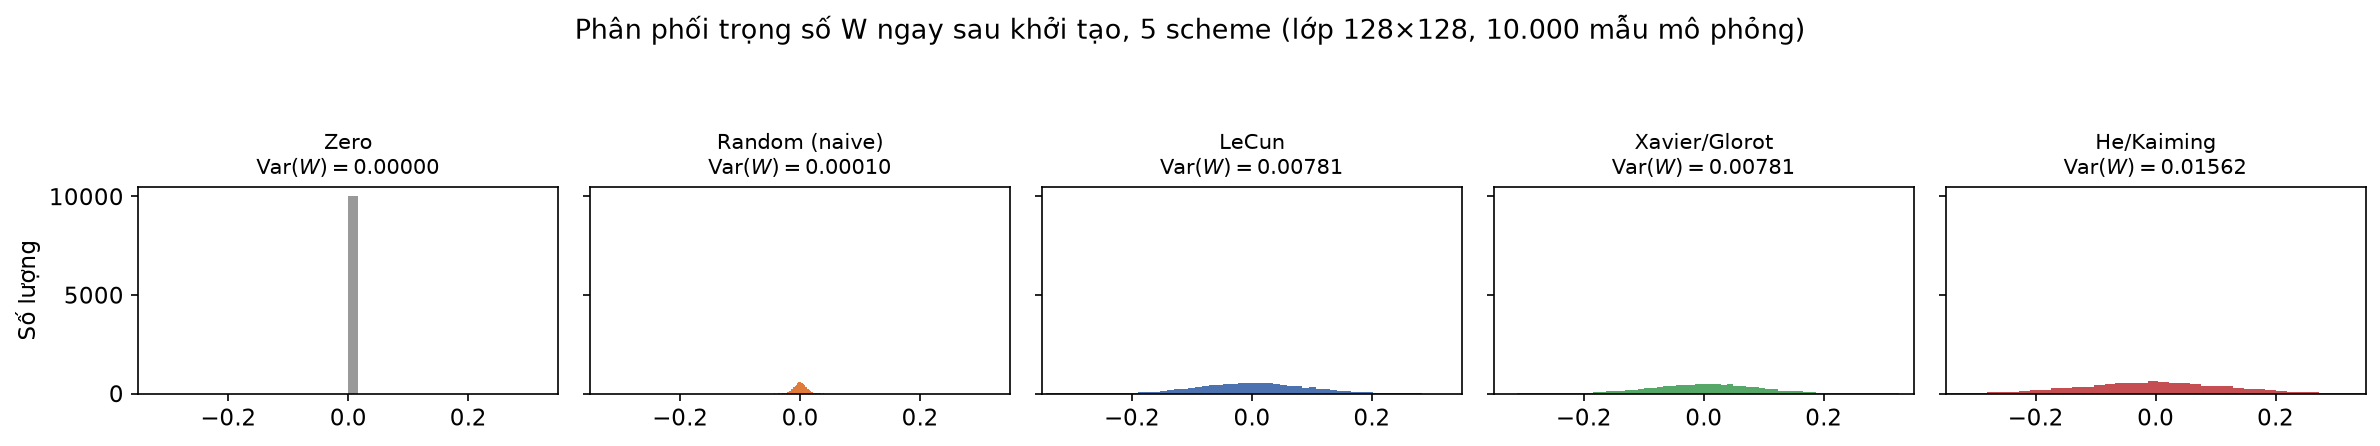
\includegraphics[width=0.98\linewidth]{figures/weight_init_histogram.png}
\caption{Phân phối $10\,000$ giá trị $W$ mô phỏng ngay sau khởi tạo theo
từng scheme (lớp $128\times128$, khớp $n_{\text{in}}{=}n_{\text{out}}{=}128$
của kiến trúc thực nghiệm Mục~\ref{sec:methodology}) --- Zero co về một
điểm; độ rộng phân phối tăng dần Random $<$ LeCun $=$ Xavier (khi
$n_{\text{in}}{=}n_{\text{out}}$) $<$ He, đúng thứ tự $\mathrm{Var}(W)$ ở
Bảng~\ref{tab:schemes}.}
\label{fig:weighthist}
\end{figure}

\textbf{Vì sao He nhân đôi so với LeCun?} ReLU đặt khoảng một nửa output
về $0$ (phần $z<0$), nên với $z$ đối xứng quanh $0$:
$\mathrm{Var}(\mathrm{ReLU}(z)) \approx \tfrac12\mathrm{Var}(z)$ --- để bù
phần ``mất'' này, \citet{he2015delving} nhân đôi variance của $W$ so với
công thức forward-preserving thuần ($1/n_{\text{in}}$) để giữ
$\mathrm{Var}(a)\approx\mathrm{Var}(x)$ qua mỗi lớp ReLU.

\textbf{Hệ quả thứ hai của ReLU: lệch tâm dương (positive mean shift).}
Phân tích variance ở trên chỉ kiểm soát \emph{bậc hai} (variance) của tín
hiệu; ReLU còn tạo ra một hiệu ứng \emph{bậc một} (kỳ vọng) mà công thức
$\mathrm{Var}(W)=2/n_{\text{in}}$ \textbf{không} khắc phục. Vì
$\mathrm{ReLU}(z)=\max(0,z)\ge0$ với mọi $z$, và với giả thiết chuẩn
$z\sim\mathcal N(0,\sigma_z^2)$ (dùng xuyên suốt Mục~\ref{sec:schemes}):
$$\mathbb E[\mathrm{ReLU}(z)] = \int_0^\infty z\,\frac{1}{\sigma_z\sqrt{2\pi}}e^{-z^2/2\sigma_z^2}\,dz = \frac{\sigma_z}{\sqrt{2\pi}} \approx 0.40\,\sigma_z \;>\;0.$$
Nói cách khác, \textbf{đầu ra trung bình của mỗi neuron ReLU luôn dương},
bất kể trọng số $W$ có kỳ vọng $0$ (đối xứng) hay không --- khác hẳn
Tanh/Sigmoid-đã-chuẩn-hoá vốn có $\mathbb E[a]\approx0$. Hệ quả: input của
lớp kế tiếp không còn ``căn giữa'' quanh $0$ như giả thiết ngầm trong mọi
phân tích $\mathrm{Var}(z)=n_{\text{in}}\mathrm{Var}(W)\mathrm{Var}(x)$ ở
Mục~\ref{sec:schemes} (vốn coi $x$ có kỳ vọng $0$) --- input không căn
giữa là chính xác dạng vấn đề mà \citet{lecun1998efficient} đã chỉ ra làm
xấu điều kiện (\en{conditioning}) của bề mặt tối ưu và làm chậm hội tụ
(phân tích gốc cho \emph{input} của mạng, nhưng áp dụng y hệt cho input
của \emph{mọi lớp ẩn} khi lớp trước là ReLU). Qua nhiều lớp liên tiếp,
lệch tâm dương ở mỗi lớp \emph{cộng dồn} về mặt hiệu ứng lên độ xấu điều
kiện tổng thể, dù bản thân variance vẫn được He initialization giữ ổn
định.

\begin{tructiep}[Vì sao có ELU, SELU]
Lệch tâm dương của ReLU là động lực trực tiếp cho các activation ``đã sửa
tâm'' ra đời sau đó: \textbf{ELU} (\en{Exponential Linear Unit})
--- $\mathrm{ELU}(z)=z$ nếu $z>0$, $\alpha(e^z-1)$ nếu $z\le0$
--- bão hoà về $-\alpha$ (thay vì cắt cứng về $0$ như ReLU) ở nhánh âm,
kéo $\mathbb E[a]$ về gần $0$ hơn~\citep{clevert2016elu}. \textbf{SELU}
(\en{Scaled ELU}) đẩy ý tưởng này xa hơn: chọn đúng hai hằng số
$\lambda,\alpha$ sao cho phép lặp forward qua nhiều lớp tự động hội tụ
kỳ vọng về $0$ và variance về $1$ --- gọi là tính chất
\textbf{tự chuẩn hoá} (\en{self-normalizing})~\citep{klambauer2017selu}.
Kiến trúc thực nghiệm của báo cáo này (Mục~\ref{sec:methodology}) chỉ
dùng Sigmoid/Tanh/ReLU/Leaky ReLU, không thử ELU/SELU --- nêu ở đây để
định vị đúng vị trí của He initialization trong dòng phát triển: giải
quyết vấn đề \emph{variance}, còn vấn đề \emph{mean shift} được các kiến
trúc activation sau đó giải quyết theo hướng khác.
\end{tructiep}

\textbf{Vì sao Xavier lấy trung bình $n_{\text{in}}$ và $n_{\text{out}}$?}
Phân tích forward (giữ $\mathrm{Var}(z)$) cho $\mathrm{Var}(W)=1/n_{\text{in}}$;
phân tích backward (giữ $\mathrm{Var}(\partial L/\partial a)$ khi lan
truyền ngược) cho $\mathrm{Var}(W)=1/n_{\text{out}}$. Hai điều kiện này chỉ
trùng nhau khi $n_{\text{in}}=n_{\text{out}}$ (hiếm khi đúng trong thực
tế); \citet{glorot2010understanding} chọn điểm dung hoà
$\mathrm{Var}(W)=2/(n_{\text{in}}+n_{\text{out}})$ để không hy sinh hẳn
điều kiện nào.

\textbf{Bias}: cả 3 scheme trên đều khởi tạo $b=0$ --- bias không gây vấn
đề đối xứng \emph{giữa các neuron} theo cùng cách $W$ gây ra (mỗi $b_j$
vẫn có thể học giá trị khác nhau miễn $W$ đã phá đối xứng), nên giữ $b=0$
là điểm khởi đầu trung tính, đơn giản, được dùng thống nhất trong toàn bộ
thực nghiệm của báo cáo (Mục~\ref{sec:methodology}).

\begin{tructiep}[Biến thể: bias dương nhỏ cho ReLU]
Một số tài liệu thực hành (không dùng trong thực nghiệm của báo cáo này,
nêu ở đây để đầy đủ) đề xuất khởi tạo $b$ bằng một hằng số dương nhỏ, ví
dụ $b=0.01$, thay vì $0$ cho các lớp dùng ReLU. Lý do: nếu $z=W\T x+b<0$
ngay ở bước forward đầu tiên (trước khi $W$ kịp học), neuron đó rơi vào
trạng thái $\mathrm{ReLU}(z)=0$ và $\mathrm{ReLU}'(z)=0$ --- không có
gradient chảy qua để cập nhật $W,b$, tức nguy cơ \emph{dead ReLU} ngay từ
lúc khởi tạo. Một độ lệch dương nhỏ trong $b$ đẩy nhiều neuron hơn về phía
$z>0$ lúc khởi đầu, giảm xác suất "chết" sớm. Đánh đổi: $b>0$ phá vỡ tính
trung tính của bias và có thể làm lệch phân phối activation ban đầu; đây
là lý do thực nghiệm của báo cáo giữ $b=0$ để tách biệt hoàn toàn hiệu ứng
của $\mathrm{Var}(W)$ (biến độc lập đang khảo sát) khỏi hiệu ứng phụ của
bias.
\end{tructiep}

\subsection{Chuỗi ảnh hưởng: Initialization $\to$ Training Stability}

\begin{align*}
\text{Initialization }(\mathrm{Var}(W)) \;&\Rightarrow\; \text{Activation variance qua mỗi lớp} \\
&\Rightarrow\; \text{Gradient variance khi lan truyền ngược} \\
&\Rightarrow\; \text{Ổn định huấn luyện.}
\end{align*}
Nếu mỗi lớp nhân variance tín hiệu với hệ số $r=n_{\text{in}}\,\mathrm{Var}(W)$
(bỏ qua hiệu chỉnh riêng của activation), sau $L$ lớp:
$\mathrm{Var}(a^{(L)}) \approx r^L\cdot\mathrm{Var}(x)$ --- \textbf{tăng
hoặc giảm theo hàm mũ của độ sâu} nếu $r\ne1$. Đây chính là cơ chế toán
học của vanishing/exploding gradient, trình bày chi tiết ở Mục~\ref{sec:vanishing}.

\subsection{Ví dụ số: lan truyền variance qua nhiều lớp}
\label{sec:varprop}

Áp công thức $r=n_{\text{in}}\mathrm{Var}(W)$ (đã hiệu chỉnh cho từng
activation) vào kiến trúc thực tế của báo cáo
($n_{\text{in}}=128$ cho mọi lớp ẩn, xem Mục~\ref{sec:methodology}),
giả sử $\mathrm{Var}(x)=1$ ở đầu vào lớp ẩn đầu tiên (Bảng~\ref{tab:varprop}
--- tính lý tưởng hoá, bỏ qua hiệu ứng bão hoà thực tế của activation;
số liệu \emph{đo được thật} trên mạng thật nằm ở Hình~\ref{fig:actvar},
\ref{fig:wvar} Mục~\ref{sec:results}):

\begin{table}[H]
\centering
\caption{$\mathrm{Var}(a^{(l)})$ lý thuyết theo độ sâu $l$, ba scheme minh hoạ ($n_{\text{in}}=128$)}
\footnotesize
\begin{tabular}{@{}lccccccc@{}}
\toprule
Scheme & $l{=}0$ & $l{=}1$ & $l{=}2$ & $l{=}3$ & $l{=}4$ & $l{=}5$ & $l{=}6$ \\
\midrule
He+ReLU & $1.00$ & $1.00$ & $1.00$ & $1.00$ & $1.00$ & $1.00$ & $1.00$ \\
Xavier+Tanh & $1.00$ & $1.00$ & $1.00$ & $1.00$ & $1.00$ & $1.00$ & $1.00$ \\
Random & $1.00$ & $1.28\text{e-}2$ & $1.64\text{e-}4$ & $2.10\text{e-}6$ & $2.68\text{e-}8$ & $3.44\text{e-}10$ & $4.40\text{e-}12$ \\
\bottomrule
\end{tabular}
\label{tab:varprop}
\end{table}
\emph{Ghi chú}: hệ số nhân dồn mỗi lớp $r_{\text{eff}}\approx1$ cho hai
scheme đầu (theo thiết kế, Mục~\ref{sec:schemes}); $r=n_{\text{in}}\mathrm{Var}(W)=0.0128$
cho Random (naive, $\sigma=0.01$ cố định, không hiệu chỉnh activation).

Với He/Xavier, hệ số $r$ được \emph{thiết kế} để xấp xỉ $1$ nên variance
tín hiệu giữ nguyên bậc-độ-lớn qua cả 6 lớp. Với Random (naive)
($\sigma=0.01$ cố định $\Rightarrow r=128\times0.01^2=0.0128$),
variance suy giảm \textbf{10 bậc độ lớn} chỉ sau 6 lớp --- khớp đúng bậc
độ lớn với suy giảm gradient đo được thật trong Hình~\ref{fig:gradnorm}
($\approx$9 bậc từ lớp 7 về lớp 1), vì gradient và activation suy giảm
theo cùng cơ chế nhân dồn (Mục~\ref{sec:vanishing}).

\subsection{Activation × Initialization: bảng tương thích}

Bảng~\ref{tab:compat} tóm tắt khuyến nghị lý thuyết; Mục~\ref{sec:results}
kiểm chứng bằng lưới thực nghiệm đầy đủ $5\times4=20$ cấu hình --- \textbf{không
phải mọi khuyến nghị lý thuyết đều thành công như nhau trong thực nghiệm
CPU/dữ liệu nhỏ của báo cáo này} (xem Mục~\ref{sec:discussion}).

\begin{table}[H]
\centering
\caption{Khuyến nghị lý thuyết Activation $\times$ Initialization (không phải quy tắc tuyệt đối)}
\begin{tabular}{@{}lp{10.5cm}@{}}
\toprule
\textbf{Activation} & \textbf{Initialization phù hợp và lý do} \\
\midrule
Sigmoid & Xavier/LeCun --- hàm đối xứng quanh $0.5$, nhưng $\sigma'(z)\le0.25$ luôn luôn nên vẫn dễ vanishing ở mạng sâu \emph{dù} initialization đúng (Mục~\ref{sec:vanishing}) \\
Tanh & Xavier --- đối xứng quanh $0$, đạo hàm cực đại $=1$ tại $z=0$, ít suy giảm hơn Sigmoid đáng kể \\
ReLU & He/Kaiming --- bù trực tiếp việc ReLU triệt tiêu $\approx$ một nửa variance \\
Leaky ReLU & He/Kaiming (gần đúng) --- tương tự ReLU, phần âm không hoàn toàn triệt tiêu nên ít ``dead neuron'' hơn \\
\bottomrule
\end{tabular}
\label{tab:compat}
\end{table}

%==============================================================================
% 6. VANISHING / EXPLODING GRADIENT
%==============================================================================
\section{Vanishing và Exploding Gradient}
\label{sec:vanishing}

Theo Chain Rule, gradient tại lớp đầu là \textbf{tích} của nhiều đạo hàm
cục bộ dọc theo $L$ lớp:
$$\frac{\partial L}{\partial a^{(0)}} = \frac{\partial L}{\partial a^{(L)}}\prod_{l=1}^{L} \frac{\partial a^{(l)}}{\partial a^{(l-1)}}.$$
Nếu độ lớn trung bình mỗi nhân tử cục bộ $\approx g$:
\begin{itemize}
\item $g<1$: tích $\approx g^L \to 0$ theo hàm mũ khi $L$ tăng ---
  \textbf{vanishing gradient}: lớp đầu gần như không nhận được tín hiệu
  học.
\item $g>1$: tích $\approx g^L \to \infty$ --- \textbf{exploding
  gradient}: bước cập nhật quá lớn, loss dao động hoặc \texttt{NaN}.
\item $g=1$: tích ổn định ở mọi độ sâu --- mục tiêu mà Xavier/He hướng
  tới (Mục~\ref{sec:schemes}).
\end{itemize}

\begin{table}[H]
\centering
\caption{Minh hoạ số: hệ số nhân dồn $g^L$ theo độ sâu $L$ (đã tính lại
bằng \url{experiments/toy_example_verify.py})}
\begin{tabular}{@{}lccccc@{}}
\toprule
$g$ & $L=1$ & $L=5$ & $L=10$ & $L=20$ & $L=50$ \\
\midrule
$0.5$ (vanishing) & $5.0\times10^{-1}$ & $3.1\times10^{-2}$ & $9.8\times10^{-4}$ & $9.5\times10^{-7}$ & $8.9\times10^{-16}$ \\
$1.0$ (ổn định) & $1.0$ & $1.0$ & $1.0$ & $1.0$ & $1.0$ \\
$2.0$ (exploding) & $2.0$ & $3.2\times10^{1}$ & $1.0\times10^{3}$ & $1.0\times10^{6}$ & $1.1\times10^{15}$ \\
\bottomrule
\end{tabular}
\label{tab:ge_numeric}
\end{table}

Với $g=0.5$, sau $L=10$ lớp hệ số chỉ còn $\approx1/1024$; sau $L=50$ lớp
gần như bằng $0$ dưới độ chính xác số thực. Với $g=2$, sau $L=10$ lớp hệ số
đã là $1024$; sau $L=50$ là hơn $10^{15}$. Bảng~\ref{tab:ge_numeric} minh
hoạ trực quan vì sao ``giữ $g\approx1$'' (chính là mục tiêu của Xavier/He)
quan trọng với mạng sâu --- một sai lệch nhỏ ở $g$ bị \textbf{khuếch đại
theo hàm mũ} của số lớp.

$g$ phụ thuộc \textbf{cả ba yếu tố}: activation (hệ số co từ đạo hàm $f'$
--- vd. $\sigma'(z)\le0.25$ luôn luôn co lại), weight scale (qua
$\mathrm{Var}(W)$, Mục~\ref{sec:schemes}), và độ sâu $L$ (số lần nhân).
Thực nghiệm Mục~\ref{sec:results} (Hình~\ref{fig:gradnorm}) đo trực tiếp
gradient theo từng lớp trên mạng thật, xác nhận đúng ba yếu tố này cùng
tác động.

\begin{tructiep}[Vì sao ReLU giúp giảm vanishing so với Sigmoid/Tanh]
$\mathrm{ReLU}'(z)\in\{0,1\}$ (tại $z=0$, xem quy ước dưới đạo hàm
Mục~\ref{sec:compgraph}) --- khi ``sống'' ($z>0$), hệ số nhân đúng bằng
$1$ (không co lại như $\sigma'(z)\le0.25$); khi ``chết'' ($z\le0$), hệ số
bằng $0$ hoàn toàn (không ``biến mất dần'' mà ``cắt đứt hẳn''). Đây là lý do
ReLU không bị vanishing \emph{do chính activation gây ra} như Sigmoid,
nhưng đổi lại có rủi ro riêng: \textbf{dead ReLU} (neuron chết vĩnh viễn
nếu rơi vào vùng $z\le0$ và không bao giờ nhận gradient để ``sống lại''
--- đã thấy trong ví dụ Bảng~\ref{tab:2layer_numeric}).
\end{tructiep}

\subsection{Thực nghiệm bổ sung: độ sâu ảnh hưởng thế nào tới initialization}
\label{sec:depthexp}

Lưới $20$ cấu hình chính (Mục~\ref{sec:results}) cố định độ sâu $=6$ lớp
ẩn. Để kiểm chứng trực tiếp dự đoán lý thuyết của mục này ---
\emph{``vanishing/exploding trầm trọng hơn theo hàm mũ của độ sâu''} --- nhóm
chạy thêm một thực nghiệm riêng (\url{experiments/run_depth_experiment.py}):
so sánh \textbf{He} và \textbf{Random (naive)}, activation ReLU, tại
\textbf{6 độ sâu khác nhau} $L\in\{2,4,6,8,10,12\}$ lớp ẩn (rộng cố định
$128$), đo (a) gradient RMS lớp $1$ \emph{ngay tại bước khởi tạo} (không
cần huấn luyện, đo nhanh và tách bạch khỏi hiệu ứng optimizer) và (b) test
accuracy sau $8$ epoch huấn luyện thật (rút ngắn so với $15$ epoch của
lưới chính để tổng thời gian hợp lý với $6\times2=12$ cấu hình bổ sung).

\begin{figure}[H]
\centering
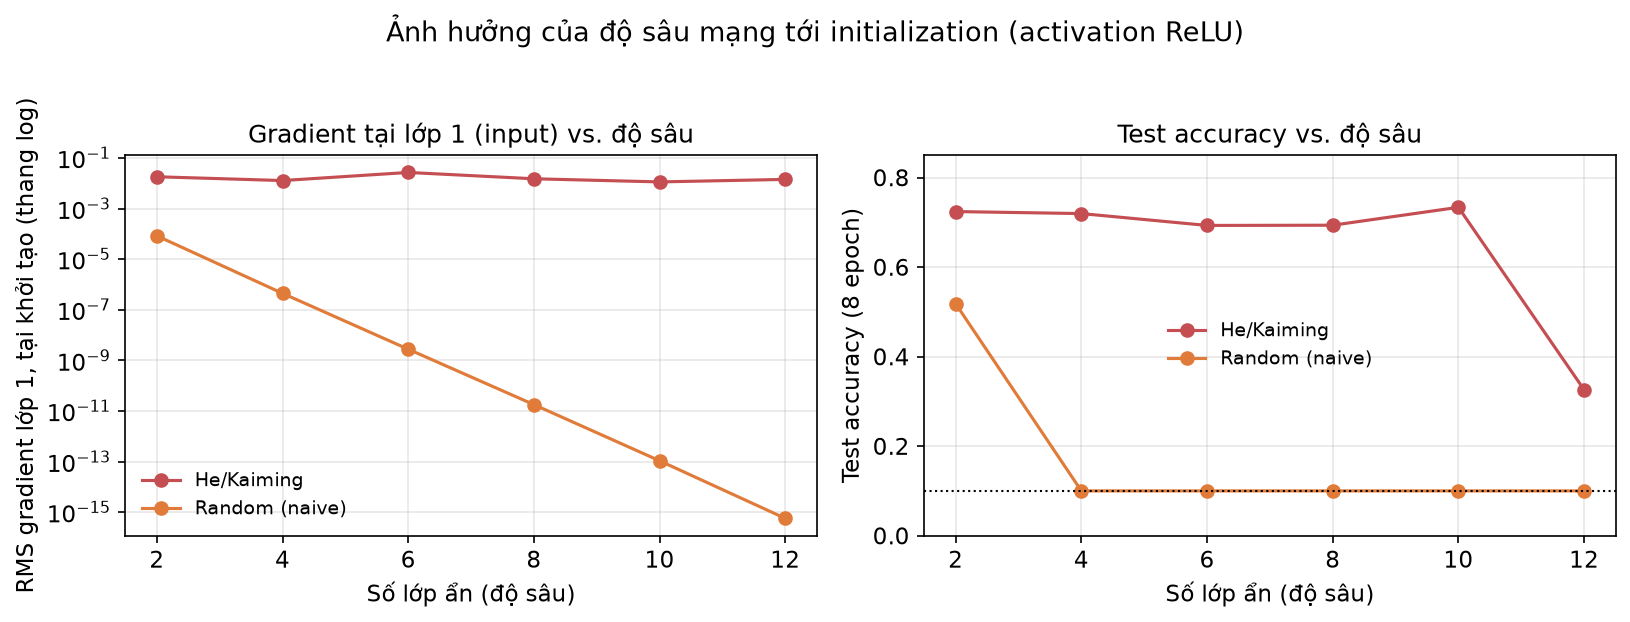
\includegraphics[width=0.95\linewidth]{figures/depth_experiment.png}
\caption{Gradient RMS lớp 1 tại khởi tạo (trái) và test accuracy sau 8
epoch (phải), theo độ sâu mạng, activation ReLU. Đường chấm ở đồ thị phải
= mức ngẫu nhiên ($10\%$).}
\label{fig:depthexp}
\end{figure}

\textbf{Ba quan sát chính} (Hình~\ref{fig:depthexp}):

\begin{enumerate}
\item \textbf{Random (naive) suy giảm gradient theo đúng đường thẳng trên
  thang log} khi độ sâu tăng tuyến tính --- từ $\approx8.3\times10^{-5}$
  ($L{=}2$) xuống $\approx5.7\times10^{-16}$ ($L{=}12$), tức
  \textbf{suy giảm 12 bậc độ lớn chỉ sau 10 lớp thêm vào} --- xác nhận
  trực tiếp mô hình $g^L$ (Mục~\ref{sec:vanishing}, Bảng~\ref{tab:ge_numeric}):
  trên thang log, $\log(g^L)=L\log g$ là một đường thẳng theo $L$, đúng
  như đồ thị cho thấy.
\item \textbf{Test accuracy của Random sụp xuống mức ngẫu nhiên ngay từ
  $L{=}4$} --- chỉ cần tăng độ sâu từ 2 lên 4 lớp là đủ để một
  initialization ``tạm chấp nhận được'' ở mạng nông ($52\%$ ở $L{=}2$, đã
  kém nhưng còn học được chút ít) trở thành hoàn toàn vô dụng.
\item \textbf{He giữ gradient ổn định (bậc $10^{-2}$) ở mọi độ sâu từ 2
  đến 12 lớp} --- kể cả tại $L{=}12$, đúng như thiết kế của
  Mục~\ref{sec:schemes}: gradient RMS lớp 1 tại khởi tạo vẫn bình thường
  ($\approx4\times10^{-2}$, Hình~\ref{fig:depthexp} trái, không hề suy
  giảm so với các độ sâu nhỏ hơn). Tuy nhiên, test accuracy tại $L{=}12$
  \textbf{giảm mạnh xuống $32.6\%$}. Đối chiếu \emph{cả hai} loss (không
  chỉ accuracy) loại trừ ngay giả thuyết vanishing gradient:
  train loss $=0.456$ (khớp fit tốt trên tập train, cùng bậc với mọi độ
  sâu khác --- $0.36$--$0.42$) trong khi test loss vọt lên
  $5.409$ --- \textbf{vượt xa} cả mức loss của một mô hình đoán ngẫu
  nhiên hoàn toàn ($-\ln(1/10)\approx2.303$). Một mô hình \emph{không
  học được gì} (vanishing gradient thực sự) sẽ có train loss \emph{và}
  test loss đều mắc kẹt gần $2.3$ như các cấu hình Zero/Random
  (Bảng~\ref{tab:results_grid}); ở đây train loss thấp chứng tỏ mô hình
  \emph{học được} trên tập train. Chữ ký số liệu này (train loss thấp,
  test loss cao hơn cả baseline ngẫu nhiên) là dấu hiệu kinh điển của
  \textbf{suy sụp năng lực khái quát hoá} (\en{generalization collapse}
  do overfitting), không phải vanishing gradient: một MLP $12$ lớp ẩn
  ($283\,402$ tham số, tính theo đúng công thức Mục~\ref{sec:complexity})
  huấn luyện trên vỏn vẹn $5\,000$ mẫu, không regularization, dễ dàng ghi
  nhớ (\en{memorize}) nhiễu của tập train thay vì học đặc trưng tổng
  quát --- và vì không có softmax/Cross-Entropy nào ``giới hạn'' độ tự
  tin sai, một dự đoán sai với xác suất gần $1$ cho loss cực lớn (xem
  công thức Cross-Entropy Mục~\ref{sec:softmax}: $L=-\log p_{y}$ tiến tới
  $\infty$ khi $p_y\to0$). \textbf{Kết luận methodological quan trọng}:
  Var(W) đúng theo He/Kaiming đảm bảo tín hiệu/gradient \emph{tại khởi
  tạo}, nhưng không kiểm soát được năng lực khái quát hoá trong suốt quá
  trình huấn luyện --- hai vấn đề tách biệt, không nên gộp chung (thảo
  luận đầy đủ ở Mục~\ref{sec:limitations}).
\end{enumerate}

%==============================================================================
% 7. EXPERIMENTAL METHODOLOGY
%==============================================================================
\section{Phương pháp thực nghiệm}
\label{sec:methodology}

\textbf{Mục tiêu}: kiểm chứng bằng số liệu thật (không minh hoạ suông) ba
dự đoán lý thuyết của Mục~\ref{sec:init}--\ref{sec:vanishing}: (a) Zero/Random
(naive) không học được; (b) initialization có scale đúng (LeCun/Xavier/He)
học tốt hơn rõ rệt; (c) gradient theo từng lớp thể hiện đúng mẫu
vanishing/exploding dự đoán bởi lý thuyết.

\subsection{Dataset và tiền xử lý}
\label{sec:dataset}

\textbf{Fashion-MNIST}~\citep{xiao2017fashionmnist} qua \texttt{torchvision}:
ảnh $28\times28$ xám, 10 lớp trang phục, cân bằng số lượng giữa các lớp.
Chọn thay MNIST chữ số thuần vì MNIST quá dễ (một MLP nông cũng đạt
$>97\%$), làm mờ tác động của initialization đang muốn khảo sát;
Fashion-MNIST khó hơn vừa đủ để 5 scheme initialization tạo ra khác biệt
rõ ràng mà vẫn đủ nhẹ để chạy nhanh trên CPU.

\begin{figure}[H]
\centering
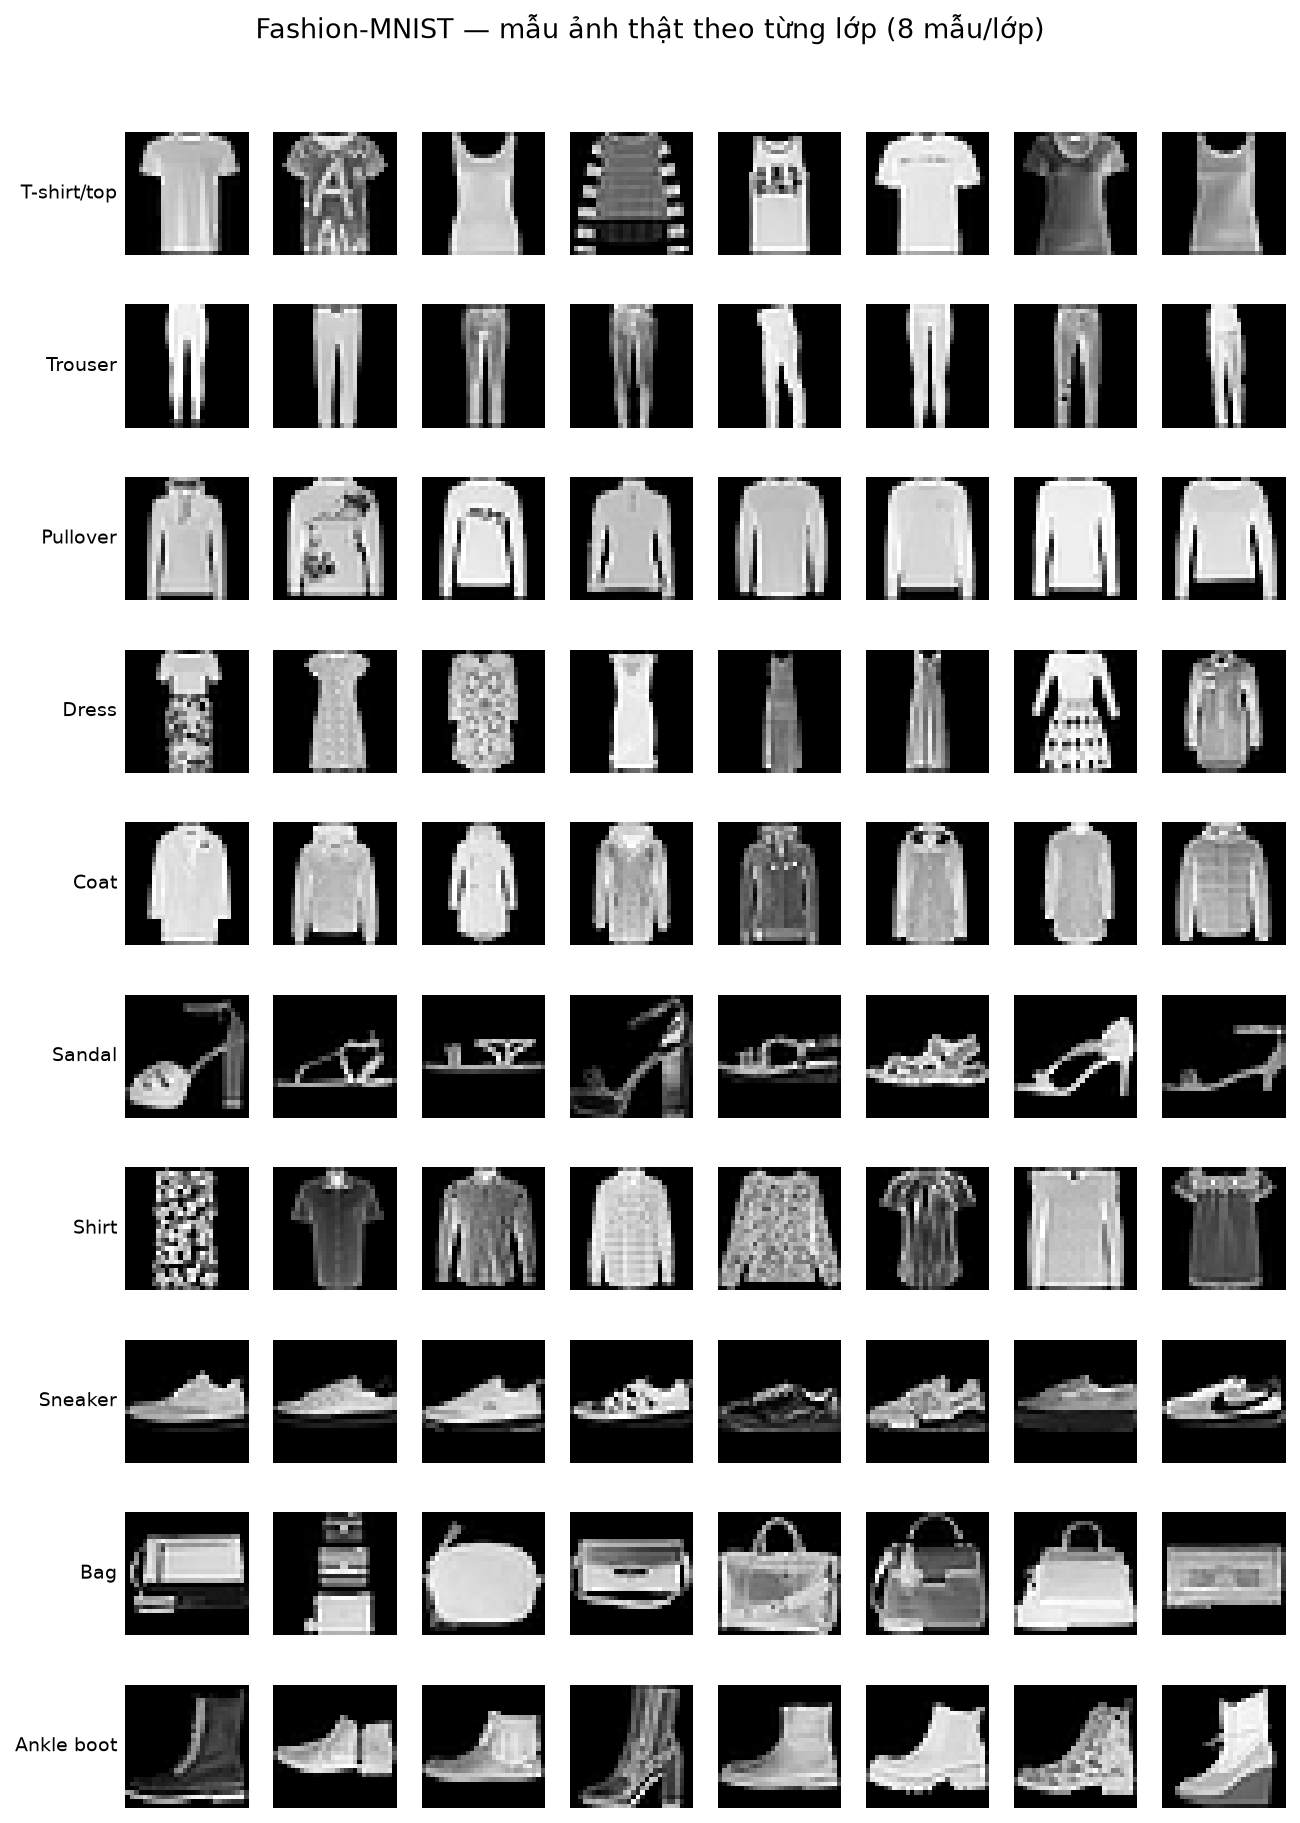
\includegraphics[width=0.62\linewidth]{figures/fashion_mnist_samples.png}
\caption{Mẫu ảnh thật của cả 10 lớp Fashion-MNIST (8 mẫu/lớp, lấy ngẫu
nhiên từ tập train đang dùng).}
\label{fig:samples}
\end{figure}

\begin{table}[H]
\centering
\caption{10 lớp của Fashion-MNIST}
\small
\begin{tabular}{@{}cl@{\hspace{1.2cm}}cl@{\hspace{1.2cm}}cl@{}}
\toprule
0 & T-shirt/top & 4 & Coat & 8 & Bag \\
1 & Trouser & 5 & Sandal & 9 & Ankle boot \\
2 & Pullover & 6 & Shirt & & \\
3 & Dress & 7 & Sneaker & & \\
\bottomrule
\end{tabular}
\label{tab:classes}
\end{table}

\textbf{Subset để chạy nhanh trên CPU} (khai báo minh bạch, không giấu):
$5\,000$ mẫu train / $1\,000$ val / $2\,000$ test, lấy ngẫu nhiên
\emph{cân bằng theo lớp} (\en{stratified sampling} --- mỗi lớp góp số
mẫu bằng nhau, tránh lệch phân phối khi cắt subset từ $60\,000$ mẫu gốc),
seed cố định $=42$.

\textbf{Tiền xử lý}: mỗi ảnh làm phẳng thành vector $784$ chiều
($28\times28\to784$, khớp input của MLP, Mục~\ref{sec:forward}), giá trị
pixel gốc $\in[0,255]$ chia $255$ về $[0,1]$, sau đó chuẩn hoá
$(\text{pixel}-\mu)/\sigma$ với $\mu=0.2881$, $\sigma=0.3543$ ---
\textbf{tính trực tiếp từ chính $5\,000$ mẫu train đang dùng} (không tra
số liệu chuẩn hoá từ nguồn khác) để tránh rò rỉ thông tin từ phần dữ liệu
không dùng tới huấn luyện.

\subsection{Kiến trúc mô hình}
\label{sec:architecture}

MLP 6 hidden layer, \textbf{cố định cho mọi cấu hình}, không
BatchNorm/Dropout, không pretrained:
$$784 \to 128 \to 128 \to 128 \to 128 \to 128 \to 128 \to 10.$$
Lớp output luôn linear (logits), dùng \texttt{CrossEntropyLoss} (softmax
nằm trong hàm loss). Độ sâu 6 lớp ẩn được chọn \textbf{cố ý đủ sâu} để
chênh lệch giữa các initialization thể hiện rõ (một MLP 1--2 lớp gần như
không nhạy với initialization, xem thảo luận Mục~\ref{sec:discussion}) mà
vẫn huấn luyện nhanh trên CPU.

\subsection{Thiết kế lưới thực nghiệm}
\label{sec:designgrid}

\textbf{Biến thực nghiệm (fair experiment)}: lưới đầy đủ
$5\text{ initialization}\times4\text{ activation}=20$ cấu hình
(Bảng~\ref{tab:grid}) --- \emph{chỉ} initialization và activation thay
đổi; kiến trúc, optimizer, learning rate, batch size, epoch, seed, cách
chia dữ liệu giống hệt nhau giữa 20 lần chạy.

\begin{table}[H]
\centering
\caption{Lưới thực nghiệm $5\times4=20$ cấu hình (Experiment 1--8 đều rút ra từ lưới này)}
\begin{tabular}{@{}lcccc@{}}
\toprule
 & Sigmoid & Tanh & ReLU & Leaky ReLU \\
\midrule
Zero & \checkmark & \checkmark & \checkmark & \checkmark \\
Random (naive) & \checkmark & \checkmark & \checkmark & \checkmark \\
LeCun & \checkmark & \checkmark & \checkmark & \checkmark \\
Xavier/Glorot & \checkmark & \checkmark & \checkmark & \checkmark \\
He/Kaiming & \checkmark & \checkmark & \checkmark & \checkmark \\
\bottomrule
\end{tabular}
\label{tab:grid}
\end{table}

Ánh xạ sang 8 experiment theo đề cương: Exp.\ 1--5 (Zero/Random/LeCun/Xavier/He)
= cột \textbf{ReLU}; Exp.\ 6 (so sánh activation) = hàng \textbf{He} và
hàng \textbf{Xavier}; Exp.\ 7 (gradient norm theo layer) = lát cắt
\textbf{Sigmoid} (nơi vanishing rõ nhất về lý thuyết); Exp.\ 8 (training
convergence) = loss/accuracy theo epoch của chính 20 lần chạy trên.

\begin{table}[H]
\centering
\caption{Siêu tham số cố định cho toàn bộ 20 cấu hình}
\begin{tabular}{@{}ll@{}}
\toprule
Optimizer & SGD thuần (không momentum) \\
Learning rate $\eta$ & $0.05$ \\
Batch size & $128$ \\
Epochs & $15$ \\
Seed & $42$ (Python, NumPy, PyTorch) \\
Bias init & $0$ (mọi scheme) \\
Loss & CrossEntropyLoss \\
\bottomrule
\end{tabular}
\label{tab:hparams}
\end{table}

SGD thuần (không Adam) được chọn \textbf{cố ý}: optimizer thích ứng
(adaptive) như Adam có learning rate riêng cho từng tham số, có thể che
bớt một phần ảnh hưởng của initialization kém --- dùng SGD thuần để quan
sát đúng hiệu ứng lý thuyết Mục~\ref{sec:init}--\ref{sec:vanishing}, đánh
đổi lấy khả năng hội tụ chậm hơn/không ổn định hơn ở một số cấu hình (thảo
luận ở Mục~\ref{sec:limitations}).

\subsection{Metric thu thập}

\textbf{Metric thu thập}: mỗi epoch --- train/val loss, train/val
accuracy; tại \textbf{bước đầu tiên} (trước update đầu tiên) --- gradient
RMS theo từng lớp, activation mean/variance theo từng lớp, weight
mean/variance theo từng lớp, cùng một mẫu gradient/activation thô ở lớp
giữa mạng (để vẽ histogram).

\textbf{Vì sao dùng RMS thay vì norm thô để so sánh giữa các lớp?} Lớp 1
($784\to128$) có $100\,352$ phần tử $W$, các lớp ẩn giữa ($128\to128$)
chỉ có $16\,384$ --- so trực tiếp $\lVert\partial L/\partial W\rVert_2$
(norm Frobenius thô) giữa hai lớp này bị lệch chỉ vì kích thước ma trận
khác nhau, không phản ánh đúng "độ lớn gradient mỗi trọng số". Báo cáo
dùng \textbf{RMS} (\en{root-mean-square}), chuẩn hoá theo số phần tử:
$$\mathrm{RMS}\Big(\frac{\partial L}{\partial W^{(l)}}\Big) = \frac{\lVert\partial L/\partial W^{(l)}\rVert_2}{\sqrt{|W^{(l)}|}}$$
($|W^{(l)}|$ = tổng số phần tử của $W^{(l)}$) --- đây chính là đại lượng
vẽ trong Hình~\ref{fig:gradnorm}, \ref{fig:depthexp}, cho phép so sánh
công bằng giữa các lớp có kích thước khác nhau (chi tiết cài đặt: hàm
\texttt{grad\_norms\_per\_layer} trong \url{src/metrics.py}).

\subsection{Môi trường tính toán (System Environment)}
\label{sec:sysenv}

Để phục vụ tái lập kết quả (\en{reproducibility}), Bảng~\ref{tab:sysenv}
liệt kê đầy đủ cấu hình phần cứng và phiên bản phần mềm dùng để chạy toàn
bộ thực nghiệm của báo cáo.

\begin{table}[H]
\centering
\caption{Cấu hình môi trường thực nghiệm}
\small
\begin{tabular}{@{}ll@{}}
\toprule
\textbf{Thành phần} & \textbf{Chi tiết} \\
\midrule
CPU & Intel Core i5-13420H (13th Gen) \\
RAM & 16 GB \\
GPU & Không dùng --- toàn bộ thực nghiệm chạy trên CPU \\
Hệ điều hành & Windows 11 (build 10.0.26200) \\
Python & 3.11.9 \\
PyTorch & 2.14.0+cpu \\
NumPy & 2.4.6 \\
\bottomrule
\end{tabular}
\label{tab:sysenv}
\end{table}

Vì kiến trúc mô hình nhỏ (Mục~\ref{sec:architecture}) và dataset đã được
lấy mẫu con còn $5\,000$ ảnh (Mục~\ref{sec:dataset}), toàn bộ $20$ cấu
hình của lưới thực nghiệm chính (Mục~\ref{sec:designgrid}) chạy hoàn toàn
trên CPU trong thời gian hợp lý, không cần GPU/CUDA --- một lựa chọn có
chủ đích để giữ bài toán trong tầm tái lập trên phần cứng phổ thông (xem
thêm Mục~\ref{sec:limitations} về đánh đổi giữa quy mô thực nghiệm và tốc
độ lặp).

%==============================================================================
% 8. IMPLEMENTATION
%==============================================================================
\section{Hiện thực}
\label{sec:implementation}

Mã nguồn đầy đủ nằm trong \texttt{src/} (module hoá) và
\texttt{experiments/} (script chạy) --- xem cấu trúc trong
\texttt{README.md}. Hai phần quan trọng nhất:

\subsection{Part A: Manual Backpropagation}

\textbf{Part A --- Manual Backpropagation} (\texttt{src/manual\_nn.py}):
forward/backward tự viết bằng NumPy thuần, \textbf{không dùng autograd},
triển khai đúng công thức Mục~\ref{sec:matrixform}:

\begin{lstlisting}[caption={Backward pass thủ công (trích từ src/manual\_nn.py)}]
dA = (Yhat - Y) / N          # dL/dA^(L)
for l in reversed(range(n_layers)):
    is_last = (l == n_layers - 1)
    dZ = dA if is_last else dA * f_grad(Zs[l])
    grads_W[l] = As[l].T @ dZ      # A^(l-1)^T dZ^(l)
    grads_b[l] = dZ.sum(axis=0)    # tong theo truc batch
    dA = dZ @ W[l].T               # dL/dA^(l-1)
\end{lstlisting}

\textbf{Phạm vi có chủ đích của Part A, và ranh giới rõ ràng với Part B.}
\texttt{ManualMLP} dùng hàm mất mát \textbf{MSE} (không phải
Cross-Entropy) và kiến trúc thu nhỏ tuỳ ý (vài chục neuron, xem các ví dụ
số Mục~\ref{sec:scalar}--\ref{sec:matrixform}) --- đây là lựa chọn
\emph{có chủ đích}, không phải giản lược tuỳ tiện: mục tiêu duy nhất của
Part A là \textbf{kiểm chứng số học độc lập} (\en{toy numerical
verification}) rằng công thức Chain Rule tự viết tay khớp chính xác với
PyTorch autograd và finite-difference (Mục~\ref{sec:gradcheck}) trên
những trường hợp đủ nhỏ để tính tay/kiểm tra bằng mắt được từng bước ---
\textbf{không} nhằm huấn luyện một mô hình thật. Việc huấn luyện thật,
trên bài toán phân loại $10$ lớp Fashion-MNIST với Softmax + Cross-Entropy
(Mục~\ref{sec:softmax}) và kiến trúc đủ sâu để initialization tạo khác
biệt ($784\to128^{\times L}\to10$, Mục~\ref{sec:methodology}), là công
việc của \textbf{Part B} dưới đây --- hai phần bổ trợ nhau chứ không thay
thế nhau: Part A chứng minh \emph{tính đúng đắn} của cơ chế backprop ở
quy mô kiểm tra được; Part B áp dụng chính cơ chế đó (qua autograd, đã
được Part A xác nhận là tương đương) ở quy mô đủ lớn để trả lời câu hỏi
nghiên cứu chính của báo cáo.

\subsection{Part B: PyTorch Autograd}

\textbf{Part B --- PyTorch Autograd} (\texttt{src/models.py},
\texttt{src/training.py}): kiến trúc tương đương dùng \texttt{torch.nn},
gradient tính bằng \texttt{loss.backward()} --- cơ chế \en{automatic
differentiation} của PyTorch~\citep{paszke2019pytorch}, về bản chất cũng
là Backpropagation (Mục~\ref{sec:backprop}) nhưng tự động xây và duyệt
computational graph thay vì viết tay như Part A; dùng cho toàn bộ 20 cấu
hình thực nghiệm chính (Mục~\ref{sec:methodology}) vì cần training thật
trên Fashion-MNIST, không khả thi bằng NumPy thuần trong phạm vi báo cáo.

\begin{lstlisting}[caption={Định nghĩa MLP và khởi tạo lại theo scheme (trích từ src/models.py)}]
class MLP(nn.Module):
    def __init__(self, input_dim=784, hidden_dims=None,
                 output_dim=10, activation="relu"):
        super().__init__()
        hidden_dims = hidden_dims or [128] * 6
        dims = [input_dim] + list(hidden_dims)
        self.linears = nn.ModuleList(
            [nn.Linear(dims[i], dims[i+1]) for i in range(len(dims)-1)])
        self.output = nn.Linear(dims[-1], output_dim)
        act_factory = ACTIVATION_MODULES[activation]
        self.activations = nn.ModuleList(
            [act_factory() for _ in range(len(self.linears))])

    def apply_initialization(self, scheme):
        # Ghi de init mac dinh cua PyTorch bang dung scheme dang khao sat
        for linear in self.linears:
            init_linear_(linear, scheme)
        init_linear_(self.output, scheme)
\end{lstlisting}

Mỗi \texttt{nn.Linear} được lưu \emph{riêng} trong \texttt{ModuleList}
(không gộp vào \texttt{nn.Sequential}) để \texttt{src/metrics.py} có thể
đọc gradient/activation theo \emph{từng lớp} sau \texttt{loss.backward()}
--- đây chính là cơ chế tạo ra Hình~\ref{fig:gradnorm}, \ref{fig:actvar},
\ref{fig:wvar} (Mục~\ref{sec:results}).

\begin{lstlisting}[caption={Vòng lặp huấn luyện, rút gọn (trích từ src/training.py)}]
def train_one_config(activation, scheme, data, epochs, lr, ...):
    set_seed(seed)                      # tai lap: Python, NumPy, PyTorch
    model = MLP(activation=activation, hidden_dims=hidden_dims)
    model.apply_initialization(scheme)  # DUY NHAT bien nay thay doi
    criterion = nn.CrossEntropyLoss()
    optimizer = torch.optim.SGD(model.parameters(), lr=lr)

    for epoch in range(1, epochs + 1):
        model.train()
        for xb, yb in train_loader:
            optimizer.zero_grad()
            logits = model(xb)
            loss = criterion(logits, yb)
            loss.backward()             # Backpropagation (Muc 4)
            optimizer.step()            # Gradient Descent (Muc 4.5)
        val_loss, val_acc = evaluate(model, val_loader, criterion)
        history.append({"epoch": epoch, "val_loss": val_loss, ...})
\end{lstlisting}

Dòng \texttt{loss.backward()} và \texttt{optimizer.step()} nằm cạnh nhau
trong code nhưng thực hiện \textbf{hai việc tách biệt hoàn toàn}
(Mục~\ref{sec:bp_vs_gd}): dòng đầu chỉ \emph{tính} gradient (ghi vào
\texttt{.grad} của từng tham số, không đổi giá trị tham số); dòng sau mới
thực sự \emph{cập nhật} tham số dùng gradient vừa tính. Tách rời hai lệnh
này trong mã nguồn phản ánh đúng ranh giới lý thuyết giữa Backpropagation
và Gradient Descent đã nhấn mạnh xuyên suốt báo cáo.

\subsection{Kiểm tra tính đúng đắn: Gradient Checking}

\textbf{Gradient Checking} (\url{experiments/run_gradient_check.py}):
đối chiếu \textbf{ba} cách tính gradient trên cùng một mạng, cùng một
batch: (1) manual (NumPy), (2) PyTorch autograd (xây một bản sao dùng đúng
trọng số của mạng manual, để so sánh công bằng), (3) finite-difference
$\big(f(w+h)-f(w-h)\big)/(2h)$, $h=10^{-6}$.

\begin{table}[H]
\centering
\caption{Kết quả Gradient Checking (mạng $6\to8\to5\to1$, activation Tanh)}
\begin{tabular}{@{}lccc@{}}
\toprule
Lớp & Kích thước $W$ & max$|$manual$-$autograd$|$ & max rel.\ error (vs.\ finite-diff) \\
\midrule
0 & $6\times8$ & $4.39\times10^{-9}$ & $3.90\times10^{-9}$ \\
1 & $8\times5$ & $6.35\times10^{-9}$ & $7.60\times10^{-9}$ \\
2 & $5\times1$ & $4.71\times10^{-9}$ & $3.37\times10^{-9}$ \\
\bottomrule
\end{tabular}
\label{tab:gradcheck}
\end{table}
\label{sec:gradcheck}

Sai số tối đa ($\approx10^{-9}$) nằm ở mức sai số làm tròn số thực
(\texttt{float64}), \textbf{không phải sai số thuật toán} --- kết quả
\textbf{PASS} với ngưỡng chấp nhận $10^{-4}$ (log đầy đủ:
\url{results/logs/gradient_check_report.json}). Gradient checking hữu
ích chính vì nó \textbf{cô lập lỗi}: nếu \texttt{manual} sai (sai chiều ma
trận, quên chia batch, sai dấu\ldots) trong khi \texttt{autograd} và
\texttt{finite-diff} vẫn khớp nhau, ta biết ngay lỗi nằm ở khâu tính
gradient thủ công --- không cần debug toàn bộ vòng lặp huấn luyện.

%==============================================================================
% 9. EXPERIMENTAL RESULTS
%==============================================================================
\section{Kết quả thực nghiệm}
\label{sec:results}

Toàn bộ số liệu mục này lấy trực tiếp từ
\url{results/tables/initialization_comparison.csv} và
\url{results/logs/run_*.json} (20 file, sinh bởi
\url{experiments/run_initialization.py}, tổng thời gian chạy $\approx1$
phút CPU) --- không có số liệu minh hoạ hay ước lượng bằng tay.

\subsection{Bức tranh tổng thể: test accuracy}

\begin{table}[H]
\centering
\caption{Test accuracy sau 15 epoch, toàn bộ 20 cấu hình}
\begin{tabular}{@{}lcccc@{}}
\toprule
 & Sigmoid & Tanh & ReLU & Leaky ReLU \\
\midrule
Zero & $0.100$ & $0.100$ & $0.100$ & $0.100$ \\
Random (naive) & $0.100$ & $0.100$ & $0.100$ & $0.100$ \\
LeCun & $0.100$ & $0.689$ & $0.638$ & $0.648$ \\
Xavier/Glorot & $0.100$ & $0.692$ & $0.674$ & $0.682$ \\
He/Kaiming & $0.100$ & $0.694$ & $0.667$ & $0.634$ \\
\bottomrule
\end{tabular}
\label{tab:results_grid}
\end{table}

\begin{figure}[H]
\centering
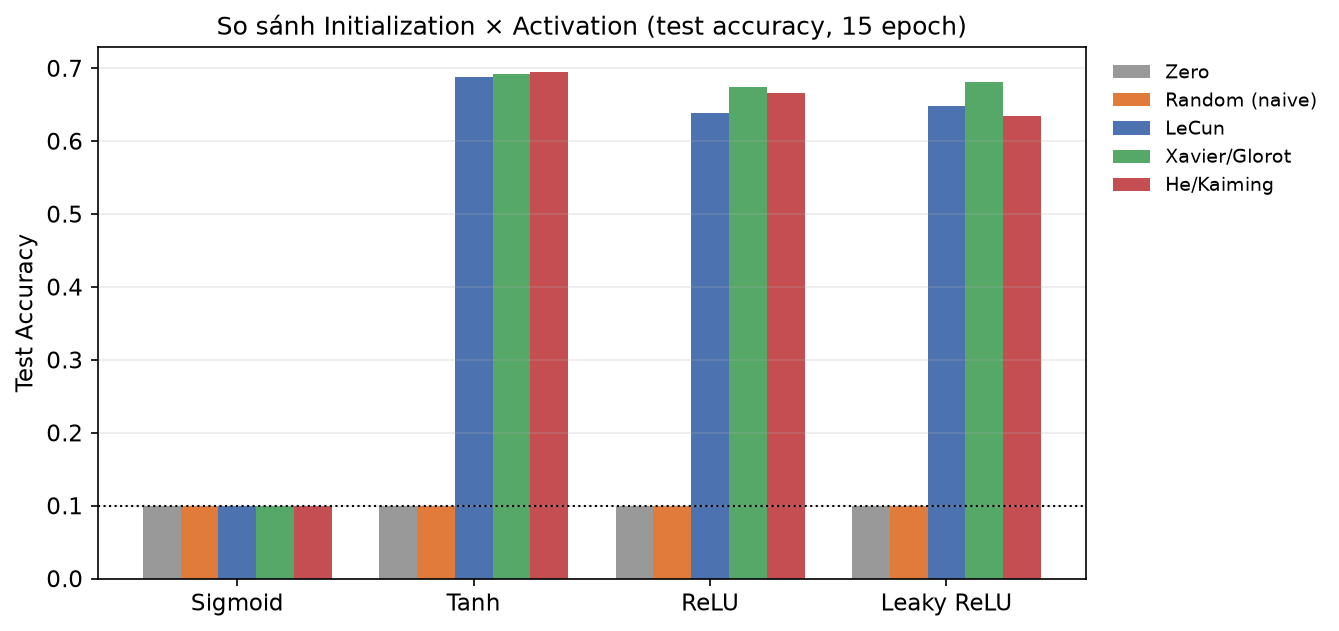
\includegraphics[width=0.82\linewidth]{figures/initialization_comparison.png}
\caption{Test accuracy, toàn bộ lưới $5\times4$ (đường chấm = mức ngẫu nhiên $10\%$).}
\label{fig:initcomp}
\end{figure}

Ba quan sát chính (Hình~\ref{fig:initcomp}, Bảng~\ref{tab:results_grid}):

\begin{enumerate}
\item \textbf{Zero và Random (naive) không bao giờ vượt mức ngẫu nhiên
  ($10\%$)}, với \emph{mọi} activation --- khớp dự đoán lý thuyết
  Mục~\ref{sec:zero} (Zero: gradient lớp ẩn $\equiv0$) và Mục~\ref{sec:random} (Random
  không scale theo $n_{\text{in}}$ nên vẫn vanishing ở độ sâu 6 lớp).
\item \textbf{Sigmoid thất bại với MỌI initialization}, kể cả He/Xavier
  vốn ``đúng lý thuyết'' cho các activation khác. Mục~\ref{sec:discussion}
  phân tích nguyên nhân bằng chính số liệu gradient đo được.
\item \textbf{LeCun/Xavier/He đều hoạt động tốt với Tanh/ReLU/Leaky ReLU}
  ($64$--$69\%$), chênh lệch giữa 3 scheme này nhỏ hơn nhiều so với chênh
  lệch Zero/Random vs.\ có-scale --- khớp việc cả ba đều bảo toàn variance
  tín hiệu đúng bậc-độ-lớn, chỉ khác hệ số nhân ($1$ so với $2$).
\end{enumerate}

\subsubsection*{Đọc chi tiết theo từng activation (cột của Bảng~\ref{tab:results_grid})}

\textbf{Cột Sigmoid.} Cả 5 scheme đều dừng ở $10.0\%$ --- không có ``người
thắng''. Đây không phải lỗi thực nghiệm (đã kiểm tra: mọi cấu hình sigmoid
đều hội tụ về đúng cùng một điểm bias-only, xem thảo luận cơ chế chính
xác ở Mục~\ref{sec:discussion}). Điểm đáng chú ý: \emph{ngay cả về mặt
số học}, 5 giá trị test accuracy của cột này giống nhau tới 3 chữ số thập
phân dù xuất phát từ 5 initialization khác hẳn nhau --- gợi ý mạng học
được đúng \emph{một} hàm hằng số (dự đoán theo tần suất lớp), không phân
biệt được input, bất kể initialization.

\textbf{Cột Tanh.} Kết quả tốt nhất trong toàn lưới (He: $69.4\%$,
Xavier: $69.2\%$, LeCun: $68.9\%$) --- khớp lý thuyết: Tanh có đạo hàm
cực đại $=1$ tại $z=0$ (so với $0.25$ của Sigmoid), ít suy giảm tín hiệu
nhất trong 4 activation được thử, nên ``tha thứ'' cho sai lệch nhỏ giữa 3
scheme LeCun/Xavier/He hơn.

\textbf{Cột ReLU.} Xavier dẫn đầu nhẹ ($67.4\%$) trước He ($66.7\%$)
và LeCun ($63.8\%$) --- như đã thảo luận (Mục~\ref{sec:discussion}),
chênh lệch Xavier/He nằm trong biên độ nhiễu 1-seed, không nên diễn giải
quá mức. LeCun rõ ràng thấp hơn hẳn 2 scheme kia --- hợp lý vì LeCun
không có hệ số bù $\times2$ cho việc ReLU triệt tiêu nửa variance
(Mục~\ref{sec:schemes}).

\textbf{Cột Leaky ReLU.} Xavier tốt nhất ($68.2\%$), He giảm xuống
$63.4\%$ (thấp hơn cả ReLU thường) --- điểm bất ngờ nhẹ, vì Leaky ReLU
có $\mathrm{Var}(a)$ nhỉnh hơn ReLU (phần $z<0$ không hoàn toàn về $0$,
xem Mục~\ref{sec:vanishing}), nên hệ số bù $\times2$ của He có thể hơi
\emph{``quá tay''} cho Leaky ReLU cụ thể ở kiến trúc/learning-rate này ---
một giả thuyết hợp lý nhưng cần thêm thực nghiệm nhiều seed để xác nhận
chắc chắn (không kiểm chứng thêm trong phạm vi báo cáo,
Mục~\ref{sec:limitations}).

\subsection{Gradient norm theo layer (Experiment 7)}

\begin{figure}[H]
\centering
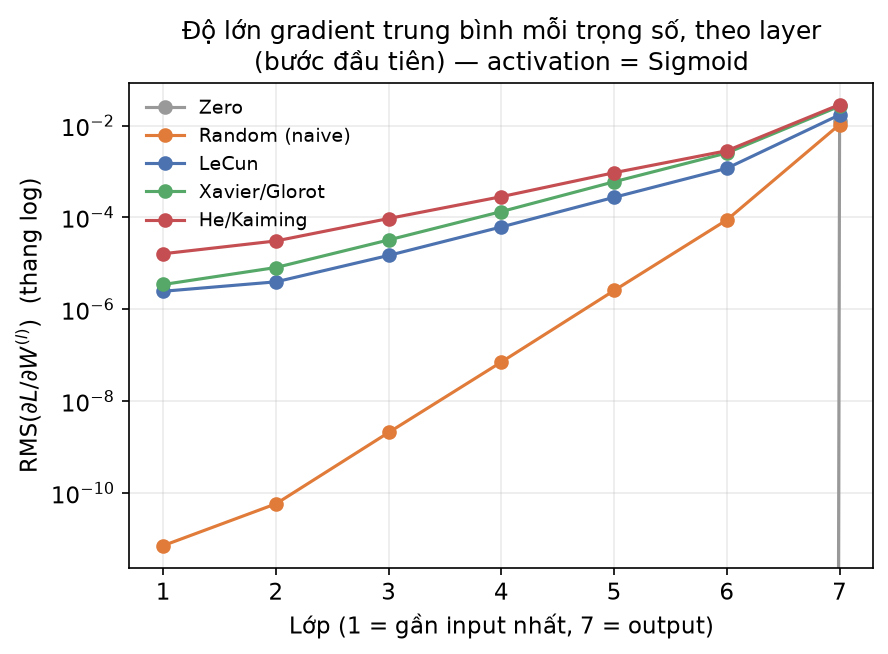
\includegraphics[width=0.72\linewidth]{figures/gradient_norm.png}
\caption{RMS gradient mỗi trọng số theo layer, bước đầu tiên, activation
Sigmoid (thang log). Đường ``Zero'' không hiện được vì gradient đúng bằng
$0$ tại 6 lớp ẩn (Mục~\ref{sec:zero}) --- log của $0$ không xác định.}
\label{fig:gradnorm}
\end{figure}

Hình~\ref{fig:gradnorm} là bằng chứng thực nghiệm rõ nhất cho
Mục~\ref{sec:vanishing}: \textbf{Random (naive)} suy giảm gần \textbf{9 bậc
độ lớn} từ lớp 7 (output) về lớp 1 (gần input), từ $\approx10^{-2}$ xuống
$\approx3\times10^{-11}$ --- vanishing gradient kinh điển do $\sigma=0.01$
không được scale theo $n_{\text{in}}=128$. \textbf{LeCun/Xavier/He} suy
giảm nhẹ hơn nhiều (khoảng 2--3 bậc độ lớn) nhưng \emph{vẫn suy giảm} vì
bản thân $\sigma'(z)\le0.25$ (Sigmoid) co tín hiệu lại ở mỗi lớp bất kể
weight scale đã đúng.

\subsection{Activation variance theo layer}

\begin{figure}[H]
\centering
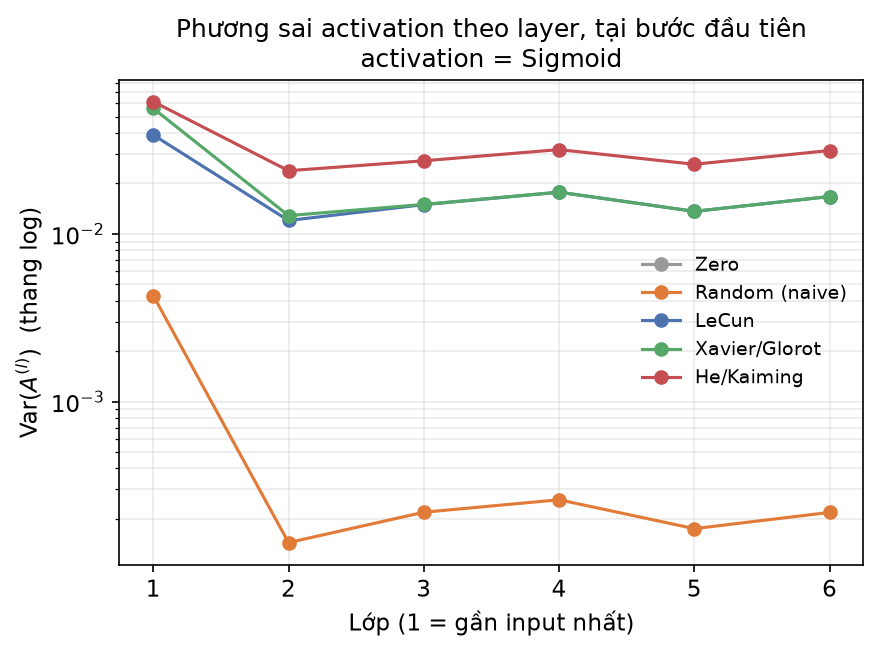
\includegraphics[width=0.72\linewidth]{figures/activation_variance.png}
\caption{Phương sai activation theo layer, bước đầu tiên, activation Sigmoid (thang log).}
\label{fig:actvar}
\end{figure}

Variance activation của Random (naive) ổn định ở mức rất thấp
($\approx2$--$3\times10^{-4}$) ngay từ lớp 2 trở đi --- các neuron gần như
bão hoà quanh $\sigma(0)=0.5$ với biến thiên cực nhỏ, giải thích trực
tiếp vì sao gradient (Hình~\ref{fig:gradnorm}) cũng vanish nặng: activation
gần như hằng số $\Rightarrow$ không mang thông tin phân biệt các mẫu.
LeCun/Xavier/He giữ variance cao hơn hẳn ($10^{-2}$), ổn định qua các lớp.

\subsection{Weight variance theo layer}

\begin{figure}[H]
\centering
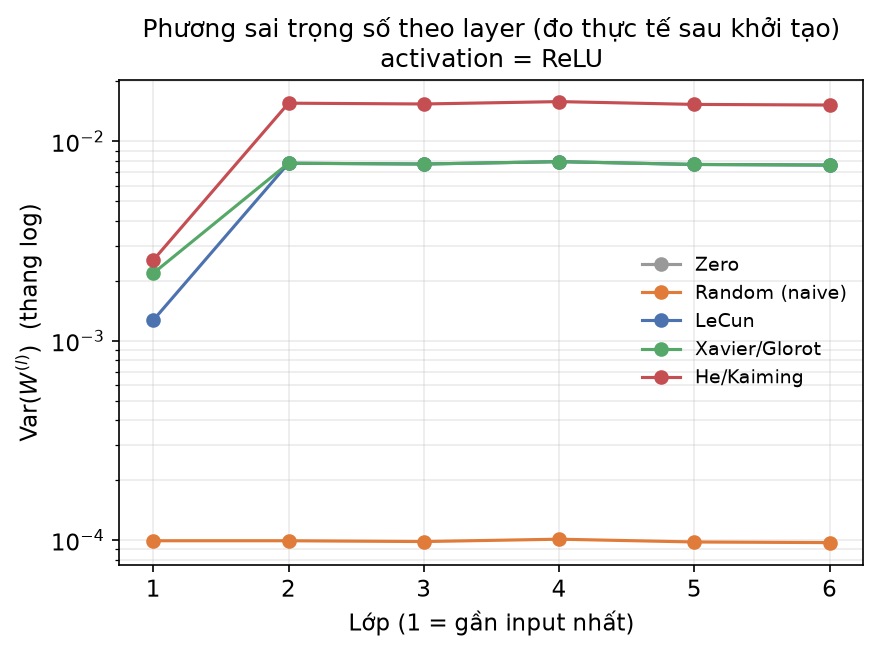
\includegraphics[width=0.72\linewidth]{figures/weight_variance.png}
\caption{Phương sai trọng số theo layer (đo thực tế ngay sau khởi tạo, activation ReLU).}
\label{fig:wvar}
\end{figure}

Hình~\ref{fig:wvar} xác nhận việc lấy mẫu $W\sim\mathcal N(0,\mathrm{Var}(W))$
trong \texttt{src/initialization.py} đúng như công thức Bảng~\ref{tab:schemes}:
variance đo được của He luôn cao hơn Xavier, cao hơn LeCun, ở \emph{mọi}
lớp (thứ tự $2/n_{\text{in}} > 2/(n_{\text{in}}+n_{\text{out}}) > 1/n_{\text{in}}$
khi $n_{\text{in}}=n_{\text{out}}$ --- đúng cho 5/6 lớp ẩn có cùng kích
thước $128\times128$).

\subsection{Loss và Accuracy theo epoch (Experiment 8)}

\begin{figure}[H]
\centering
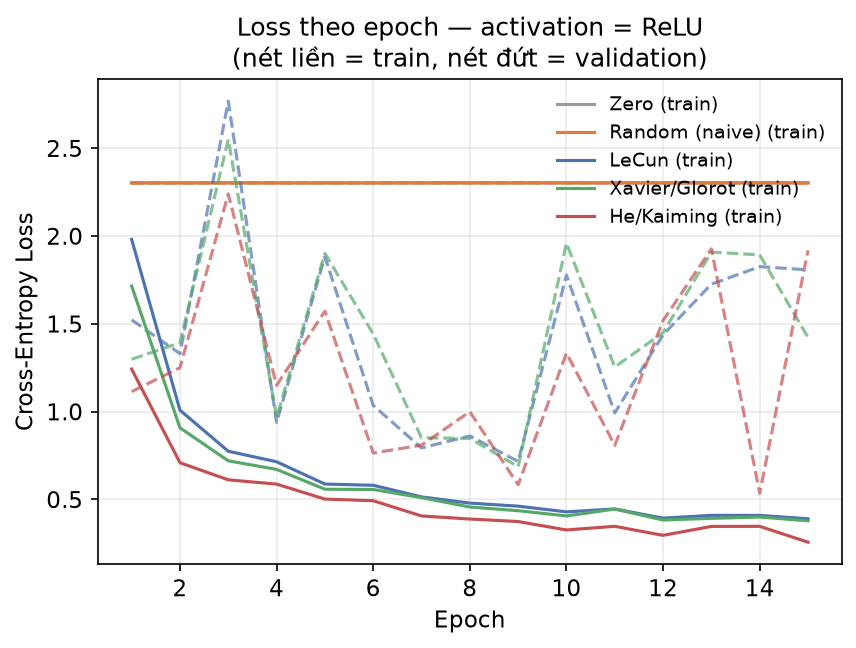
\includegraphics[width=0.72\linewidth]{figures/loss_comparison.png}
\hfill
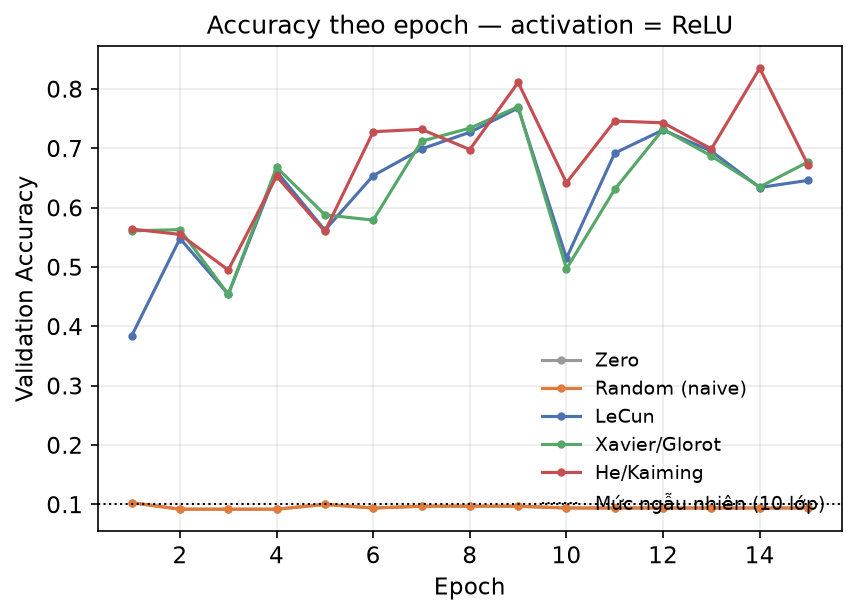
\includegraphics[width=0.72\linewidth]{figures/accuracy_comparison.png}
\caption{Loss (trái) và validation accuracy (phải) theo epoch, activation
ReLU. Zero/Random nằm sát mức ngẫu nhiên (đường chấm) suốt 15 epoch.}
\label{fig:convergence}
\end{figure}

LeCun/Xavier/He hội tụ nhanh (accuracy $>60\%$ ngay từ epoch 4--5) nhưng
validation loss/accuracy dao động khá mạnh giữa các epoch --- tập
validation chỉ $1\,000$ mẫu (nhiễu thống kê đáng kể) cộng với không có
learning-rate decay/momentum để làm mượt quỹ đạo hội tụ (thảo luận thêm ở
Mục~\ref{sec:limitations}).

\subsection{Phân phối gradient và activation (histogram)}

\begin{figure}[H]
\centering
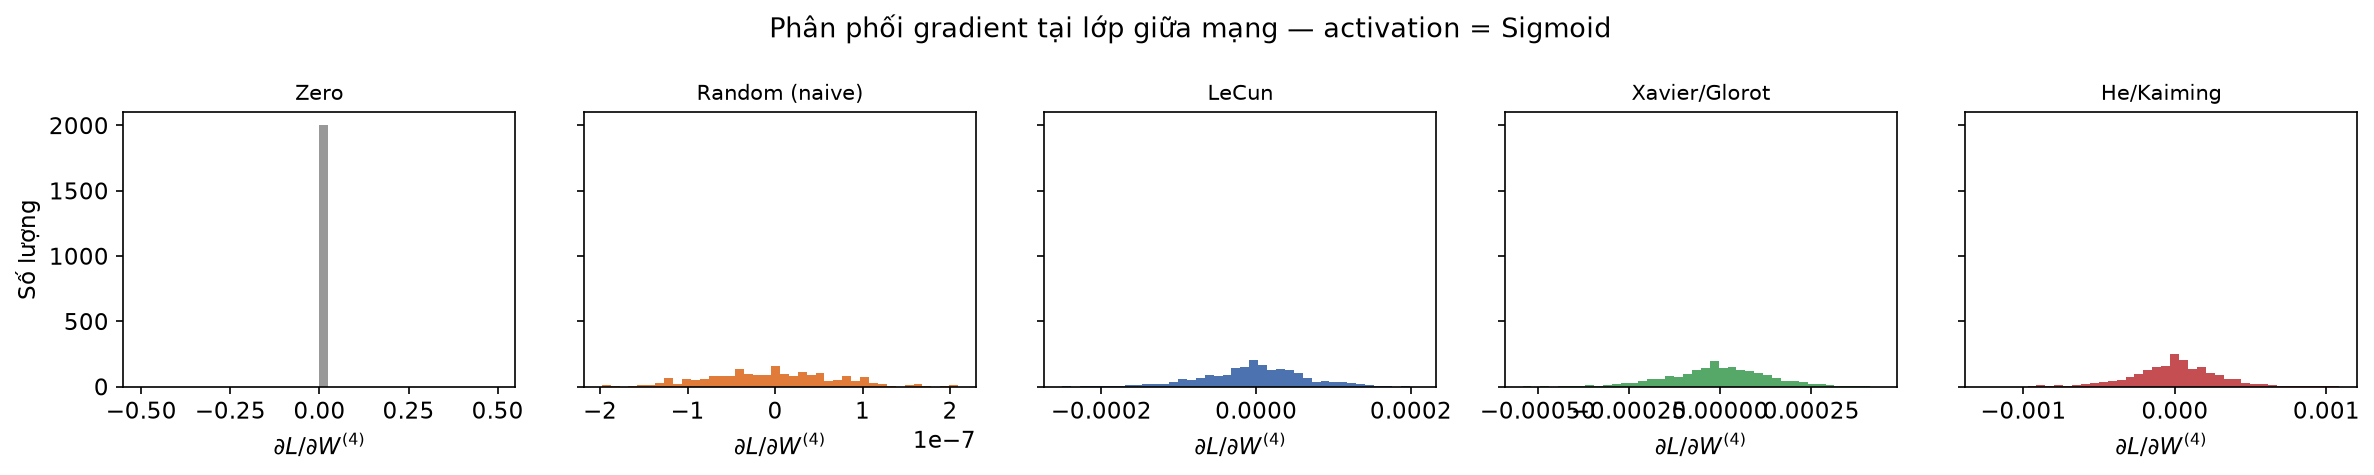
\includegraphics[width=\linewidth]{figures/gradient_histogram.png}
\caption{Phân phối gradient tại lớp giữa mạng (lớp 3), activation Sigmoid, 5 scheme.}
\label{fig:gradhist}
\end{figure}

\begin{figure}[H]
\centering
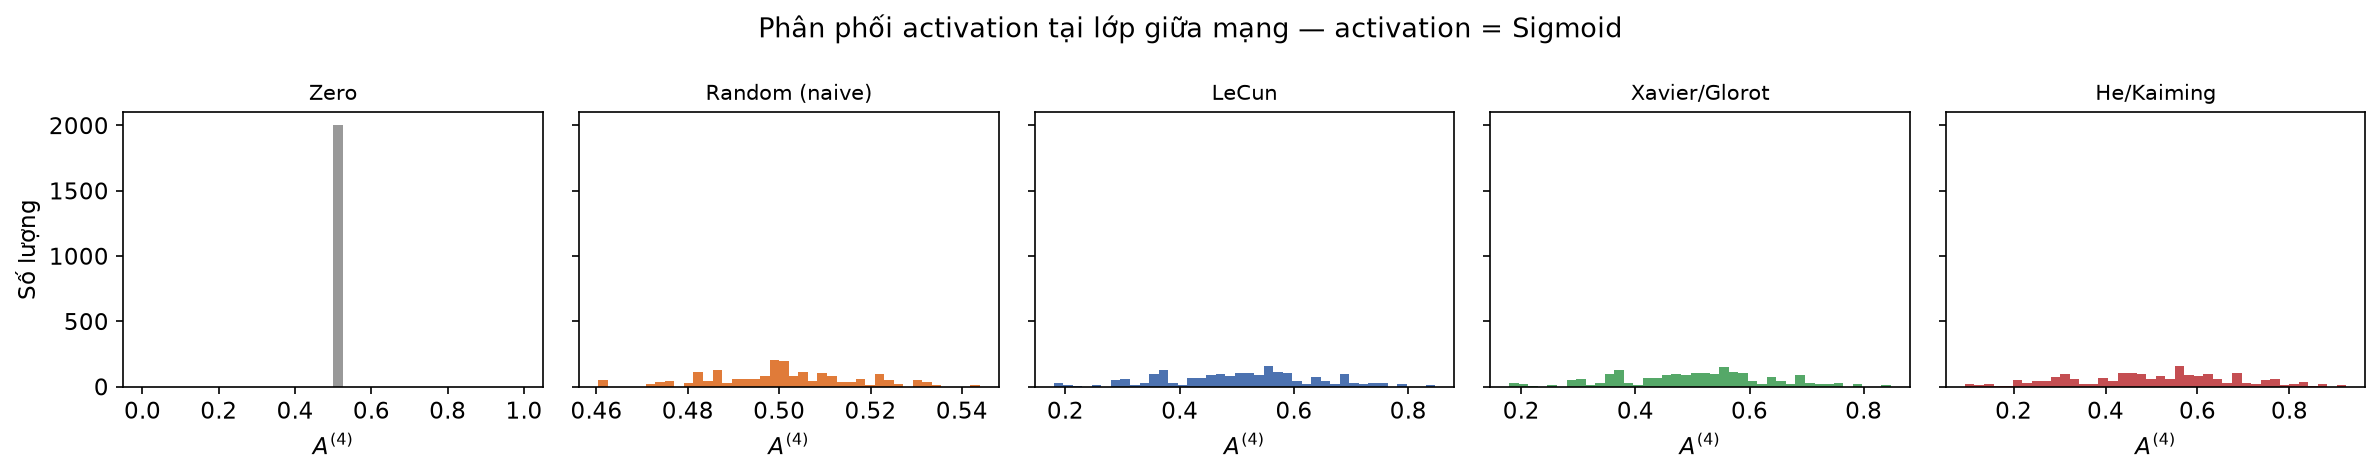
\includegraphics[width=\linewidth]{figures/activation_histogram.png}
\caption{Phân phối activation tại lớp giữa mạng (lớp 3), activation Sigmoid, 5 scheme.}
\label{fig:acthist}
\end{figure}

Histogram gradient (Hình~\ref{fig:gradhist}) của Random (naive) co cụm sát
$0$ với biên độ nhỏ hơn nhiều bậc so với LeCun/Xavier/He --- cùng một hiện
tượng vanishing nhìn từ góc phân phối thay vì trung bình/norm. Histogram
activation (Hình~\ref{fig:acthist}) của Zero co cụm hoàn toàn tại $0.5$
(hằng số, đúng như phân tích Mục~\ref{sec:zero}: $a=\sigma(0)=0.5$ với
mọi mẫu vì $z\equiv0$).

\subsection{Toàn cảnh: loss theo epoch của cả 20 cấu hình}
\label{sec:smallmult}

Các Hình~\ref{fig:convergence}--\ref{fig:acthist} chỉ trích một lát cắt
(1 activation) để dễ đọc. Hình~\ref{fig:smallmult} trình bày \textbf{toàn
bộ lưới $5\times4=20$} cùng lúc, mỗi ô một cấu hình --- để người đọc tự
kiểm chứng không có cấu hình nào bị ``chọn đẹp'' (\en{cherry-picking}) khi
báo cáo chỉ trưng lát cắt ReLU/Sigmoid ở các mục trước.

\begin{figure}[H]
\centering
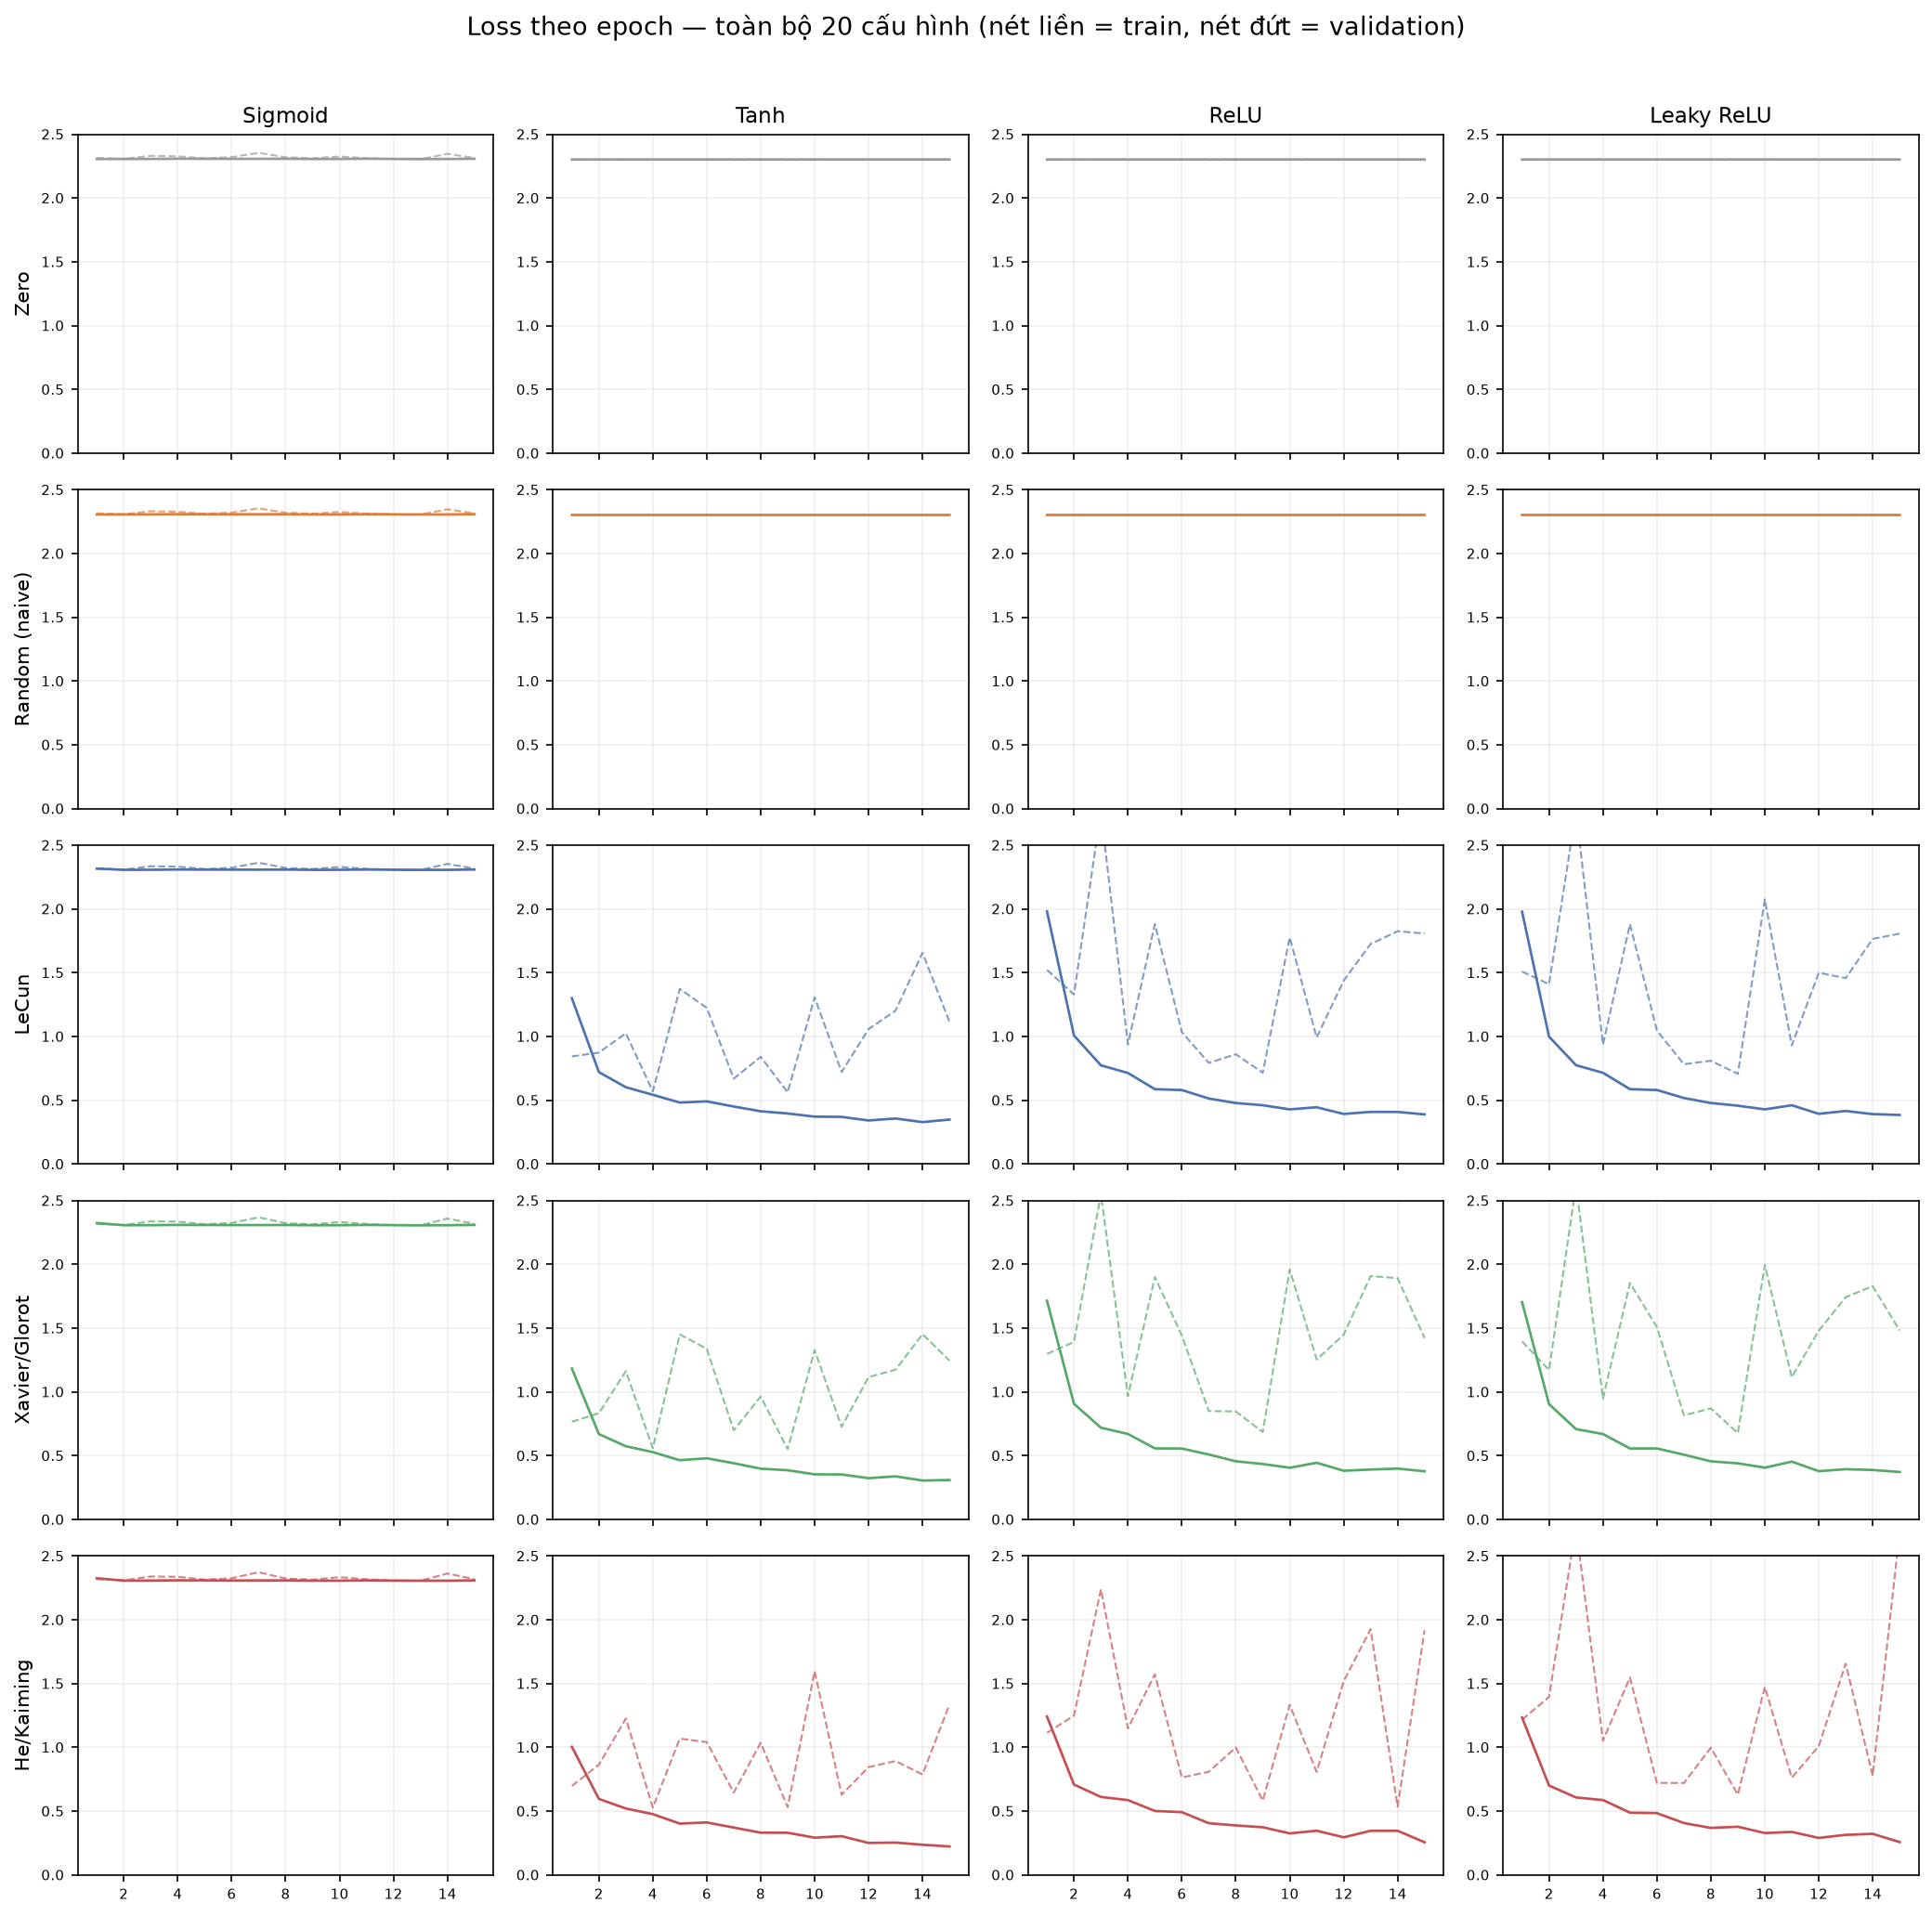
\includegraphics[width=0.92\linewidth]{figures/small_multiples_loss.png}
\caption{Loss theo epoch, toàn bộ 20 cấu hình (hàng = scheme, cột =
activation; nét liền = train, nét đứt = validation; trục tung cắt ở
$2.5$ để các đường hội tụ không bị nén). Hai hàng Zero/Random phẳng
tuyệt đối ở mọi cột --- xác nhận trực quan Bảng~\ref{tab:results_grid}
không có ngoại lệ ẩn nào ngoài lát cắt đã trình bày.}
\label{fig:smallmult}
\end{figure}

Quan sát thêm không thấy rõ ở các lát cắt trước: với cột \textbf{ReLU} và
\textbf{Leaky ReLU}, validation loss của LeCun/Xavier/He đều dao động
mạnh và có xu hướng \textbf{tăng nhẹ trở lại} sau epoch $\approx10$ trong
khi train loss tiếp tục giảm đều --- dấu hiệu \emph{overfitting nhẹ}
(model bắt đầu khớp quá sát $5\,000$ mẫu train, không cải thiện thêm trên
val) ở nửa sau quá trình huấn luyện. Đây là hành vi bình thường của một
MLP không regularization trên tập train nhỏ, không phải triệu chứng của
vanishing/exploding gradient --- một điểm dễ nhầm nếu chỉ nhìn một
lát cắt đơn lẻ.

%==============================================================================
% 10. DISCUSSION
%==============================================================================
\section{Thảo luận}
\label{sec:discussion}

\subsection{Vì sao Sigmoid thất bại ngay cả với He/Xavier?}

Đây là kết quả
đáng chú ý nhất của thực nghiệm (Bảng~\ref{tab:results_grid}): lý thuyết
Mục~\ref{sec:schemes} nói He/Xavier ``bảo toàn variance tín hiệu'', nhưng
điều đó chỉ đúng về \emph{weight scale} --- nó không thể bù cho việc
$\sigma'(z)\le0.25$ \textbf{luôn luôn đúng}, bất kể variance của $z$ là
bao nhiêu. Với 6 lớp, hệ số suy giảm trần do riêng activation gây ra đã là
$0.25^6\approx2.4\times10^{-4}$ --- cộng thêm $15$ epoch với SGD thuần
($\eta=0.05$, không momentum) là không đủ để vượt qua mức suy giảm này
trong thời gian huấn luyện ngắn của báo cáo. Số liệu Mục~\ref{sec:results}
xác nhận đúng cơ chế này: gradient RMS lớp 1 của Sigmoid+He chỉ
$\approx1.6\times10^{-5}$ (so với $\approx2.8\times10^{-2}$ của
ReLU+He) --- khác $0$ (không ``chết'' như Zero-init) nhưng quá nhỏ để tạo ra
bước cập nhật đáng kể ở LR đang dùng.

\textbf{Nguyên nhân thứ hai, độc lập với trần đạo hàm: lệch tâm của
Sigmoid gây dao động dích dắc (zig-zagging).} $\sigma'(z)\le0.25$ giải
thích tín hiệu \emph{yếu}; nhưng ngay cả khi tín hiệu đủ mạnh, Sigmoid còn
một vấn đề thứ hai làm SGD hội tụ chậm: $\sigma(z)\in(0,1)$
\textbf{không đối xứng quanh $0$} ($\mathbb E[\sigma(z)]\approx0.5>0$,
cùng bản chất lệch tâm dương đã phân tích cho ReLU ở Mục~\ref{sec:schemes},
chỉ khác Sigmoid lệch tâm nhiều hơn hẳn vì miền giá trị bị nén hoàn toàn
vào $(0,1)$). Theo công thức Mục~\ref{sec:matrixform},
$\partial L/\partial W^{(l)}=(A^{(l-1)})\T\delta^{(l)}$, tức với \emph{một}
neuron output cố định $j$, dấu của $\partial L/\partial w_{ij}$ với mọi
$i$ chỉ phụ thuộc dấu của $\delta_j$ --- vì $A^{(l-1)}_{i}>0$ với
\textbf{mọi} $i$ (Sigmoid luôn dương). Hệ quả: \textbf{mọi trọng số đi vào
cùng một neuron buộc phải tăng đồng loạt hoặc giảm đồng loạt ở mỗi bước
cập nhật} --- không thể di chuyển tự do theo từng hướng riêng như khi input
đã căn giữa quanh $0$. Về mặt hình học, quỹ đạo Gradient Descent trong
không gian trọng số bị ép đi theo đường \textbf{dích dắc}
(\en{zig-zagging}) thay vì đường thẳng ngắn nhất tới cực tiểu --- đúng
hiện tượng mà \citet{lecun1998efficient} khuyến nghị tránh bằng cách
\emph{căn giữa input} (\en{centering}) trước khi đưa vào mạng; ở đây vấn
đề tái xuất hiện ngay giữa các lớp ẩn vì Sigmoid tự làm mất tính căn giữa
mà chính lớp trước đã có. Cơ chế này giải thích thêm phần nào vì sao
Sigmoid+He/Xavier hội tụ chậm \emph{ngay cả khi} gradient chưa suy giảm
tới mức triệt tiêu hoàn toàn.

\textbf{Bài học}: initialization tốt là \emph{điều kiện cần}, không phải
\emph{điều kiện đủ}, để tránh vanishing gradient. Với activation bão hoà
(Sigmoid) ở mạng đủ sâu, cần thêm các biện pháp khác (nhiều epoch hơn,
learning rate cao hơn, Batch Normalization, hoặc đơn giản là đổi sang
ReLU/Tanh) --- đây chính là lý do lịch sử Deep Learning dần bỏ Sigmoid làm
activation ẩn cho mạng sâu, dù Sigmoid vẫn còn hữu ích ở lớp output cho
bài toán phân loại nhị phân.

\subsection{Đối chiếu dự đoán lý thuyết với số liệu}

\textbf{So với lý thuyết ở Mục~\ref{sec:schemes}--\ref{sec:vanishing}}: dự
đoán ``Zero/Random thất bại, LeCun/Xavier/He thành công với Tanh/ReLU'' khớp
hoàn toàn với thực nghiệm, ở cả lưới chính (Mục~\ref{sec:results}) lẫn
thực nghiệm độ sâu bổ sung (Mục~\ref{sec:depthexp}). Dự đoán ``He tốt hơn
Xavier cho ReLU'' \textbf{không nên được diễn giải là đã xác nhận} ở quy
mô thực nghiệm này: He đạt $66.7\%$, Xavier đạt $67.4\%$ trên
\textbf{đúng một seed} ($seed{=}42$) --- Xavier nhỉnh hơn về mặt số học,
nhưng chênh lệch $0.7$ điểm phần trăm này hoàn toàn nằm trong biên độ
dao động ngẫu nhiên bình thường giữa các lần chạy (minibatch shuffling,
thứ tự cập nhật) của \emph{cùng một} scheme, không có ý nghĩa thống kê
(\en{statistically insignificant}) khi chỉ có $n{=}1$ quan sát mỗi
scheme. \textbf{Không nên dùng con số này làm căn cứ kết luận Xavier vượt
trội hơn He cho ReLU} --- kết luận đúng đắn duy nhất rút ra được là ``cả
hai đều hoạt động tốt, ở cùng một bậc hiệu năng'', không phải một thứ tự
xếp hạng dứt khoát giữa hai scheme (muốn xếp hạng đáng tin cậy cần lặp
lại nhiều seed và kiểm định thống kê, xem Mục~\ref{sec:limitations}).

Kết quả thực nghiệm độ sâu (Mục~\ref{sec:depthexp}) bổ sung một phát hiện
\emph{ngoài dự đoán của riêng lý thuyết variance}: tại $L{=}12$, He vẫn
giữ gradient khởi tạo ổn định (đúng dự đoán Mục~\ref{sec:schemes}) nhưng
test accuracy sụp xuống $32.6\%$ --- tuy nhiên (xem phân tích chi tiết
ở Mục~\ref{sec:depthexp}) đây là \textbf{suy sụp năng lực khái quát hoá
do overfitting} (train loss thấp, test loss vọt lên $5.409$), \textbf{không
phải} một dạng vanishing/exploding gradient chưa được mô hình hoá. Điều
này khẳng định rõ ranh giới của Mục~\ref{sec:init}: phân tích variance
tĩnh mô tả đúng \emph{bước khởi tạo}, nhưng không --- và không có ý định
--- mô tả toàn bộ động lực hội tụ và khái quát hoá của quá trình huấn
luyện nhiều epoch sau đó; đây là hai lớp vấn đề tách biệt cần hai lớp
công cụ tách biệt (initialization cho lớp đầu, regularization/early
stopping/thêm dữ liệu cho lớp sau).

\subsection{Liên hệ tới kiến trúc hiện đại}

Bảng khuyến nghị Mục~\ref{sec:schemes} (Bảng~\ref{tab:compat}) vẫn là
điểm khởi đầu hợp lý khi thiết kế mạng mới, nhưng kết quả
Mục~\ref{sec:results}, \ref{sec:depthexp} nhắc nhở rằng với activation
bão hoà hoặc mạng rất sâu, initialization một mình không đủ. Đây chính là
động lực của ba kỹ thuật phổ biến trong kiến trúc hiện đại, mỗi kỹ thuật
giải quyết một khía cạnh khác của cùng vấn đề ``gradient chảy qua mạng
sâu'':

\begin{itemize}
\item \textbf{Batch/Layer Normalization}: chuẩn hoá lại phân phối
  $z^{(l)}$ \emph{sau mỗi lớp}, không chỉ dựa vào việc chọn đúng
  $\mathrm{Var}(W)$ một lần lúc khởi tạo --- giảm mạnh độ nhạy với cả
  initialization lẫn learning rate trong suốt quá trình huấn luyện, không
  chỉ tại bước đầu.
\item \textbf{Residual connection} (ResNet và hầu hết kiến trúc sâu hiện
  đại, gồm cả Transformer): thêm đường tắt $a^{(l)}=a^{(l-1)}+F(a^{(l-1)})$
  --- khi lan truyền ngược, $\partial a^{(l)}/\partial a^{(l-1)} = I + \partial F/\partial a^{(l-1)}$
  luôn có thành phần $I$ (ma trận đơn vị) cộng thêm, nên gradient có một
  ``đường đi tắt'' không bị nhân suy giảm qua $F$, giảm hẳn vấn đề vanishing
  theo cấp số nhân của Mục~\ref{sec:vanishing} kể cả khi mạng có hàng trăm
  lớp.
\item \textbf{Kiến trúc decoder-only/Transformer hiện đại}: thường dùng
  Pre-Layer-Norm (chuẩn hoá \emph{trước} mỗi khối, không phải sau) kết
  hợp He/Xavier-như initialization đã điều chỉnh theo độ sâu (vd.\ scale
  theo $1/\sqrt{2L}$ với $L$ là số lớp) --- một sự tổng hợp trực tiếp của
  cả ba ý tưởng: initialization đúng, chuẩn hoá liên tục, và đường tắt
  gradient.
\item \textbf{Activation tự chuẩn hoá} (ELU~\citep{clevert2016elu},
  SELU~\citep{klambauer2017selu}, xem hộp Mục~\ref{sec:schemes}): tấn
  công trực tiếp vấn đề \emph{lệch tâm dương} của ReLU thay vì dùng thêm
  một lớp chuẩn hoá riêng --- đổi activation để bản thân phép forward đã
  tự giữ $\mathbb E[a]\approx0$, $\mathrm{Var}(a)\approx1$ qua mỗi lớp mà
  không cần tham số học thêm như BatchNorm.
\end{itemize}

Bốn kỹ thuật trên nằm ngoài phạm vi thực nghiệm của báo cáo (kiến trúc cố
định là MLP thuần, không residual/normalization/activation tự chuẩn hoá
--- Mục~\ref{sec:methodology}); động lực lý thuyết cho Residual
connection/BatchNorm vẫn đứng vững độc lập với thực nghiệm của báo cáo
này, dựa trên chính phân tích vanishing/exploding theo cấp số nhân ở
Mục~\ref{sec:vanishing}. Cần nói rõ một điểm dễ hiểu nhầm: điểm gãy tại
$L{=}12$ trong thực nghiệm độ sâu (Mục~\ref{sec:depthexp}) --- theo phân
tích chi tiết ở đó --- là \textbf{suy sụp khái quát hoá do overfitting},
\emph{không phải} vanishing gradient, nên \textbf{không} nên trích dẫn
trực tiếp quan sát $L{=}12$ này làm bằng chứng thực nghiệm cho việc cần
Residual/BatchNorm (hai kỹ thuật đó giải quyết đúng vấn đề gradient, chứ
không trực tiếp giải quyết overfitting). Quan sát $L{=}12$ thay vào đó
minh hoạ một điểm bổ sung, tách biệt: mạng càng sâu (càng nhiều tham số)
thì càng dễ overfit trên tập dữ liệu nhỏ --- một lý do \emph{khác}, độc
lập với vanishing gradient, khiến các kiến trúc sâu hiện đại luôn đi kèm
kỹ thuật regularization (Dropout, weight decay, data augmentation) bên
cạnh Residual/BatchNorm, không thay thế cho nhau.

\subsection{Câu hỏi thường gặp}

\textbf{``Nếu dùng Adam thay vì SGD thì kết quả Sigmoid có khá hơn
không?''} Có thể một phần --- Adam (Mục~\ref{sec:optimizers}) tự động
tăng bước cập nhật cho tham số có gradient lịch sử nhỏ, nên có thể bù một
phần cho gradient nhỏ (nhưng khác $0$) của Sigmoid+He. Tuy nhiên với
Zero-init, gradient đúng bằng $0$ nên Adam cũng không giúp được gì (đã
giải thích ở hộp trực giác Mục~\ref{sec:optimizers}). Báo cáo không kiểm
chứng thực nghiệm giả thuyết này (cố định SGD thuần để giữ fair
experiment, Mục~\ref{sec:limitations}).

\textbf{``Kết quả có đổi nhiều không nếu dùng activation khác cho lớp
output?''} Không --- lớp output trong mọi thực nghiệm của báo cáo luôn là
linear (logits thô), như mô tả ở Mục~\ref{sec:forward},
\ref{sec:methodology}. Đây là lựa chọn chuẩn cho bài toán phân loại nhiều
lớp dùng \texttt{CrossEntropyLoss} (hàm loss tự áp dụng softmax bên
trong), không liên quan tới initialization của các lớp ẩn đang khảo sát.

\textbf{``Tại sao không thử nhiều seed để có khoảng tin cậy?''} Đây chính
là hạn chế lớn nhất đã nêu ở Mục~\ref{sec:limitations} --- một seed duy
nhất mỗi cấu hình là đủ để minh hoạ \emph{xu hướng} (chênh lệch lớn giữa
Zero/Random và LeCun/Xavier/He rõ ràng vượt xa nhiễu ngẫu nhiên), nhưng
không đủ để so sánh \emph{định lượng chính xác} giữa các scheme gần nhau
(vd.\ He vs.\ Xavier cho ReLU).

%==============================================================================
% 11. LIMITATIONS
%==============================================================================
\section{Hạn chế}
\label{sec:limitations}

Các hạn chế dưới đây phần lớn là \textbf{lựa chọn có chủ đích} để giữ thực
nghiệm gọn, chạy nhanh trên CPU và giữ đúng nguyên tắc fair experiment
(Mục~\ref{sec:methodology}), không phải sai sót. Mục đích liệt kê rõ ràng
ở đây là để người đọc biết chính xác \emph{phạm vi} mà các kết luận của
báo cáo (Mục~\ref{sec:results}--\ref{sec:discussion}) có thể áp dụng, và
phạm vi nào cần thêm thực nghiệm mới có thể khẳng định.

\begin{itemize}
\item \textbf{Quy mô nhỏ}: subset $5\,000$/$1\,000$/$2\,000$ mẫu, 15
  epoch, để chạy nhanh trên CPU --- không phản ánh kết quả ở quy mô full
  Fashion-MNIST hay nhiều epoch hơn (đặc biệt với Sigmoid, có thể cần rất
  nhiều epoch hơn để vượt qua giai đoạn gradient nhỏ ban đầu).
\item \textbf{Một seed duy nhất} mỗi cấu hình --- không đo được
  variance giữa nhiều lần chạy độc lập, nên các chênh lệch nhỏ (vd. He vs.\
  Xavier trên ReLU, Mục~\ref{sec:discussion}) không thể khẳng định có ý
  nghĩa thống kê.
\item \textbf{SGD thuần, không tinh chỉnh LR riêng} cho từng cấu hình
  (cố ý, để giữ fair experiment) --- nghĩa là một số cấu hình (vd.\
  Sigmoid) có thể học nhanh hơn nếu được tinh chỉnh LR riêng; kết luận
  ``Sigmoid thất bại'' cần hiểu trong đúng phạm vi thiết lập này.
\item \textbf{Không BatchNorm/Dropout/LR schedule} --- cố ý loại bỏ để
  initialization là biến duy nhất, nhưng vì vậy kết quả không đại diện cho
  thiết lập huấn luyện hiện đại (nơi BatchNorm thường giảm đáng kể độ nhạy
  với initialization).
\item \textbf{Validation dao động mạnh} (Hình~\ref{fig:convergence}) do
  tập val nhỏ ($1\,000$ mẫu) --- nên đọc xu hướng chung thay vì giá trị
  từng epoch riêng lẻ.
\item \textbf{Lớp output cũng khởi tạo theo cùng scheme} với các lớp ẩn
  (xem \url{src/models.py}) dù lớp output không có activation phi tuyến
  phía sau --- lựa chọn đơn giản hoá, có thể không tối ưu tuyệt đối nhưng
  không ảnh hưởng tới các kết luận định tính của báo cáo.
\item \textbf{Thực nghiệm độ sâu} (Mục~\ref{sec:depthexp}) dùng $8$ epoch
  (ít hơn $15$ epoch của lưới chính) và cũng chỉ $1$ seed --- hiện tượng
  suy sụp khái quát hoá tại $L{=}12$ của He (Hình~\ref{fig:depthexp}) là
  một quan sát thật nhưng \emph{đơn lẻ}; chưa đủ để khẳng định đây là quy
  luật chung (vd.\ "He luôn overfit tại $L\ge12$") hay đặc thù của đúng
  seed/kiến trúc này. Cần chạy nhiều seed ở các độ sâu lân cận
  ($L{=}11,13$) để xác nhận trước khi coi đây là kết luận tổng quát.
\end{itemize}

Tổng hợp lại: giới hạn lớn nhất xuyên suốt là \textbf{thiếu lặp lại nhiều
seed} --- mọi so sánh \emph{định tính} của báo cáo (Zero/Random thất bại
tuyệt đối, Sigmoid thất bại với mọi scheme, LeCun/Xavier/He thành công rõ
rệt với Tanh/ReLU) đều đủ chắc chắn vì chênh lệch rất lớn so với nhiễu
ngẫu nhiên hợp lý của một seed; nhưng mọi so sánh \emph{định lượng chính
xác} giữa các cấu hình gần nhau (He vs.\ Xavier, điểm gãy độ sâu chính
xác của He) cần thêm thực nghiệm nhiều seed mới nên trích dẫn như số liệu
dứt khoát.

%==============================================================================
% 12. CONCLUSION
%==============================================================================
\section{Kết luận}

Báo cáo trình bày Backpropagation như hệ quả trực tiếp của Chain Rule áp
dụng có hệ thống trên một computational graph (Mục~\ref{sec:chainrule}--\ref{sec:backprop}),
phân biệt rõ với Gradient Descent (Mục~\ref{sec:bp_vs_gd}): Backprop
\emph{tính} gradient, Gradient Descent \emph{dùng} gradient đó để cập nhật
tham số. Về Initialization, báo cáo chứng minh bằng cả suy luận toán học
(Mục~\ref{sec:init}) lẫn thực nghiệm thật (Mục~\ref{sec:results}) rằng lựa
chọn $\theta_0$ ảnh hưởng quyết định tới việc mạng có học được hay không:
Zero-init xoá hoàn toàn khả năng phá vỡ đối xứng (gradient lớp ẩn $\equiv0$,
đo được chính xác bằng $0.0$ trong thực nghiệm); Random (naive) và ngay
cả He/Xavier với activation bão hoà sâu (Sigmoid, 6 lớp) vẫn có thể
vanishing đủ mạnh để chặn đứng việc học trong thời gian huấn luyện ngắn.
Hai chủ đề tưởng như tách biệt của báo cáo hoá ra là hai mặt của cùng một
câu hỏi: \emph{làm sao gradient ``chảy'' xuyên suốt một mạng nhiều lớp mà
không biến mất hay bùng nổ} --- Backpropagation là cơ chế \emph{tính}
dòng chảy đó, Initialization là điều kiện \emph{ban đầu} quyết định dòng
chảy đó có sống sót qua nhiều lớp hay không.

\textbf{Đóng góp cụ thể của báo cáo} (tổng hợp lại các mục thực nghiệm):
(1) triển khai và kiểm chứng Backpropagation thủ công bằng NumPy, khớp
tuyệt đối PyTorch autograd và finite-difference tới sai số $10^{-9}$
(Mục~\ref{sec:gradcheck}); (2) lưới thực nghiệm đầy đủ $5\times4=20$ cấu
hình initialization$\times$activation trên Fashion-MNIST, xác nhận trực
tiếp các dự đoán lý thuyết bằng số liệu đo được, không suy diễn
(Mục~\ref{sec:results}); (3) thực nghiệm bổ sung về độ sâu mạng
(Mục~\ref{sec:depthexp}), cho thấy cả hiện tượng vanishing kinh điển
(Random, suy giảm 12 bậc độ lớn qua 12 lớp) lẫn một giới hạn ít được nhắc
tới của chính He initialization ở độ sâu rất lớn.

\textbf{Hướng mở rộng} nếu có thêm thời gian/tài nguyên (liệt kê đầy đủ ở
Mục~\ref{sec:limitations}): lặp lại lưới thực nghiệm với nhiều seed để có
khoảng tin cậy; thêm Batch Normalization như một biến thực nghiệm thứ ba
để đo trực tiếp mức độ nó làm giảm độ nhạy với initialization (dự đoán ở
Mục~\ref{sec:discussion} nhưng chưa kiểm chứng thực nghiệm); mở rộng thực
nghiệm độ sâu (Mục~\ref{sec:depthexp}) sang kiến trúc có residual
connection để so sánh trực tiếp với MLP thuần.

%==============================================================================
% 13. TAI LIEU THAM KHAO
%==============================================================================
\phantomsection
\addcontentsline{toc}{section}{Tài liệu tham khảo}
{\small \bibliography{references}}

\appendix

%==============================================================================
% PHU LUC A: CODE LISTINGS
%==============================================================================
\section{Mã nguồn Manual Backpropagation}
\label{app:code}

Hai đoạn code cốt lõi của Part A (Mục~\ref{sec:implementation}), trích
nguyên văn từ \url{src/manual_nn.py} và \url{src/initialization.py} ---
toàn bộ báo cáo, notebook và slide đều gọi trực tiếp các hàm này, không
có bản sao chỉnh sửa riêng cho việc trình bày.

\begin{lstlisting}[caption={Forward pass -- src/manual\_nn.py}]
def forward(self, X: np.ndarray) -> np.ndarray:
    """X: (N, n0). Tra ve Yhat: (N, nL). Lop cuoi (output) LUON linear
    (khong qua self.f) -- khop quy uoc dung trong models.py va Phase 2."""
    A = X
    Zs, As = [], [A]
    for l in range(self.n_layers):
        Z = A @ self.W[l] + self.b[l]
        is_last = l == self.n_layers - 1
        A = Z if is_last else self.f(Z)
        Zs.append(Z)
        As.append(A)
    self._cache = {"Zs": Zs, "As": As}
    return A
\end{lstlisting}

\begin{lstlisting}[caption={Backward pass -- src/manual\_nn.py (nguyên văn công thức Mục~\ref{sec:matrixform})}]
def backward(self, Yhat: np.ndarray, Y: np.ndarray) -> dict:
    """Tinh dL/dW[l], dL/db[l] cho moi lop bang chain rule:
        dZ^(l) = dA^(l) o f'(Z^(l))          (o = Hadamard)
        dW^(l) = (A^(l-1))^T dZ^(l)
        db^(l) = 1^T dZ^(l)                   (tong theo truc batch)
        dA^(l-1) = dZ^(l) (W^(l))^T
    Loss: MSE trung binh batch -> dL/dYhat = (Yhat - Y) / N.
    """
    Zs, As = self._cache["Zs"], self._cache["As"]
    N = Y.shape[0]
    grads_W = [None] * self.n_layers
    grads_b = [None] * self.n_layers

    dA = (Yhat - Y) / N  # dL/dA^(L), L = output layer (linear)
    for l in reversed(range(self.n_layers)):
        is_last = l == self.n_layers - 1
        dZ = dA if is_last else dA * self.f_grad(Zs[l])
        A_prev = As[l]  # As[l] = A^(l-1) vi As[0]=X
        grads_W[l] = A_prev.T @ dZ
        grads_b[l] = dZ.sum(axis=0)
        dA = dZ @ self.W[l].T  # dL/dA^(l-1), dung cho vong lap ke tiep
    return {"dW": grads_W, "db": grads_b}
\end{lstlisting}

\begin{lstlisting}[caption={Cong thuc Var(W) cho tung scheme -- src/initialization.py (nguyên văn Bảng~\ref{tab:schemes})}]
def weight_variance(scheme, fan_in, fan_out):
    if scheme == "zero":
        return 0.0
    if scheme == "random_normal":
        return 0.01 ** 2       # sigma co dinh, KHONG scale theo fan_in
    if scheme == "lecun":
        return 1.0 / fan_in
    if scheme == "xavier":
        return 2.0 / (fan_in + fan_out)
    if scheme == "he":
        return 2.0 / fan_in
    raise KeyError(f"Khong biet scheme '{scheme}'")
\end{lstlisting}

%==============================================================================
% PHU LUC B: BANG KET QUA DAY DU
%==============================================================================
\section{Bảng kết quả đầy đủ (20 cấu hình)}
\label{app:fulltable}

Bảng~\ref{tab:fulltable} liệt kê đầy đủ 4 metric (không chỉ test accuracy
như Bảng~\ref{tab:results_grid} Mục~\ref{sec:results}) cho toàn bộ $20$
cấu hình, lấy trực tiếp từ \url{results/tables/initialization_comparison.csv}.

\begin{table}[H]
\centering
\caption{Kết quả đầy đủ: train/val/test loss và test accuracy, 20 cấu hình}
\small
\begin{tabular}{@{}llcccc@{}}
\toprule
\textbf{Scheme} & \textbf{Activation} & \textbf{Train loss} & \textbf{Val loss} & \textbf{Test loss} & \textbf{Test acc.} \\
\midrule
Zero & Sigmoid & 2.309 & 2.315 & 2.314 & 0.100 \\
Zero & Tanh & 2.303 & 2.303 & 2.303 & 0.100 \\
Zero & ReLU & 2.303 & 2.303 & 2.303 & 0.100 \\
Zero & Leaky ReLU & 2.303 & 2.303 & 2.303 & 0.100 \\
\addlinespace
Random & Sigmoid & 2.309 & 2.315 & 2.313 & 0.100 \\
Random & Tanh & 2.303 & 2.303 & 2.303 & 0.100 \\
Random & ReLU & 2.303 & 2.303 & 2.303 & 0.100 \\
Random & Leaky ReLU & 2.303 & 2.303 & 2.303 & 0.100 \\
\addlinespace
LeCun & Sigmoid & 2.309 & 2.317 & 2.315 & 0.100 \\
LeCun & Tanh & 0.349 & 1.116 & 1.098 & \textbf{0.689} \\
LeCun & ReLU & 0.390 & 1.808 & 1.742 & 0.638 \\
LeCun & Leaky ReLU & 0.385 & 1.807 & 1.732 & 0.648 \\
\addlinespace
Xavier & Sigmoid & 2.310 & 2.318 & 2.317 & 0.100 \\
Xavier & Tanh & 0.310 & 1.246 & 1.239 & \textbf{0.692} \\
Xavier & ReLU & 0.378 & 1.423 & 1.373 & \textbf{0.674} \\
Xavier & Leaky ReLU & 0.373 & 1.482 & 1.410 & \textbf{0.682} \\
\addlinespace
He & Sigmoid & 2.310 & 2.319 & 2.317 & 0.100 \\
He & Tanh & 0.223 & 1.337 & 1.329 & \textbf{0.694} \\
He & ReLU & 0.256 & 1.919 & 1.822 & 0.667 \\
He & Leaky ReLU & 0.258 & 2.691 & 2.579 & 0.634 \\
\bottomrule
\end{tabular}
\label{tab:fulltable}
\end{table}

\textbf{Đọc bảng}: cột in đậm là giá trị cao nhất theo cột trong nhóm
Tanh/ReLU/Leaky ReLU (Sigmoid không có cột in đậm vì cả 5 scheme đều
$0.100$ --- không có ``người thắng'', xem thảo luận Mục~\ref{sec:discussion}).
Chênh lệch train loss vs.\ val/test loss ở mọi cấu hình học được (vd.\
He+Tanh: $0.223$ so với $1.337$) phản ánh đúng hiện tượng overfitting
nhẹ đã nêu ở Mục~\ref{sec:smallmult} --- dự kiến với $5\,000$ mẫu train,
không regularization, 15 epoch.

%==============================================================================
% PHU LUC C: CAU HOI PHAN BIEN
%==============================================================================
\section{20 câu hỏi phản biện thường gặp}
\label{app:faq}

Tổng hợp ngắn gọn, dùng để chuẩn bị hỏi--đáp khi bảo vệ báo cáo; mỗi câu
trả lời có trích dẫn mục tương ứng để tra cứu chi tiết.

\begin{enumerate}
\item \textbf{Backpropagation là gì?} Thuật toán tính $\nabla_\theta L$
  hiệu quả bằng Chain Rule áp dụng có hệ thống trên computational graph,
  tận dụng giá trị đã lưu từ forward pass (Mục~\ref{sec:backprop}).
\item \textbf{Vì sao cần Chain Rule?} Vì $L$ là hợp của nhiều phép biến
  đổi lồng nhau qua các lớp; Chain Rule là quy tắc toán học duy nhất cho
  phép tính đạo hàm của một hàm hợp mà không cần khai triển tường minh
  toàn bộ biểu thức (Mục~\ref{sec:chainrule}).
\item \textbf{Backpropagation khác Gradient Descent như thế nào?}
  Backprop \emph{tính} gradient; Gradient Descent \emph{dùng} gradient đó
  để cập nhật tham số ($\theta\leftarrow\theta-\eta\nabla_\theta L$) ---
  hai vai trò tách biệt, không thể hoán đổi (Mục~\ref{sec:bp_vs_gd}).
\item \textbf{Tại sao gradient có thể vanish?} Gradient qua $L$ lớp xấp xỉ
  $g^L$ với $g$ = độ lớn trung bình mỗi đạo hàm cục bộ; nếu $g<1$ (activation
  bão hoà và/hoặc weight scale nhỏ), $g^L\to0$ theo hàm mũ khi $L$ tăng
  (Mục~\ref{sec:vanishing}).
\item \textbf{Tại sao gradient có thể explode?} Cùng cơ chế trên nhưng
  $g>1$ (weight scale quá lớn) khiến $g^L\to\infty$ theo hàm mũ
  (Mục~\ref{sec:vanishing}).
\item \textbf{Tại sao initialize toàn bộ weight = 0 không tốt?} Mọi
  neuron trong một lớp nhận cùng input, cùng trọng số $\Rightarrow$ cùng
  gradient $\Rightarrow$ mãi mãi giống hệt nhau (mất symmetry breaking);
  nếu $W{=}0$ ở mọi lớp, gradient lớp ẩn còn bằng \emph{đúng} $0$, đo được
  thực nghiệm (Mục~\ref{sec:zero}).
\item \textbf{Tại sao phải randomize parameter?} Để phá vỡ đối xứng giữa
  các neuron trong cùng lớp --- điều kiện \emph{cần} nhưng chưa \emph{đủ}
  (còn phải scale đúng theo $n_{\text{in}}$, xem câu 8--10) (Mục~\ref{sec:random}).
\item \textbf{Xavier giải quyết vấn đề gì?} Chọn $\mathrm{Var}(W)=2/(n_{\text{in}}+n_{\text{out}})$
  để dung hoà đồng thời điều kiện giữ ổn định variance khi forward
  ($1/n_{\text{in}}$) và khi backward ($1/n_{\text{out}}$), phù hợp
  activation đối xứng (Tanh/Sigmoid) (Mục~\ref{sec:schemes}).
\item \textbf{He initialization khác Xavier thế nào?} He dùng
  $\mathrm{Var}(W)=2/n_{\text{in}}$ --- gấp đôi Xavier (khi
  $n_{\text{in}}{=}n_{\text{out}}$) để bù việc ReLU triệt tiêu khoảng một
  nửa variance tín hiệu (phần $z<0\to0$) (Mục~\ref{sec:schemes}).
\item \textbf{Tại sao ReLU thường đi với He initialization?} Vì He được
  suy ra \emph{trực tiếp} từ đặc tính của ReLU (hệ số bù $\times2$ ở câu
  9); dùng Xavier cho ReLU vẫn hoạt động (Bảng~\ref{tab:results_grid}: Xavier+ReLU
  $67.4\%$) nhưng không xuất phát từ đúng giả định về activation
  (Mục~\ref{sec:schemes}, \ref{sec:discussion}).
\item \textbf{fan\_in và fan\_out là gì?} $\mathrm{fan\_in}=n_{l-1}$ (số
  input của 1 neuron), $\mathrm{fan\_out}=n_l$ (số neuron lớp sau nhận
  input từ neuron này) --- hai đại lượng quyết định
  $\mathrm{Var}(z)=n_{\text{in}}\mathrm{Var}(W)\mathrm{Var}(x)$ (Mục~\ref{sec:schemes}).
\item \textbf{Initialization ảnh hưởng activation variance như thế nào?}
  $\mathrm{Var}(a^{(l)})\approx r^l\mathrm{Var}(x)$ với
  $r=n_{\text{in}}\mathrm{Var}(W)$ (đã hiệu chỉnh activation) --- xem ví
  dụ số Bảng~\ref{tab:varprop} và số liệu đo thật Hình~\ref{fig:actvar}
  (Mục~\ref{sec:varprop}, \ref{sec:results}).
\item \textbf{Initialization ảnh hưởng gradient variance như thế nào?}
  Cùng cơ chế nhân dồn theo chiều ngược lại (thay $n_{\text{in}}$ bằng
  $n_{\text{out}}$ trong phân tích) --- đo thực tế ở Hình~\ref{fig:gradnorm}
  (Mục~\ref{sec:vanishing}, \ref{sec:results}).
\item \textbf{Tại sao network càng sâu càng nhạy với initialization?} Vì
  hệ số $r$ (hoặc $g$) bị nhân dồn theo \emph{luỹ thừa của số lớp} --- một
  sai lệch nhỏ ở $r$ so với $1$ bị khuếch đại theo hàm mũ của độ sâu,
  chứng minh trực tiếp bằng thực nghiệm độ sâu (Hình~\ref{fig:depthexp},
  Mục~\ref{sec:depthexp}).
\item \textbf{PyTorch autograd thực hiện điều gì?} Tự động xây và duyệt
  ngược computational graph để tính gradient --- về bản chất toán học
  cũng là Backpropagation, chỉ tự động hoá việc xây đồ thị thay vì viết
  tay (Mục~\ref{sec:implementation}).
\item \textbf{Manual gradient và autograd khác nhau như thế nào?} Không
  khác về kết quả (Mục~\ref{sec:gradcheck}: sai số $\approx10^{-9}$, chỉ
  là sai số làm tròn) --- chỉ khác về việc \emph{ai} xây computational
  graph và tính đạo hàm cục bộ: người viết code (manual) hay framework
  (autograd).
\item \textbf{Gradient checking dùng để làm gì?} Đối chiếu gradient tính
  bằng backprop với gradient tính bằng finite-difference (chậm nhưng
  đáng tin) để \emph{cô lập lỗi} khi tự viết backward pass thủ công
  (Mục~\ref{sec:gradcheck}).
\item \textbf{Có phải initialization tốt luôn đảm bảo model tốt không?}
  Không --- là điều kiện \emph{cần}, không phải \emph{đủ}, và thất bại có
  thể tới từ những \emph{nguyên nhân hoàn toàn khác nhau}. Thực nghiệm
  Sigmoid (Mục~\ref{sec:discussion}) thất bại vì \emph{vanishing gradient}
  (thiếu tín hiệu học); thực nghiệm độ sâu $L{=}12$
  (Mục~\ref{sec:depthexp}) thất bại vì \emph{overfitting/suy sụp khái
  quát hoá} dù gradient hoàn toàn bình thường --- hai cơ chế thất bại
  khác hẳn nhau nhưng cùng cho kết quả bề mặt là "model tệ", nên chẩn
  đoán đúng nguyên nhân (nhìn cả train loss lẫn test loss, không chỉ
  accuracy) là bước bắt buộc trước khi chọn cách khắc phục.
\item \textbf{Initialization có còn quan trọng khi dùng BatchNorm/LayerNorm
  không?} Có, nhưng \emph{ít nhạy cảm hơn nhiều} --- Batch/Layer Norm
  chuẩn hoá lại phân phối tín hiệu sau \emph{mỗi} lớp trong suốt huấn
  luyện, không chỉ dựa vào việc chọn đúng $\mathrm{Var}(W)$ một lần lúc
  khởi tạo (Mục~\ref{sec:discussion}).
\item \textbf{Initialization và optimizer có quan hệ như thế nào?} Độc
  lập về vai trò (Mục~\ref{sec:bp_vs_gd}) nhưng phối hợp trong thực tế:
  optimizer thích ứng (Adam) có thể bù \emph{một phần} gradient nhỏ do
  initialization dưới mức tối ưu, nhưng không cứu được trường hợp gradient
  bằng đúng $0$ (Zero-init) --- hộp trực giác Mục~\ref{sec:optimizers}.
\end{enumerate}

%==============================================================================
% PHU LUC D: NOTEBOOK
%==============================================================================
\section{Danh mục notebook}
\label{app:notebooks}

Ngoài script trong \texttt{experiments/}, project kèm $5$ Jupyter notebook
(\texttt{notebooks/01}--\texttt{05}, đã chạy sẵn với output thật, không
cần chạy lại để xem kết quả) --- mỗi notebook tương ứng một mục của báo
cáo, dùng khi cần trình bày tương tác thay vì đọc PDF tĩnh:

\begin{table}[H]
\centering
\small
\begin{tabular}{@{}p{2.5cm}p{8.8cm}p{2.4cm}@{}}
\toprule
\textbf{Notebook} & \textbf{Nội dung} & \textbf{Mục liên quan} \\
\midrule
\texttt{01\_\allowbreak derivative\_\allowbreak demo} & Đạo hàm là độ nhạy ($y=x^2$, tiếp tuyến); Chain Rule trên ví dụ $x\to z\to a\to L$ & Mục~\ref{sec:chainrule} \\
\texttt{02\_\allowbreak manual\_\allowbreak backprop} & Chạy \texttt{ManualMLP} trên đúng ví dụ 2 lớp của báo cáo; đối chiếu PyTorch autograd trực tiếp trong notebook & Mục~\ref{sec:scalar} \\
\texttt{03\_\allowbreak gradient\_\allowbreak check} & Chạy lại \texttt{run\_gradient\_check.py}, hiển thị report JSON đầy đủ & Mục~\ref{sec:gradcheck} \\
\texttt{04\_\allowbreak initialization\_\allowbreak experiment} & Nạp lại \texttt{results/} (không chạy lại 20 cấu hình), hiển thị bảng + 4 hình chính & Mục~\ref{sec:results} \\
\texttt{05\_\allowbreak analysis} & Bảng pivot test accuracy đầy đủ + 3 quan sát chính, dùng cùng logic phân tích với Mục~\ref{sec:discussion} & Mục~\ref{sec:discussion} \\
\bottomrule
\end{tabular}
\label{tab:notebooks}
\end{table}

%==============================================================================
% PHU LUC E: BANG THUAT NGU
%==============================================================================
\section{Bảng thuật ngữ Việt--Anh}
\label{app:glossary}

\begin{table}[H]
\centering
\small
\begin{tabular}{@{}p{4.6cm}p{4.6cm}p{4.6cm}@{}}
\toprule
Đạo hàm --- \en{Derivative} & Lan truyền tiến --- \en{Forward Propagation} & Khởi tạo tham số --- \en{Parameter Initialization} \\
Đạo hàm riêng --- \en{Partial Derivative} & Lan truyền ngược --- \en{Backpropagation} & Phá vỡ đối xứng --- \en{Symmetry Breaking} \\
Gradient & Đồ thị tính toán --- \en{Computational Graph} & Gradient biến mất --- \en{Vanishing Gradient} \\
Ma trận Jacobian --- \en{Jacobian} & Hàm kích hoạt --- \en{Activation Function} & Gradient bùng nổ --- \en{Exploding Gradient} \\
Quy tắc chuỗi --- \en{Chain Rule} & Hàm mất mát --- \en{Loss Function} & Chuẩn hoá theo lô --- \en{Batch Normalization} \\
Trọng số dùng chung --- \en{Weight Sharing} & Nhân từng phần tử --- \en{Hadamard Product} & Kết nối tắt --- \en{Residual/Skip Connection} \\
Lô (dữ liệu) --- \en{Batch} & Suy giảm trọng số --- \en{Weight Decay} & Học sâu --- \en{Deep Learning} \\
Siêu tham số --- \en{Hyperparameter} & Quá khớp --- \en{Overfitting} & Kiểm tra gradient --- \en{Gradient Checking} \\
\bottomrule
\end{tabular}
\caption{Đối chiếu thuật ngữ tiếng Việt -- tiếng Anh dùng trong báo cáo}
\label{tab:glossary}
\end{table}

\end{document}
